\documentclass[11pt,a4paper]{report}

\usepackage{changepage}
\usepackage{microtype}

\usepackage{xcolor}
\definecolor{sapienzaRed}{HTML}{802433}

% Italian language settings
\usepackage[utf8]{inputenc}
\usepackage[T1]{fontenc}
\usepackage[italian,english]{babel}

% Set the font to Times New Roman (or a similar serif font)
\usepackage{mathptmx}

% Set the page margins to 2.5 cm on all sides
\usepackage[a4paper, top=2.8cm, bottom=2.8cm, left=3.2cm, right=2.8cm]{geometry}

% Load packages for pseudocode
\usepackage{algorithm}
\usepackage{algpseudocode}

% Set line spacing to 1.5
\usepackage{setspace}
\onehalfspacing

% Load packages for mathematical symbols and environments
\usepackage{amsmath}
\usepackage{amsfonts}
\usepackage{amssymb}

% Load package for small captions in figures and tables
\usepackage[font=small]{caption}

% Invisible boundary for figures and tables to prevent them from floating too far from their reference point
\usepackage{placeins}

% Load package for including graphics such as images and figures
\usepackage{graphicx}

% Load package for adjusting the width of text blocks
\usepackage{fancyhdr}


% Used in tables
\usepackage{booktabs}
\usepackage{multirow}

% used for tree
\usepackage{tikz}
\usetikzlibrary{positioning}

% Redefine the chapter title format and spacing
\usepackage{titlesec}
\titleformat{\chapter}[display]
  {\normalfont\huge\bfseries}{\chaptertitlename\ \thechapter}{15pt}{\Huge}
\titlespacing*{\chapter}{0pt}{10pt}{25pt}

% Load package for creating colored boxes and listings
\usepackage[most]{tcolorbox}
\usepackage{listings}

% Define custom colors for code to use for code snippets
\definecolor{codebg}{RGB}{250,250,252}
\definecolor{codeframe}{RGB}{218,224,233}
\definecolor{codetitlebg}{RGB}{238,242,246}
\definecolor{codetitle}{RGB}{33,37,41}
\definecolor{codeblue}{RGB}{0,80,180}
\definecolor{codegreen}{RGB}{34,139,34}
\definecolor{codegray}{RGB}{120,120,120}

% C code listing environment with custom styling
\newtcblisting[auto counter, number within=chapter]{clisting}[2][]{
    enhanced,
    listing only,
    arc=2mm,
    boxrule=0.7pt,
    top=0.8pt,                 
    bottom=0.8pt,              
    colback=codebg,
    colframe=codeframe,
    title=\textbf{Listing \thetcbcounter:} #2,
    coltitle=codetitle,
    attach boxed title to top left={xshift=10pt, yshift=-\tcboxedtitleheight/2},
    boxed title style={
        colback=codetitlebg,
        colframe=codeframe,
        boxrule=0.7pt,
        arc=1.5mm
    },
    listing options={
        language=C,
        basicstyle=\ttfamily\footnotesize,
        keywordstyle=\color{codeblue}\bfseries,
        commentstyle=\color{codegreen}\itshape,
        numbers=left,
        numberstyle=\tiny\color{codegray},
        stepnumber=1,
        numbersep=8pt,
        showstringspaces=false,
        tabsize=4,
        breaklines=true,
        columns=flexible
    },
    #1
}

% Terminal-like code listing environment with custom styling
\newtcblisting{lightterminal}[1][]{
    listing only,
    arc=1.5mm,
    boxrule=0.6pt,
    top=3pt,
    bottom=3pt,
    left=6pt,
    right=6pt,
    colback=codebg,
    colframe=codeframe,
    listing options={
        basicstyle=\ttfamily\scriptsize\color{black},
        breaklines=true,
        columns=fullflexible,
        keepspaces=true,
        numbers=none
    },
    #1
}

% Configuration for the page header in a chapter page
\pagestyle{fancy}
\fancyhf{}                              % Clear all header and footer fields
\fancyhead[L]{\nouppercase{\leftmark}} % Chapter title in the header on the left
\fancyhead[R]{\textbf{\thepage}}        % Page number in the header on the right
\renewcommand{\headrulewidth}{0.4pt}    % Set the thickness of the horizontal line in the header

% Configuration for the page header in a plain page (e.g., chapter start)
\fancypagestyle{plain}{
    \fancyhf{}                          % Clear all header and footer fields
    \fancyhead[R]{\textbf{\thepage}}    % Only the page number in the header on the right
    \renewcommand{\headrulewidth}{0pt}  % No horizontal line in the header
}

% Enable numbers for subsubsection and let them show in the contents table
\setcounter{secnumdepth}{3}
\setcounter{tocdepth}{3}

% Bibliography management with biblatex
\usepackage[backend=biber,style=numeric,sorting=none]{biblatex}
\usepackage{xurl} % Allows line breaks in URLs in the bibliography
\addbibresource{references.bib}

% Allows links in the contents
\usepackage{hyperref}
% Allows links for the bibliography
\hypersetup{
    colorlinks=true,       
    linkcolor=black,       
    citecolor=blue!70!black, 
    urlcolor=blue!80!black   
}

% ----------------------------------------------------------------------------------------
\begin{document}

% Title page configuration
\begin{titlepage}
    \sffamily

    % No page number on the title page
    \thispagestyle{empty}

    % Logo of Sapienza aligned to the left
    \begin{flushleft}
        
\includegraphics[width=6cm]{images/sapienza_logo.png}
    \end{flushleft}

    \vspace{2cm}

    % Content of the title page with adjusted width and no automatic indentation
    \begin{adjustwidth}{1.5cm}{0cm}

        % Set the paragraph indentation to zero for the title page content
        \setlength{\parindent}{0pt}

        % Thesis title
        {\LARGE \color{sapienzaRed}
        Secure Satellite Communication: \\
        Performance and cryptographic analysis of \\
        chaotic injected AES resistant to side-channel attacks \\ 
        targeting the S-box via machine unlearning
        \par}

        \vspace{3.7cm}

        % Faculty and degree information
        {\small \color{sapienzaRed}
        Faculty of Information Engineering, Computer Science and Statistics \\
        Bachelor's Degree in Computer Science
        \par}

        \vspace{1.5cm}

        % My name and ID number
        {\normalsize
        \textbf{Simone Descontus} \\
        ID number 2116496 \\[0.3cm]
        
\includegraphics[height=1.2cm]{images/mySignature.png}
        \par}

        \vspace{1cm}

        % Advisor information
        {\normalsize
        Advisor \\
        Prof. Emiliano Casalicchio \\[0.3cm]
%        \includegraphics[height=1.2cm]{images/profSignature.png}
        \par}

        \vfill
        Academic Year 2025/2026

    \end{adjustwidth}
\end{titlepage}

% New page for the copyright and contact information
{\newpage

% Set the paragraph indentation to zero for the title page content
\setlength{\parindent}{0pt}

% No page number on this page
\thispagestyle{empty} 

% Add vertical space to center the content vertically on the page
\vspace*{\fill}

% Add a horizontal line across the width of the page
\rule{\textwidth}{0.4pt}

\vspace{0.3cm}

{\textbf{Secure Satellite Communication: Performance and cryptographic analysis of chaotic injected AES resistant to side-channel attacks targeting the S-box via machine unlearning.}} \\
Sapienza University of Rome

\vspace{0.4cm}

\copyright\ 2026 Simone Descontus. All rights reserved.

\vspace{0.4cm}

This thesis has been typeset by \LaTeX.

\vspace{0.4cm}

Author's email: \texttt{simo.desk04@gmail.com}

\vspace{1cm} % Margine finale rispetto al bordo inferiore della pagina
}

\cleardoublepage
\thispagestyle{empty}

\vspace*{0.28\textheight}
\begin{flushright}
    \begin{minipage}{0.70\textwidth}
        \raggedleft
        \textit{It's time for something new, now.}\\
    \end{minipage}
\end{flushright}
\cleardoublepage


% Contents page
\pagenumbering{roman}

\cleardoublepage
\thispagestyle{myheadings}
\markright{}
\vspace*{1.2cm}
{\noindent\Large\bfseries Abstract\par}
\vspace{0.4cm}
\addcontentsline{toc}{chapter}{Abstract}

Satellite Communications (SATCOM) represent a critical backbone of modern global infrastructure, making the confidentiality and integrity of transmitted data paramount. 
To comply with the stringent SWaP (Size, Weight, and Power) constraints of space-grade hardware, aerospace standards designate AES-256-GCM as the default authenticated encryption protocol. 
In embedded deployments, the algorithm typically relies on pre-computed Look-Up Tables (LUTs) for the S-Box substitution to reduce execution time and energy consumption. 
However, static LUT accesses introduce deterministic physical leakages, exposing the cipher to Side-Channel Attacks (SCAs) that can be drastically accelerated through Machine Learning (ML).

Building upon the chaotic injection framework proposed by Kumar et al., this thesis presents a proof-of-concept C implementation that extends the open-source \texttt{tiny-aes-c} library with the GCM mode of operation and integrates nine distinct chaotic maps (1D, 2D, and 3D). 
To ensure architectural viability for SATCOM, this work introduces a scalar chaotic state optimization and a \texttt{once-per-block} update strategy. 
Empirical evaluations confirm that the modified cipher preserves its cryptographic randomness (passing the NIST SP 800-22 suite) 
while reducing the temporal and energetic overhead with the \texttt{once-per-block} approach to negligible levels ($\approx 0.5\%$--$4\%$, with at most 56 extra bytes of memory). 
Furthermore, a simulated ML-assisted SCA (combining a Random Forest classifier with an algebraic Divide-and-Conquer strategy) achieves a $100\%$ key recovery rate on standard AES-256-GCM, 
while failing completely against the chaotic variants.

Being purely software-defined, the proposed countermeasure can be deployed via Over-the-Air (OTA) updates to both legacy spacecraft already in orbit and constrained terrestrial terminals, 
providing robust side-channel resilience without requiring hardware modifications.


\newpage
\tableofcontents 

\cleardoublepage
\pagenumbering{arabic}

\chapter{Introduction}
With the rapid expansion and increasing accessibility of satellite technologies, ensuring the confidentiality and integrity of data transmitted via Satellite Communications (SATCOM) has become more critical than ever. 
Official aerospace standards designate \textit{AES-256-GCM}~\cite{AES256-GCM} as the default cryptographic protocol for space communications, owing to the low encryption latency of symmetric-key cryptography 
and the robust integrity guarantees provided by the Galois/Counter Mode (GCM) authentication tag.

However, spacecraft must operate under strict \texttt{SWaP} (Size, Weight, and Power) constraints imposed by the harsh space environment. 
To comply with these limitations, the vast majority of embedded satellite implementations rely on pre-computed Look-Up Tables (LUTs) during the \textsc{SubBytes()} routine, 
avoiding the computationally expensive dynamic calculation of multiplicative inverses over $\mathrm{GF}(2^{8})$ that would otherwise increase both execution time and energy consumption. 
While LUTs yield a substantial performance boost, they introduce a severe micro-architectural vulnerability: 
memory accesses to static tables inevitably generate physical power leakages proportional to the processed byte values. 
Adversaries can capture these leakages and leverage advanced Machine Learning (ML) models to render complex Side-Channel Attacks (SCAs) practically feasible.

Conventional countermeasures typically rely on dedicated hardware cryptographic extensions (such as AES-NI) to bypass memory-based LUTs altogether. 
However, such hardware solutions not only increase power consumption and manufacturing costs, but are also completely inapplicable to legacy satellites already deployed in orbit.

\section{Thesis Objective}
Inspired by the foundational work of Kumar et al.~\cite{KumarPaper}, the primary objective of this thesis is to develop a proof-of-concept implementation of \textit{AES with chaotic injection}. 
This is achieved by extending the open-source \texttt{tiny-aes-c} library~\cite{tinyAES} and adapting it to comply with modern satellite communication standards through the integration of the \textit{AES-256-GCM} mode of operation~\cite{AES256-GCM}.

Furthermore, this study aims to analyze the integration of various chaotic maps within the cipher's architecture. 
These configurations are rigorously benchmarked to evaluate execution time, memory footprint, and energy consumption, 
thereby identifying the optimal solution for the resource-constrained SATCOM environment. 
Concurrently, statistical and cryptographic tests verify that altering the standard encryption algorithm does not degrade its fundamental cryptographic properties.

Building upon these analyses, the thesis proposes an architectural optimization tailored for satellite communications. 
A comprehensive comparison is provided between the baseline chaotic algorithm proposed by Kumar et al. and a modified iteration engineered to yield superior performance metrics, 
rendering it highly appropriate for space applications.

Lastly, significantly diverging from the scope of Kumar et al.~\cite{KumarPaper}, this research simulates a Machine Learning-based Side-Channel Attack (SCA) aiming for complete key recovery. 
This simulation serves a critical dual purpose: it demonstrates a devastating threat vector that is entirely feasible against standard AES-256-GCM in current SATCOM architectures, 
while simultaneously proving that the proposed chaotic implementation successfully immunizes the system against such advanced profiling attacks.

To ensure the full reproducibility of this research, the complete C codebase, the statistical and performance benchmarking suites, 
and the Machine Learning side-channel attack scripts are publicly available in a dedicated GitHub repository~\cite{simodesk_aes_chaotic}.

\section{Thesis Structure}
The remainder of this thesis is organized as follows:
\begin{itemize}
    \item \textbf{Chapter 2} provides an in-depth analysis of the state-of-the-art in satellite communications, detailing its architectural segments, 
    the major security threats targeting each segment, and the defensive strategies currently deployed or under investigation.
    
    \item \textbf{Chapter 3} focuses on a rigorous algorithmic analysis of the AES-256-GCM standard, detailing the mathematical mechanics of both the core block cipher routines and the GCM authenticated encryption mode.
    
    \item \textbf{Chapter 4} introduces the chaotic injection framework proposed by Kumar et al.~\cite{KumarPaper}, 
    presents the architectural optimizations designed to minimize overhead on constrained devices, and details the taxonomy of the nine evaluated chaotic systems.
    
    \item \textbf{Chapter 5} presents the empirical tuning methodology used to select the optimal parameters for each chaotic map, 
    validates their randomness properties via the official NIST Statistical Test Suite~\cite{NISTRandomnessTestSuite}, 
    and benchmarks execution time, memory footprint, and energy consumption for both the \texttt{once-per-round} and \texttt{once-per-block} update strategies.
    
    \item \textbf{Chapter 6} details the empirical simulation of a Machine Learning-assisted Side-Channel Attack targeting complete key recovery, 
    illustrating the attack's architecture and demonstrating the resilience of the chaotic-injected S-Box LUT against it.
    
    \item \textbf{Chapter 7} summarizes the main findings of this research and outlines potential directions for future work.
\end{itemize}




% ====================================================================================================

% ====================================================================================================

\chapter[Background and State-of-the-Art of Satellite Communications]{Background and State-of-the-Art of \\ Satellite Communications}
Satellite communications (SATCOM) are vastly different from how they appeared just a few decades ago. 
At that time, space-based communications were mainly represented by government activities, characterized by larger and more expensive satellites than the ones used today. 
This era is also known as the \textit{old space}~\cite[p. 377]{aLotOfReferences}, a term often used to describe the space applications that emerged during the Cold War.

On the other hand, since the beginning of the \textit{new space} era~\cite[p. 377--398]{aLotOfReferences}, 
the steadily decreasing cost of satellite launches and rapid technological progress have populated orbit with commercial satellites serving a wide range of applications. 
Primary examples include \textit{telecommunications and broadband connectivity}, which provide internet access even in remote regions hard to reach with terrestrial infrastructure~\cite[p. 373--381]{aLotOfReferences}, 
as well as \textit{television broadcasting and multimedia streaming}, which leverage wide satellite coverage to meet the constant demand for high-quality content delivery~\cite[p. 373--381]{aLotOfReferences}. 
Furthermore, SATCOM systems are extensively employed for \textit{Earth observation}: thanks to more affordable spacecraft, private entities can now launch dedicated programs for environmental analysis alongside traditional meteorological monitoring~\cite[p. 372--381]{aLotOfReferences}.

In addition, satellite networks enable everyday services such as the \textit{Global Positioning System (GPS)}~\cite[p. 378--381]{aLotOfReferences}, 
which is relied upon daily by individuals and numerous industrial sectors for route planning and resource tracking. 
Similarly, the \textit{Internet of Things (IoT)} heavily depends on SATCOMs: given the heterogeneous nature of IoT devices, ranging from smart homes to transport fleets, 
achieving seamless global coverage is essential and is effectively addressed via space-based links~\cite[p. 372]{aLotOfReferences}. 
Finally, a new frontier is emerging with \textit{Satellite-as-a-Service (SataaS)}. 
Although launch costs have dropped significantly, deploying proprietary spacecraft remains financially prohibitive for many private companies that would otherwise benefit from satellite coverage. 
To address this challenge, major aerospace operators lease onboard resources to third-party users, granting them access to space infrastructure without the need for dedicated launches~\cite{SataaS}.

Along with the opportunities offered by the \textit{new space}, the critical requirements of the \textit{old space} have not diminished. 
Today, satellite communications remain essential for handling mission-critical data exchanges, such as those required by aviation and maritime operations~\cite[p. 397--398]{aLotOfReferences}, 
as well as for the coordination of rescue services in disaster or crisis situations~\cite[p. 388--389]{aLotOfReferences}.

Given the critical nature of the communications handled by SATCOM systems, 
it is becoming increasingly important to protect the information shared within these networks from malicious actors.
To fully understand the scale of these security challenges and how threats can compromise the network,
it is essential to analyze its underlying infrastructure. A modern SATCOM system is not a monolithic entity, but rather a complex, distributed architecture. Breaking down this infrastructure into its fundamental segments is a crucial step to accurately identify the specific attack surfaces that adversaries might exploit.

\section{SATCOM Architecture}
\begin{figure}[htbp]
    \centering
    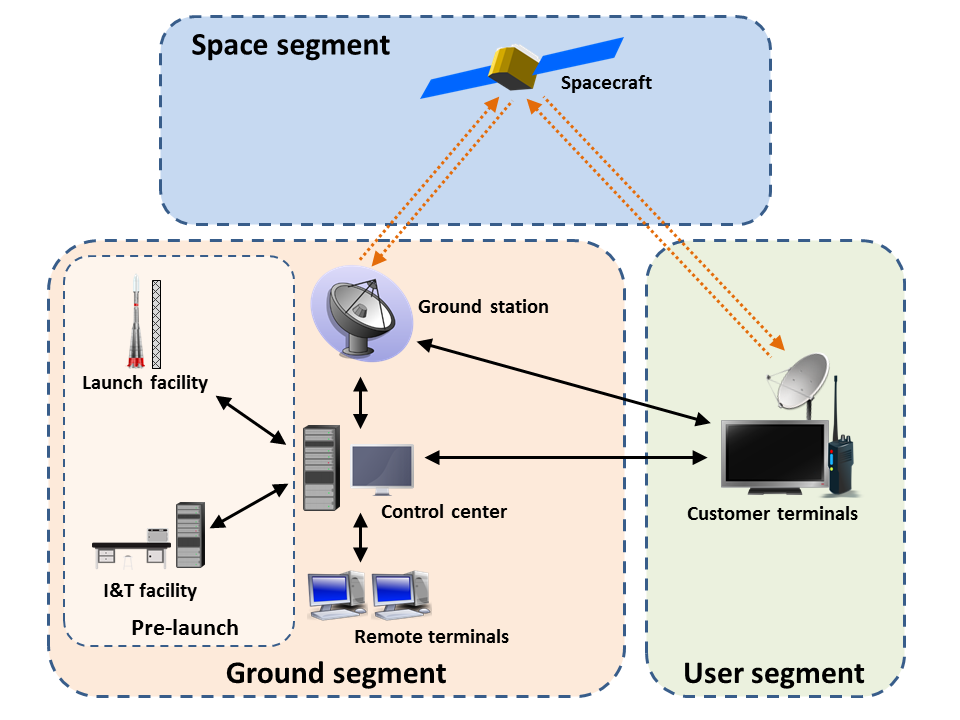
\includegraphics[width=0.6\textwidth]{images/segment.png}
    \caption[Architectural segments of a satellite system]\small{{Architectural overview of space, ground, and user segments in satellite systems~\cite{wiki_ground_segment}.}}
    \label{fig:sat_segments}
\end{figure}

Satellite communications are typically classified into three fundamental segments, although the exact categorization may vary across the literature.
One common classification framework, as described in the extended SATCOM state-of-the-art analysis provided by Salim et al.~\cite{aLotOfReferences}, divides the architecture into the \textit{space segment}, the \textit{ground segment}, and the \textit{link segment}. 
In this model, the \textit{ground Segment} encompasses both the \textit{ground Stations}, which act as gateways for devices lacking direct satellite communication capabilities,
and the \textit{user segment}, which consists of end-user terminals equipped for space links. 
Another classification model still includes the \textit{space segment} and the \textit{ground segment}, 
but explicitly separates the \textit{user segment}, treating the \textit{link segment} merely as a passive communication channel~\cite[p. 5671]{LEO_MEO_GEO}. 

While all these components are crucial to maintain the network's operability, this thesis will adopt the classification proposed in~\cite{aLotOfReferences}, 
grouping the ground stations and end-user devices under a unified \textit{ground segment} is conceptually sound for terrestrial entities. 

\subsection{Space Segment}
The space segment is represented by the satellites in orbit, each composed of the \textit{bus}, which handles onboard systems such as power and thermal management, 
and the \textit{payload}, which is the part of the spacecraft designed to fulfill the satellite's specific mission~\cite[p. 381--383]{aLotOfReferences}. 
Examples of payloads include telescopes to analyze distant objects or sensors to measure spatial properties.

Depending on the satellite's mission, its orbital height from Earth can vary radically~\cite{LEO_MEO_GEO}:
\begin{itemize}
    \item \textit{Low Earth Orbit (LEO)}: due to their low altitude, usually between 500 and 1200 km, 
    these types of satellites are ideal for extending terrestrial networks thanks to their low latency (around 30 ms).
    However, because they are so close to the Earth, it is often necessary to deploy a group of interconnected \textit{LEO} satellites,
    known as a \textit{satellite constellation}, in order to cover a wider area of the planet.
    Additionally, because of the high risk of collision with space debris, the lifetime of \textit{LEO} spacecraft is around 5 to 7 years, 
    which is usually shorter than that of other satellites.

    \item \textit{Medium Earth Orbit (MEO)}: usually positioned at an altitude of 2000 to 20000 km, 
    they represent a midpoint between coverage and latency (around 125 ms). 
    A significant share of \textit{MEO} spacecraft function as GPS satellites, and typically 6 units are necessary in order to provide adequate service. 
    Because of their intermediate position, \textit{MEO} satellites often serve as relay nodes between \textit{LEO} and \textit{GEO} satellites. 
    Finally, their operational lifetime is estimated at 10 to 15 years, depending on their altitude and exposure to radiation.

    \item \textit{Geostationary Equatorial Orbit (GEO)}: operating in the highest orbital layer at approximately 36000 km,
    these spacecraft take exactly 24 hours to complete an orbit, appearing stationary to an observer on Earth. 
    Thanks to their high altitude, they can cover one-third of the entire planet's surface, making them ideal for broadcasting. 
    However, it is important to account for the latency accumulated during transmission (around 600 ms).
    Due to their distance from the planet and the large quantity of resources needed to launch \textit{GEO} spacecraft, they are usually built to last longer, typically around 15 to 20 years.

\end{itemize}

\subsection{Ground Segment}
This segment represents the terrestrial infrastructure that communicates 
with satellites. Depending on the role of the receiver or sender, it can 
be classified into several sub-components, the primary ones being~\cite[p. 383--384]{aLotOfReferences}:
\begin{itemize}
    \item \textit{Ground Stations (GS)}: equipped with dedicated hardware, they can transmit and receive signals even from the most distant satellites. 
    A vast amount of traffic passes through them, as the majority of terrestrial devices lack the necessary peripherals to communicate directly with 
    spacecraft.
    
    \item \textit{Mission Control Centers (MCC)}: their role is to ensure the satellite's mission continues undisturbed by analyzing the telemetry 
    sent by the spacecraft. Telemetry consists of messages transmitted by the satellites containing critical information, such as their exact orbit or 
    internal hardware measurements; this data allows operators to detect anomalies and perform necessary corrective actions. 

    \item \textit{User Segment}: this component comprises all the end-user devices, which receive messages after they are forwarded by the 
    \textit{Ground Stations}. Moreover, devices equipped with the necessary peripherals to communicate directly with the \textit{space segment}, such 
    as ships, airplanes, and Satellite TV, also fall into this category. 
\end{itemize}

\subsection{Link Segment}
This segment is represented by the radio waves that link the Earth to space and the satellites to one another, as well as the hardware 
components used to establish these connections. Specifically, the \textit{link segment} can be categorized as follows~\cite[p. 381]{aLotOfReferences}:
\begin{itemize}
    \item \textit{Ground-to-Ground}: connects the \textit{ground stations} to the \textit{user segment} and vice versa.

    \item \textit{Ground-to-Space}: also known as the \textit{uplink}, it represents the communication path from the \textit{ground segment} 
    to the \textit{space segment}.

    \item \textit{Space-to-Ground}: also known as the \textit{downlink}, it represents the communication path from the \textit{space segment} 
    to the \textit{ground segment}.

    \item \textit{Space-to-Space}: connects the spacecraft within the \textit{space segment} to one another, even across different orbital altitudes.
\end{itemize}

\section{SATCOM Threats}
Due to the distributed architecture of SATCOM networks, security threats targeting any individual segment must be rigorously addressed. 
Tampering with a single component can have cascading effects, jeopardizing the other segments and compromising both the spacecraft's mission and the 
broader network to which it is connected. Some threats associated with each segment are outlined below.

\subsection{Space Segment Threats}
While spacecraft are physically out of reach for potential attackers, this physical isolation does not exempt the \textit{space segment} from cyber threats.

Examples include \textit{software attacks}, in which malicious software could be introduced into the satellite's systems via the \textit{link segment}.
Alternatively, in a \textit{Satellite-as-a-Service (SataaS)} architecture, an attacker could exploit the shared infrastructure by gaining access to the spacecraft's resources under the guise of a legitimate user. 
Furthermore, \textit{Denial of Service (DoS)} attacks pose a significant threat to the \textit{space segment}, as an excessive volume of requests sent to the targeted satellite could overwhelm its processing capabilities, temporarily or permanently disrupting its mission.

Beyond software vulnerabilities, \textit{hardware attacks} target the physical infrastructure of the satellite. 
A particularly insidious example is the \textit{supply chain attack}, which compromises the manufacturing process of the spacecraft by exploiting the decentralized production models typical of the \textit{new space} industry~\cite[p. 386--389]{aLotOfReferences}. 

Although significantly harder to mount and execute, another critical threat to the \textit{space segment} is posed by \textit{kinetic or anti-satellite (ASAT) weapons}. 
These systems consist of high-energy beams or physical interceptors that aim to blind the spacecraft's communications or physically destroy its components~\cite[p. 5677]{LEO_MEO_GEO}.

Finally, another catastrophic threat is the risk of \textit{satellite hijacking}. 
Through command spoofing techniques, an attacker could force the spacecraft to deviate from its intended orbit, often leading to the complete destruction of the satellite as it burns up upon atmospheric reentry~\cite[p. 386--389]{aLotOfReferences}.

\subsection{Ground Segment Threats}
Compared to the \textit{space segment}, the \textit{ground segment} represents a much more accessible entry point for attackers due to its terrestrial location.
Moreover, despite the physical distance between \textit{Ground Stations} and the spacecraft, the impairment of a terrestrial facility can easily jeopardize the satellite itself. 
For instance, malware contaminating a station on Earth could easily be transferred to the \textit{space segment} via the \textit{link segment}.

Similar to the threats facing the space infrastructure, \textit{software attacks} could lead to the temporary deactivation of the communication channels used to send messages to the \textit{space segment}. 
If the compromised facility is a \textit{Mission Control Center (MCC)}, operators would be unable to monitor the satellite's telemetry or detect potential anomalies. 
Consequently, a synchronized cyberattack targeting the \textit{Space Segment} simultaneously would go completely unnoticed.

While \textit{Denial of Service (DoS)} and \textit{Distributed Denial of Service (DDoS)} attacks also pose a significant threat to the \textit{ground segment}, 
a vulnerability exclusively tied to the terrestrial infrastructure is \textit{Unauthorized Access to Ground Stations}. 
If physical or logical authentication mechanisms are missing, poorly designed, or vulnerable, an adversary could gain unauthorized entry, ultimately leading to a complete takeover of the spacecraft's control systems~\cite[p. 389--391]{aLotOfReferences}.

\subsection{Link Segment Threats}
Lastly, the \textit{link segment} is arguably the most vulnerable of the three segments, primarily due to its wireless nature. 
The most straightforward threat is \textit{eavesdropping}, which consists of the unauthorized interception of communications. 
The adversaries' preferred target for eavesdropping is typically the \textit{downlink}, as the signal is directed towards Earth over a wide footprint; 
conversely, the highly directional trajectory of the \textit{uplink} makes it significantly more difficult to capture data~\cite[p.~393]{aLotOfReferences}.

\textit{Link jamming} is another critical threat to consider. Equipped with sufficiently powerful hardware, adversaries can execute a \textit{DoS} attack by flooding the communication channel with noise. 
Just as with eavesdropping, it is generally easier to jam the \textit{downlink} than the \textit{uplink}. 
This occurs because the signal arriving from space is inherently weak by the time it reaches Earth, whereas a terrestrial attacker would find it extremely challenging to overpower the highly amplified \textit{uplink} signals transmitted by \textit{Ground Stations}.

Furthermore, \textit{signal spoofing} involves falsifying or replaying messages over the communication link. 
By doing so, an attacker can deceive the receiving system if robust security and authentication mechanisms are missing or insufficient~\cite[p.~391--394]{aLotOfReferences}.

\subsection{An Emergent Threat: Machine Learning}
Although \textit{Artificial Intelligence (AI)} and \textit{Machine Learning (ML)} are widely employed in defensive contexts, 
such as \textit{Intrusion Detection Systems (IDS)} and \textit{Intrusion Prevention Systems (IPS)}, they also represent a formidable offensive threat.

A first example is linked to the energy-constrained nature of the space environment. Due to strict limits on power and computational resources, onboard ML models dedicated to security are often lightweight and less complex. 
Consequently, attackers can exploit these limitations by injecting imperceptible adversarial noise to elude the defensive models~\cite[p.~5682]{LEO_MEO_GEO}.

More critically for the scope of this study, the increasing accessibility of advanced ML algorithms has revolutionized cryptanalysis. 
While ML can be used to perform traffic analysis by identifying patterns in encrypted SATCOM communications due to the presence of predictable packet headers, 
an even more critical risk arises when ML is combined with \textit{Side-Channel Attacks (SCA)}. 

Adversaries can leverage ML models to analyze physical leakages, such as the power consumption of the satellite's hardware during encryption. 
Thanks to the ability of ML to uncover complex, non-linear correlations within noisy data, attackers can profile these leakages and completely recover the secret keys. 
In the context of shared architectures like \textit{SataaS}, where adversaries might run software on the same physical hardware, 
ML-based SCAs represent a severe threat if the isolation mechanisms designed to prevent software-based power monitoring are missing or insufficient.

Furthermore, while the traditional execution of SCAs requires placing specific measurement probes on the target hardware, which is an unfeasible task for a satellite already in orbit, 
a sophisticated \textit{supply chain attack} can circumvent this limitation. 
Adversaries could compromise key satellite components, such as cryptographic chips or CPUs, by implanting the necessary hardware trojans during the manufacturing process, 
establishing a covert channel to transmit the leaked information once deployed in space.

Lastly, to compromise the SATCOM infrastructure via an SCA, an adversary could exploit the interconnection between the network segments by targeting the more physically accessible \textit{ground segment}. 
Since the ground and space segments must share the same cryptographic parameters to establish a secure link, 
successfully extracting the secret key from a ground terminal yields the exact same catastrophic result for the entire network.

\section{Defensive Strategies}
To counter the vast range of threats discussed previously, SATCOM security relies on various defensive strategies that can be broadly categorized into two main paradigms. 
While both approaches aim to secure satellite communications, they achieve this through fundamentally different methodologies.

\subsection{Physical Layer Security (PLS)}
The first approach leverages the intrinsic physical properties of the wireless communication channel to provide countermeasures against specific threats. 
It minimizes resource consumption while ensuring a high level of security under targeted operational circumstances.

A prominent example of this technique relies on the concept of the \textit{wiretap channel}. 
By employing specialized beamforming antennas, the sender can focus the transmission beam, confining the signal's footprint exclusively to the legitimate receiver's location. 
Simultaneously, artificial noise can be injected into the spatial directions outside this main beam to degrade the signal-to-noise ratio for potential eavesdroppers~\cite[p.~3--4]{PLS}.

A major advantage of \textit{PLS} is that it is significantly less demanding in terms of energy consumption compared to high-level \textit{cryptography}~\cite[p.~2]{PLS}. 
Consequently, this technology is particularly well-suited for SATCOM environments, where spacecraft must operate under strict energy and computational constraints.

However, this defensive strategy presents notable limitations. For instance, PLS mechanisms cannot detect or correct data integrity issues, such as bit-flip errors, 
which frequently occur during transmission due to long propagation distances and the interference of space radiation. 
To address these vulnerabilities, current literature frequently explores the combined use of \textit{PLS} and high-level \textit{cryptography}. 
This hybrid approach aims to achieve comprehensive security by allowing the two methodologies to mutually compensate for each other's limitations.

\subsection{Traditional Cryptography}
Regardless of the transmission medium, \textit{cryptography} represents a fundamental solution for ensuring data confidentiality. 
By relying on either a single secret key or a public-private key pair, cryptographic algorithms conceal the true content of a message, 
rendering the transmitted data indistinguishable from random noise.

Algorithms that rely on a single shared key are known as symmetric-key ciphers. 
For this cryptographic approach to function securely, the secret key must be distributed through a secure channel; 
the compromise of such critical information leads to a complete breach of communication confidentiality until a new secret key can be established.

To address the key distribution challenge, researchers continuously explore lightweight and efficient methods to establish secure channels. 
Proposed solutions include \textit{Identity-Based Encryption (IBE)}, where the receiver's public identity serves as the public key while a trusted third party generates the corresponding private key~\cite[pp.~2193--2194]{IBE}, 
as well as \textit{Quantum Key Distribution (QKD)}, which leverages quantum mechanics to securely establish a symmetric key~\cite[p.~5683]{LEO_MEO_GEO}. 
Traditionally, however, SATCOM systems have relied on pre-loading a set of master keys onto the spacecraft prior to its launch, 
from which dynamically changing session keys are derived~\cite{masterSessionKey}. 
More recently, modern space infrastructures have begun deploying \textit{Elliptic Curve Cryptography (ECC)-based Diffie-Hellman} key exchanges, 
capitalizing on the computational efficiency and smaller key sizes of ECC~\cite{diffieHellman}.

As implied by the adoption of ECC, the resource-constrained nature of the space environment requires the use of highly efficient algorithms to avoid overburdening the satellite's power and computational budget. 
For this reason, traditional asymmetric-key algorithms like \textit{RSA}, which require substantial computational overhead to process large key pairs, are generally not recommended for SATCOM encryption.

Finally, a major advantage of traditional cryptography over PLS techniques lies in its software-based nature. 
While deploying a new PLS mechanism requires rigid hardware integration during the satellite's manufacturing phase, 
cryptographic protocols can potentially be updated or patched remotely, even for spacecraft already in active mission operations. 

Furthermore, to combat both eavesdropping and signal spoofing simultaneously, modern SATCOM architectures increasingly rely on Authenticated Encryption with Associated Data (AEAD) schemes, 
which guarantee both the confidentiality and the integrity of the transmitted information in a single, efficient operational step~\cite{AES256-GCM}.

\section{SATCOM Cryptographic State-of-the-Art: AES-256-GCM}
Following the directives of the \textit{Consultative Committee for Space Data Systems (CCSDS)}, 
the most widely adopted cryptographic algorithm in modern satellite infrastructures is the \textit{Advanced Encryption Standard (AES)} operating in \textit{Galois/Counter Mode (GCM)} with a 256-bit key~\cite{AES256-GCM}.

The rationale behind this choice rests on the intrinsic computational efficiency of AES. 
While older deployments often relied on 128-bit keys, the escalating threat posed by quantum computing has shifted the security paradigm. 
Quantum-based attacks, specifically those leveraging Grover's algorithm, can effectively halve the search space of a symmetric-key block cipher, 
reducing a 128-bit key security level from $2^{128}$ to a computationally feasible $2^{64}$~\cite{quantum-AES-vulnerable}. 
Conversely, halving the $2^{256}$ search space of AES-256 still leaves an effective security level of $2^{128}$, which remains robustly secure against foreseeable quantum cryptanalysis.

AES is a block cipher that requires its input to be processed in fixed blocks of 128 bits. 
To adapt this core algorithm to variable-length messages, a specific \textit{mode of operation} must be employed. 
The CCSDS recommends GCM, an advanced alteration of the classic \textit{Counter Mode (CTR)}. 
GCM acts as an \textit{Authenticated Encryption with Associated Data (AEAD)} scheme, providing both message confidentiality and authentication simultaneously. 
This is achieved by generating an authentication tag derived from the plaintext, the secret key, and the \textit{Additional Authenticated Data (AAD)}.

The adoption of GCM ensures that any data manipulation or bit-flip errors incurred during transmission can be reliably intercepted; 
if the authentication tag verification fails, the receiver can discard the corrupted payload and request a retransmission. 

Finally, to guarantee cryptographic security, AES-GCM requires a strictly unique \textit{Initialization Vector (IV)} associated with each message. 
Reusing an IV compromises the algorithm's confidentiality. 
Based on CCSDS recommendations, the optimal IV length is fixed at 96 bits (12 bytes)~\cite{AES256-GCM}.



% ====================================================================================================

% ====================================================================================================



\chapter[Algorithmic Foundations of AES-256-GCM]{Algorithmic Foundations of \\ AES-256-GCM}

As mentioned in the previous chapter, the primary cryptographic standard utilized in modern SATCOM environments is AES-256-GCM. 

This chapter provides a comprehensive overview of the mathematical and algorithmic logic underlying this protocol. 
First, it explores the internal mechanics of the Advanced Encryption Standard (AES) block cipher, strictly following the specifications outlined in the \textit{Federal Information Processing Standard (FIPS) 197}~\cite{AES}.
Subsequently, it details the \textit{Galois/Counter Mode (GCM)} of operation, based on the guidelines established by the \textit{National Institute of Standards and Technology (NIST)} Special Publication 800-38D~\cite{GCM}.

By analyzing these standardized primitives, this chapter lays the essential technical groundwork for understanding the specific vulnerabilities targeted by Side-Channel Attacks (SCA), 
and ultimately justifies the architectural modifications proposed later in this study.

\section{AES-256}
The Advanced Encryption Standard (AES) has established itself as the preeminent symmetric encryption algorithm since the publication of the official \textit{FIPS 197} standard in 2001. 
Selected by NIST through a rigorous public competition to replace the aging \textit{Data Encryption Standard (DES)}, 
AES has consistently proven its resilience over the decades. 
The core algorithm has remained fundamentally unchanged, with the primary adaptation to emerging threats being the transition from a 128-bit to a 256-bit key length.

As a symmetric-key cipher, AES relies on a single shared secret key for both the encryption and decryption processes. 
This symmetry, combined with the algorithm's computational efficiency, results in a highly lightweight protocol that maintains robust cryptographic security. 
These characteristics represent the primary reasons for its widespread adoption as the standard for resource-constrained environments like SATCOMs.

To translate these theoretical advantages into a practical experimental framework, this study adopts the open-source \texttt{tiny-aes-c} library~\cite{tinyAES} as the baseline implementation. 
This C-based library provides a solid foundation for both experimental analysis and proof-of-concept alterations of the standard protocol. 
Its reliability and minimal computational overhead are well documented, as evidenced by its widespread use as a benchmark reference in recent literature concerning resource-constrained networks, such as Internet of Medical Things (IoMT)~\cite{tinyAES_IoMT} and broader IoT applications~\cite{tinyAES_IoT}.

Returning to the theoretical framework, before the actual encryption process begins, the secret key must pass through the \textsc{KeyExpansion} routine. 
This function extends the original 32-byte key into a 240-byte key schedule, which is essential to provide a unique 128-bit round key for the initial key addition phase and for each of the subsequent 14 rounds of the algorithm.

\subsection{Key Expansion}
To comprehend the logic underlying the Key Expansion algorithm, the primary variables and constants are defined as follows:

\begin{itemize}
    \item $N_k$: The number of 32-bit \textit{words} comprising the original cipher key. For AES-256, $N_k = 8$.
    \item $N_r$: The number of rounds the algorithm will execute. For AES-256, it is fixed at $N_r = 14$.
    \item $w$: The linear array of 32-bit words that will hold the complete expanded key schedule.
    \item \texttt{temp}: A temporary 32-bit variable used during transformations.
    \item \texttt{Rcon}: A predefined array of round constant words, used to eliminate symmetries.
\end{itemize}

The procedure is detailed in the following pseudocode (Algorithm~\ref{alg:key_expansion}):
\begin{algorithm}[htbp]
\caption{Key Expansion Algorithm for AES-256}
\label{alg:key_expansion}
\begin{algorithmic}[1]
    \Procedure{KeyExpansion}{$key$}
        \State $i \gets 0$
        \While{$i \le N_k - 1$}
            \State $w[i] \gets key[4 \cdot i,\; \dots,\; 4 \cdot i + 3]$
            \State $i \gets i + 1$
        \EndWhile \Comment{When the loop concludes, $i = N_k$.}
        \While{$i \le (4 \cdot N_r + 3)$}
            \State $temp \gets w[i - 1]$
            \If{$i \bmod N_k = 0$}
                \State $temp \gets \textsc{SubWord}(\textsc{RotWord}(temp)) \oplus Rcon[i / N_k]$
            \ElsIf{$N_k > 6 \text{ and } i \bmod N_k = 4$}
                \State $temp \gets \textsc{SubWord}(temp)$
            \EndIf
            \State $w[i] \gets w[i - N_k] \oplus temp$
            \State $i \gets i + 1$
        \EndWhile
        \State \Return $w$
    \EndProcedure
\end{algorithmic}
\end{algorithm}

In the initial phase \texttt{(lines 3--6)}, the original secret key is sequentially copied into the first $N_k$ words of the expanded key array $w$. 
In the specific case of AES-256 ($N_k = 8$), the array elements $w[0]$ through $w[7]$ will hold the unmodified original key.

The main loop \texttt{(lines 7--17)} iterates until the key schedule is completely populated, generating a total of $4 \cdot (N_r + 1)$ words (i.e., 60 words for AES-256). 
For each iteration, the word preceding the current index is copied into the \texttt{temp} variable \texttt{(line 8)}. 
Depending on the index $i$, specific non-linear operations may be applied to \texttt{temp} to guarantee cryptographic diffusion and security.

Specifically, whenever the index $i$ marks the beginning of a new $N_k$-word block (i.e., $i \bmod N_k = 0$), \texttt{temp} undergoes a critical three-step transformation \texttt{(line 10)}. 
First, \textsc{RotWord} applies a cyclic left permutation to the four bytes within the word, shifting \texttt{[a,b,c,d]} to \texttt{[b,c,d,a]}. 
Secondly, the \textsc{SubWord} function substitutes each individual byte using the non-linear AES S-box (which will be explored comprehensively later in this study). 
Lastly, the result is XORed with the round constant \texttt{Rcon} to disrupt any mathematical symmetries.

Furthermore, AES-256 introduces an additional security measure: when $N_k > 6$ (i.e., only for AES-256) and $i \bmod N_k = 4$, a secondary \textsc{SubWord} transformation is applied to the \texttt{temp} variable \texttt{(line 12)}. 
This specific step was designed by the algorithm's creators to break potential patterns that could emerge due to the extended 256-bit key length.

Finally, the new word $w[i]$ is generated by computing a bitwise XOR between the heavily transformed \texttt{temp} variable and the expanded key word located exactly $N_k$ positions prior \texttt{(line 14)}.

\subsection{State Matrix and Round Architecture}

AES operates as a block cipher, meaning it processes data in fixed-size blocks of 128 bits (16 bytes). 
An input block can be represented as an array of 16 bytes:
\[
\mathbf{in} = \begin{bmatrix} in_0 & in_1 & in_2 & \dots & in_{15} \end{bmatrix}^T
\]

During the execution of the algorithm, this 16-byte input is mapped into a $4 \times 4$ matrix of bytes, known as the \textit{State matrix} ($S$). 
As defined by the standard, the State matrix is populated column by column:
\[
S = \begin{bmatrix}
in_0 & in_4 & in_8    & in_{12} \\
in_1 & in_5 & in_9    & in_{13} \\
in_2 & in_6 & in_{10} & in_{14} \\
in_3 & in_7 & in_{11} & in_{15}
\end{bmatrix}
\]

As a testament to the structural elegance of the algorithm, AES-256 consists of 14 iterations (rounds) of four fundamental transformations applied to the State matrix in a fixed sequence: 
\textsc{SubBytes}, \textsc{ShiftRows}, \textsc{MixColumns}, and \textsc{AddRoundKey}. 
The only deviations from this strict regularity are an initial \textsc{AddRoundKey} transformation applied prior to the first round, 
and the deliberate omission of the \textsc{MixColumns} operation in the final (14th) round.

Finally, each AES transformation, with the exception of \textsc{AddRoundKey}, which is its own mathematical inverse (being a simple XOR operation), 
possesses a strictly corresponding inverse function utilized during the decryption phase. 
The decryption algorithm essentially reverses the encryption process by applying these inverse operations (e.g., \textsc{InvSubBytes}, \textsc{InvShiftRows}) in the reverse sequence. 
Consequently, the 128-bit round keys derived during the Key Expansion phase are also applied in reverse order, starting with the final round key and concluding with the original secret key.

\begin{figure}[htbp]
    \centering
    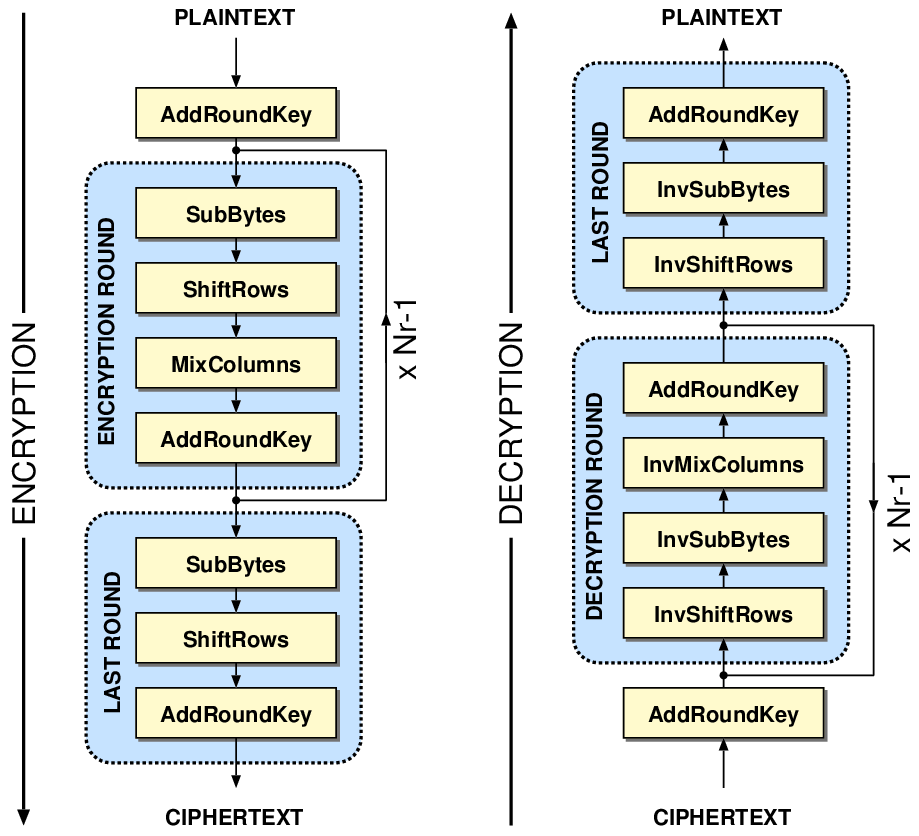
\includegraphics[width=0.55\textwidth]{images/AES.png}
    \caption[Internal AES behaviour]{Internal structure of the AES algorithm~\cite{imageAES}.}
    \label{fig:aes_rounds}
\end{figure}

\subsection{SubBytes}
The \textsc{SubBytes} operation is the only strictly non-linear transformation within the AES algorithm. 
It consists of a byte-by-byte substitution based on a fixed Look-Up Table (LUT) called the \textit{S-Box}. 
The S-Box is a $16 \times 16$ matrix containing every possible byte value, ranging from \texttt{0x00} to \texttt{0xFF}.

Both the columns and the rows are labeled in hexadecimal format from \texttt{0} to \texttt{F}. 
To apply the substitution, each byte of the State matrix is treated as a two-digit hexadecimal value: 
the first digit determines the row, and the second digit determines the column. 
The substituted byte is the value located at these intersecting coordinates.

\begin{figure}[htbp]
    \centering
    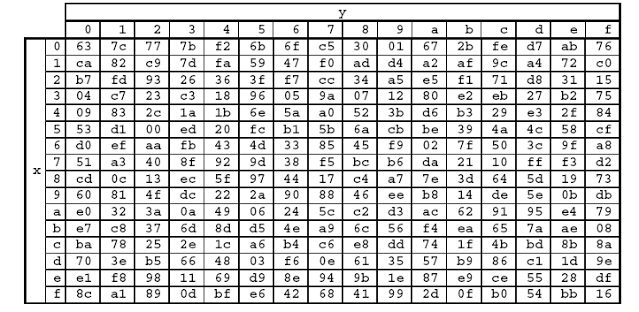
\includegraphics[width=1\textwidth]{images/Sbox.png}
    \caption[S-Box]{The AES Substitution Box (S-Box)~\cite{imageSBOX}.}
\end{figure}

For instance, considering the binary input $X = 01101100_2$, its hexadecimal representation is \texttt{0x6C}. 
By intersecting row \texttt{6} and column \texttt{C} in the S-Box, the output is \texttt{0x50}. 
Therefore, $\textsc{SubBytes}(\texttt{0x6C}) = \texttt{0x50}$.

\paragraph{The Construction of the S-Box}
The design of the S-Box stems from the fundamental cryptographic necessity to introduce strong non-linearity (confusion) into the cipher, 
rendering it highly resistant to linear and differential cryptanalysis. 

To achieve this, the S-Box is constructed through two mathematical steps. First, each element is mapped to its multiplicative inverse in the finite Galois Field $\mathrm{GF}(2^8)$. 
The multiplicative inverse $x^{-1}$ of a value $x$ in this finite field is defined as the value that, when multiplied by $x$, yields 1:
\begin{equation}
    x \cdot x^{-1} \equiv 1 \pmod{x^8 + x^4 + x^3 + x + 1}
    \label{eq:aes_field_inverse}
\end{equation}
The irreducible polynomial $x^8 + x^4 + x^3 + x + 1$ corresponds to the binary sequence $100011011_2$. 
This specific polynomial was selected by the AES creators to ensure the output is strictly constrained within an 8-bit length. 
By definition, the inverse of \texttt{0x00} is mapped to itself.

Secondly, to break algebraic symmetries and prevent structural attacks, each multiplicative inverse $b$ undergoes a specific affine transformation over $\mathrm{GF(2^8)}$: 
\[
b' = (A \cdot b) \oplus c
\]
where $A$ is a fixed $8 \times 8$ bit matrix, and $c$ is the constant column vector $[1,1,0,0,0,1,1,0]^T$ (corresponding to \texttt{0x63}).

\paragraph{Vulnerability of the Software LUT Implementation}
Because dynamically calculating the multiplicative inverse in $\mathrm{GF}(2^8)$ during every round would introduce an enormous computational overhead, 
standard software implementations, such as the \texttt{tiny-aes-c} library or those deployed on resource-constrained IoT and edge devices, 
rely entirely on precalculating these transformations and storing them in a static S-Box LUT.

Consequently, the necessity for these constrained devices to repeatedly access the LUT stored in memory or cache generates a deterministic physical energy leakage during each substitution. 
This power footprint is directly correlated with the specific byte value being processed, creating a vulnerability that can be readily exploited in Power Analysis Side-Channel Attacks.

Conversely, modern high-performance processors mitigate this vulnerability by utilizing dedicated cryptographic hardware extensions (e.g., Intel AES-NI or ARM CE). 
These hardware modules execute AES transformations directly within the CPU using dedicated logic gates, thereby eliminating the need for memory-based LUT lookups and effectively neutralizing this specific class of side-channel leakage.
However, such dedicated hardware extensions are rarely available on ultra-constrained embedded microcontrollers or legacy space-grade processors.

\subsection{ShiftRows}
The \textsc{ShiftRows} transformation is a linear operation primarily responsible for introducing horizontal diffusion across the State matrix. 
It adheres to the following mathematical formulation:

\begin{equation}
    s'_{r,c} = s_{r,(c+r) \bmod 4} \quad \text{for } 0 \le r < 4 \text{ and } 0 \le c < 4
    \label{eq:shift_rows}
\end{equation}

Following the application of \textsc{ShiftRows}, the resulting $4 \times 4$ matrix is altered such that the first row remains completely untouched. 
The second, third, and fourth rows undergo a cyclic left shift of one, two, and three byte positions, respectively. 

\[
S = \begin{bmatrix}
    s_{0,0} & s_{0,1} & s_{0,2} & s_{0,3} \\
    s_{1,0} & s_{1,1} & s_{1,2} & s_{1,3} \\
    s_{2,0} & s_{2,1} & s_{2,2} & s_{2,3} \\
    s_{3,0} & s_{3,1} & s_{3,2} & s_{3,3}
\end{bmatrix}
\xrightarrow{\quad \textsc{ShiftRows} \quad}
S' = \begin{bmatrix}
    s_{0,0} & s_{0,1} & s_{0,2} & s_{0,3} \\
    s_{1,1} & s_{1,2} & s_{1,3} & s_{1,0} \\
    s_{2,2} & s_{2,3} & s_{2,0} & s_{2,1} \\
    s_{3,3} & s_{3,0} & s_{3,1} & s_{3,2}
\end{bmatrix}
\]

While mechanically straightforward, this transformation is cryptographically vital. By shifting the rows, it ensures that the four bytes originally comprising a single column are distributed evenly across four distinct columns. 
Consequently, when the subsequent \textsc{MixColumns} transformation is applied, it will mathematically mix bytes from different original columns, guaranteeing a rapid and robust propagation of the avalanche effect throughout the entire State.

\subsection{MixColumns}
Complementing the horizontal diffusion introduced by \textsc{ShiftRows}, the \textsc{MixColumns} transformation is the primary operation responsible for applying vertical diffusion across the State matrix. 
This function ensures that each output byte in a column is mathematically dependent on every input byte within that same column.

To achieve this, each column is treated as a four-term polynomial and multiplied by a fixed matrix over the Galois Field $\mathrm{GF}(2^8)$:

\begin{equation}
\begin{bmatrix}
    s'_{0,c} \\
    s'_{1,c} \\
    s'_{2,c} \\
    s'_{3,c}
\end{bmatrix}
=
\begin{bmatrix}
    \texttt{02} & \texttt{03} & \texttt{01} & \texttt{01} \\
    \texttt{01} & \texttt{02} & \texttt{03} & \texttt{01} \\
    \texttt{01} & \texttt{01} & \texttt{02} & \texttt{03} \\
    \texttt{03} & \texttt{01} & \texttt{01} & \texttt{02}
\end{bmatrix}
\begin{bmatrix}
    s_{0,c} \\
    s_{1,c} \\
    s_{2,c} \\
    s_{3,c}
\end{bmatrix}
\quad \text{for } 0 \le c < 4
\label{eq:mix_columns_matrix}
\end{equation}

By expanding the matrix multiplication, where $\bullet$ denotes multiplication in $\mathrm{GF}(2^8)$ and $\oplus$ denotes bitwise XOR (addition in $\mathrm{GF}(2^8)$), the individual bytes of the new column are calculated as follows:

\begin{equation}
\begin{aligned}
    s'_{0,c} &= (\texttt{02} \bullet s_{0,c}) \oplus (\texttt{03} \bullet s_{1,c}) \oplus s_{2,c} \oplus s_{3,c} \\
    s'_{1,c} &= s_{0,c} \oplus (\texttt{02} \bullet s_{1,c}) \oplus (\texttt{03} \bullet s_{2,c}) \oplus s_{3,c} \\
    s'_{2,c} &= s_{0,c} \oplus s_{1,c} \oplus (\texttt{02} \bullet s_{2,c}) \oplus (\texttt{03} \bullet s_{3,c}) \\
    s'_{3,c} &= (\texttt{03} \bullet s_{0,c}) \oplus s_{1,c} \oplus s_{2,c} \oplus (\texttt{02} \bullet s_{3,c})
\end{aligned}
\label{eq:mix_columns_bytes}
\end{equation}

\paragraph{Software Implementation of GF($2^8$) Multiplication: xtime macro}
From a practical engineering perspective, performing heavy polynomial multiplications dynamically during every round would be computationally prohibitive for embedded systems. 
However, the matrix coefficients were deliberately selected by the AES designers to be exceptionally small (\texttt{01}, \texttt{02}, and \texttt{03}) to allow for radical software optimization. 

In lightweight C implementations such as \texttt{tiny-aes-c}, multiplication by \texttt{02} in $\mathrm{GF}(2^8)$ is elegantly implemented using a macro function typically named \texttt{xtime}. 
This operation consists of a simple bitwise left shift of the byte, followed by a conditional XOR with the irreducible polynomial \texttt{0x1B} if the most significant bit prior to the shift was 1. 

To rigorously verify this optimization, the generic input byte must be represented as a polynomial:
\[
A(x) = a_7x^7 + a_6x^6 + a_5x^5 + a_4x^4 + a_3x^3 + a_2x^2 + a_1x + a_0
\]
where the coefficients $a_7, \dots, a_0$ are individual bits, with $a_7$ being the Most Significant Bit (MSB).

The hexadecimal value \texttt{0x02} corresponds to the binary string \texttt{00000010}, which is equivalent to the polynomial $x$. 
Therefore, multiplying $A(x)$ by \texttt{0x02} yields:
\[
A(x) \cdot x = a_7x^8 + a_6x^7 + a_5x^6 + a_4x^5 + a_3x^4 + a_2x^3 + a_1x^2 + a_0x
\]
In computer architecture, multiplying by 2 corresponds exactly to a logical bitwise left shift of one position. 
However, to ensure the result remains within the finite field $\mathrm{GF}(2^8)$, the maximum degree of the resulting polynomial must not exceed $x^7$. 
This constraint presents two possible cases:

\begin{itemize}
    \item \textbf{$a_7 = 0$:} After the multiplication, the coefficient of $x^8$ is 0. The highest degree remains $x^7$, and no further mathematical reduction is necessary.
    
    \item \textbf{$a_7 = 1$:} The resulting polynomial contains an $x^8$ term, thus falling outside the finite field. 
    To bring the result back into $\mathrm{GF}(2^8)$, it must be divided by the AES irreducible polynomial ($x^8 + x^4 + x^3 + x + 1$), and replaced by the remainder of this division. 
    In binary arithmetic over $\mathrm{GF}(2)$, this modulo reduction corresponds precisely to an XOR operation with the irreducible polynomial:
    \[
    (A(x) \cdot x) \oplus (x^8 + x^4 + x^3 + x + 1)
    \]
\end{itemize}

Building on this logic, multiplication by \texttt{03} is effortlessly computed. 
Since \texttt{0x03} corresponds to the binary \texttt{00000011} (the polynomial $x + 1$), the multiplication $A(x) \cdot \texttt{0x03}$ expands to:
\[
A(x) \cdot (x + 1) = (A(x) \cdot x) + (A(x) \cdot 1) = (A(x) \cdot x) + A(x) 
\]
The first term, $(A(x) \cdot x)$, is exactly the \texttt{02} multiplication (\texttt{xtime}) just demonstrated. 
Meanwhile, polynomial addition in $\mathrm{GF}(2^8)$ is mathematically equivalent to a simple bitwise XOR. Thus, the operation seamlessly translates to $(\texttt{02} \bullet A) \oplus A$.

This architectural design guarantees that the \textsc{MixColumns} transformation remains exceptionally fast and highly efficient, 
relying strictly on basic CPU bitwise operations without necessitating additional memory-heavy LUTs.

\subsection{AddRoundKey}
The \textsc{AddRoundKey} transformation is the first operation applied in the algorithm. 
It consists of a straightforward bitwise XOR operation between the current \textit{State matrix} and the four words of the \textit{expanded key} corresponding to the current round.

For a given column $c$ (where $0 \le c < 4$) and a specific round, the transformation is defined as:
\[
\begin{bmatrix} s'_{0,c} \\ s'_{1,c} \\ s'_{2,c} \\ s'_{3,c} \end{bmatrix} 
= 
\begin{bmatrix} s_{0,c} \\ s_{1,c} \\ s_{2,c} \\ s_{3,c} \end{bmatrix} 
\oplus 
\begin{bmatrix} w_{4 \cdot \text{round} + c} \end{bmatrix}
\]

Consider, for instance, the application of the \textsc{AddRoundKey} transformation to the first column of the state ($c = 0$) during the first round. 
Let the initial state column and the corresponding word from the expanded key array ($w_4$) be defined as follows:
\[
\begin{bmatrix} 
    s_{0,0} \\ 
    s_{1,0} \\ 
    s_{2,0} \\ 
    s_{3,0} 
\end{bmatrix} 
= 
\begin{bmatrix} 
    \texttt{04} \\ 
    \texttt{E0} \\ 
    \texttt{48} \\ 
    \texttt{28} 
\end{bmatrix}
\qquad \text{and} \qquad
w_{4 \cdot 1 + 0} = w_4 = 
\begin{bmatrix} 
    \texttt{D6} \\ 
    \texttt{AA} \\ 
    \texttt{74} \\ 
    \texttt{FD} 
\end{bmatrix}
\]

By applying the bitwise XOR ($\oplus$) between the two column vectors, the resulting updated state column is computed as:

\begin{equation}
\begin{bmatrix} 
    s'_{0,0} \\ 
    s'_{1,0} \\ 
    s'_{2,0} \\ 
    s'_{3,0} 
\end{bmatrix} 
= 
\begin{bmatrix} 
    \texttt{04} \\ 
    \texttt{E0} \\ 
    \texttt{48} \\ 
    \texttt{28} 
\end{bmatrix} 
\oplus 
\begin{bmatrix} 
    \texttt{D6} \\ 
    \texttt{AA} \\ 
    \texttt{74} \\ 
    \texttt{FD} 
\end{bmatrix}
=
\begin{bmatrix} 
    \texttt{D2} \\ 
    \texttt{4A} \\ 
    \texttt{3C} \\ 
    \texttt{D5} 
\end{bmatrix}
\end{equation}

\section{Galois/Counter Mode (GCM)}
To apply a fixed-size block cipher such as AES to variable-length inputs, it is necessary to employ a specific \textit{mode of operation}. 
A mode of operation dictates the exact architectural procedure by which the core encryption algorithm processes data streams larger than its native 128-bit block size.

For instance, the most rudimentary mode of operation, \textit{Electronic Codebook (ECB)}~\cite[p. 9]{ECB_CTR}, starts by evaluating whether the plaintext length is an exact multiple of 128 bits.
If it is not, a padding scheme must be appended to the end of the message. The plaintext is then partitioned into 128-bit blocks, and each block is independently fed into the AES encryption algorithm. 
Finally, the resulting encrypted blocks are sequentially concatenated to form the complete ciphertext.

However, the ECB mode is notoriously vulnerable to cryptanalysis. Because the encryption of each block is entirely independent and deterministic, two identical plaintext blocks encrypted under the same key will invariably produce the exact same ciphertext blocks. 
This fatal flaw fails to eliminate large-scale redundancies, preserving the structural patterns of the original data and rendering it cryptographically inadequate for secure communications. 

To address these deterministic flaws, more advanced modes of operation were developed, such as the \textit{Counter Mode (CTR)}~\cite[p. 15--16]{ECB_CTR}. 
Unlike ECB, the CTR mode does not feed the plaintext directly into the cipher. Instead, it utilizes a 128-bit block comprising a unique \textit{nonce} (Number Used Once) concatenated with an internal counter.

In this architecture, the input to the AES algorithm is the counter block itself. 
The output of the AES encryption (a pseudo-random key stream) is then directly XORed with the current block of the plaintext to produce the ciphertext. 
For each subsequent block of the message, the value of the counter is incremented by one, encrypted by the block cipher, and XORed with the next plaintext block.
This operation is repeated until the entire message is processed.

The utilization of the counter as the AES input, instead of the plaintext block itself, guarantees the CTR mode a complete lack of inter-block dependency, representing a major architectural advantage.

By leveraging the possibility of pre-calculating the sequence of values that the counter will assume, the AES encryption operations can be highly parallelized, 
thereby achieving significantly higher throughput compared to sequential modes.

Although the baseline \texttt{tiny-aes-c} library~\cite{tinyAES} does not natively provide a GCM implementation, utilizing this specific mode is mandatory to accurately replicate the cryptographic environment characteristic of modern SATCOM systems. 
Consequently, as a core experimental contribution of this study, the GCM architecture was custom-implemented on top of the existing block cipher. 
This development was executed by strictly adhering to the official guidelines and mathematical specifications defined in NIST SP 800-38D~\cite{GCM}.

\paragraph{The GCM Extension: Authenticated Encryption and Integrity}
Building upon the architecture of the CTR mode, the \textit{Galois/Counter Mode (GCM)} expands the cryptographic framework by incorporating a robust authentication layer to ensure the integrity of the transmitted message. 
To achieve this, GCM implements an \textit{Authenticated Encryption with Associated Data (AEAD)} scheme.

In a typical network transmission, certain information must remain in plaintext to allow routers and gateways to correctly handle the packets. 
This is defined as the \textit{Additional Authenticated Data (AAD)}. 
The AAD typically comprises essential metadata such as network addresses, protocol versions, routing ports, and sequence numbers. 
The inclusion of sequence numbers is particularly critical in SATCOM environments to prevent \textit{replay attacks}, a severe threat involving the malicious interception and subsequent retransmission of a previously valid message.

While the AAD is transmitted unencrypted, its content, alongside the encrypted ciphertext, is mathematically processed by the algorithm to generate a unique 128-bit \textit{authentication tag}. 

During transmission, this authentication tag is appended to the message payload (which consists of the AAD and the ciphertext). 
Upon reception, the receiver replicates the exact same cryptographic process using the shared secret key, the received AAD, and the ciphertext to produce a new, localized authentication tag. 
If this locally generated tag perfectly matches the received tag, the receiver can safely conclude that neither the ciphertext nor the plaintext metadata was altered, corrupted, or tampered with during transmission.


\subsection{Key and IV Requirements}
While the standard CTR mode utilizes a unique nonce as the prefix for its counter, the GCM architecture delegates this critical role to the \textit{Initialization Vector (IV)}. 
To guarantee the designed cryptographic security bounds, strict regulatory requirements regarding the selection and management of both the key and the IV must be satisfied.

\paragraph{Uniqueness and Forgery Attacks.}
The most critical constraint of AES-GCM is the \textit{uniqueness requirement}. The standard dictates that the probability of the authenticated encryption function being invoked with the same Key/IV pair on two distinct plaintexts must be strictly less than $2^{-32}$. 

The consequences of violating this requirement by reusing an IV with the same key are catastrophic. By construction, the GHASH authentication tag is derived via polynomial evaluations over $\mathrm{GF}(2^{128})$ involving the ciphertext and the IV. 
If an IV is repeated, an attacker can mathematically recover the internal authentication subkey. This exposes the system to \textit{forgery attacks}, allowing the attacker to produce fake messages with valid authentication tags, completely compromising the integrity of the channel. 
In practice, safeguarding IV uniqueness is considered as vital as maintaining the secrecy of the master key itself.

\paragraph{Key Freshness and Establishment.}
In addition to the IV, key management plays a pivotal role. The principles of \textit{key uniqueness} and \textit{key establishment} mandate that for each new communication session, the generated symmetric key must be ``fresh'' (cryptographically unpredictable). 
Furthermore, the communication channel utilized to distribute this master key (often asymmetric or out-of-band) must be highly secure to prevent key theft prior to the AES-GCM execution.

\paragraph{IV Construction Methods.}
Because of the vital role the IV plays, NIST SP 800-38D~\cite{GCM} outlines strict construction rules, heavily recommending a standard IV length of 96 bits for optimal performance and security. 
Depending on the system architecture, two main generation processes are defined:

\begin{itemize}
    \item \textbf{Deterministic Construction:} This method is mandatory for IVs strictly shorter than 96 bits, but is widely used for 96-bit IVs as well. 
    It stipulates that the IV is divided into two sections: a \textit{fixed field} and an \textit{invocation field}. 
    The fixed field uniquely identifies the device or the specific instance of the encryption algorithm (e.g., a satellite ID), whereas the invocation field acts as a sequential counter for the data sets. 
    To maintain uniqueness, two devices sharing the same key must never share the same fixed field, and the invocation field must increment deterministically.
    
    \item \textbf{RBG-based Construction:} For IVs of 96 bits or longer, a \textit{Random Bit Generator (RBG)} construction can be employed. 
    This format consists of a \textit{random field} and an optional \textit{free field}. 
    To satisfy the $2^{-32}$ collision probability threshold, the random field must have a minimum length of 96 bits and be generated by a cryptographically strong RBG. 
    The free field has no structural requirements and can contain arbitrary device metadata, though the standard suggests leaving it empty to maximize the entropy of a fully randomized IV.
\end{itemize}

\subsection{Multiplication in \texorpdfstring{$\mathrm{GF}(2^{128})$}{GF(2\textasciicircum 128)}}
As previously introduced in the \textsc{MixColumns} analysis, calculations within Galois Finite Fields are utilized to guarantee mathematical closure and strong diffusion, 
ensuring that outputs remain strictly within a defined range while maintaining the influence of every input bit. 
Correspondingly, one of the primary mathematical operations underlying the GCM authenticated encryption scheme is Galois multiplication applied over the extended finite field $\mathrm{GF}(2^{128})$.

Within $\mathrm{GF}(2^{128})$, 128-bit blocks are treated as polynomials with a maximum degree of 127. 
Each bit of the data block represents the coefficient of the corresponding polynomial term, ranging from $x^0$ to $x^{127}$.

\begin{algorithm}[htbp]
\caption{Multiplication in $\mathrm{GF}(2^{128})$: $X \bullet Y$}
\label{alg:gf128_mult}
\begin{algorithmic}[1]
\Procedure{galoisMultiplication}{$X, Y$}
    \State $R \gets 11100001_2 \,\|\, 0^{120}$
    \State $Z \gets 0^{128}$
    \State $V \gets Y$
    \For{$i \gets 0$ \textbf{to} $127$}
        \If{$x_i = 1$} \Comment{$x_i$ is the $i$-th bit of block $X$}
            \State $Z \gets Z \oplus V$
        \EndIf
        \If{$\text{LSB}_1(V) = 0$}
            \State $V \gets (V \gg 1$)
        \Else
            \State $V \gets (V \gg 1) \oplus R$
        \EndIf
    \EndFor
    \State \Return $Z$
\EndProcedure
\end{algorithmic}
\end{algorithm}

The algorithmic translation of this multiplication logic begins with the initialization of three primary variables \texttt{(lines 2--4)}:
\begin{itemize}
    \item $R$: Represents the reduction polynomial block, which is used to bring the result back into the finite field whenever a polynomial multiplication exceeds the maximum degree constraint. 
    The formal irreducible polynomial chosen by the GCM designers is $f(x) = x^{128} + x^7 + x^2 + x + 1$. 
    During modulo reduction in $\mathrm{GF}(2^{128})$, the $x^{128}$ term is mathematically substituted by $x^7 + x^2 + x + 1$. 
    Following the NIST SP 800-38D standard~\cite{GCM}, which adopts a \textit{bit-reflected} convention, operating analogously to a little-endian scheme, where the leftmost bit is interpreted as the $x^0$ coefficient, this reduction polynomial is mapped to the binary string $11100001_2 \,\|\, 0^{120}$ (equivalent to the hexadecimal block \texttt{0xE100...00}).
    
    \item $Z$: The accumulator variable, initialized as an array of 128 zeros ($0^{128}$).
    
    \item $V$: The multiplicand variable, initialized as a direct copy of the input block $Y$.
\end{itemize}

To calculate the product $X \bullet Y$ in $\mathrm{GF}(2^{128})$, the algorithm employs a process known as \textit{Shift-and-Add}, which mathematically mirrors classical column-wise multiplication. 

Considering that the 128-bit block $X$ is treated as a polynomial with a maximum degree of 127:
\[
X = x_0 + x_1x + x_2x^2 + \dots + x_{127}x^{127}
\]
by applying the distributive property, the multiplication between $X$ and $Y$ can be expanded as follows (where modulo 2 addition is logically equivalent to the bitwise XOR operator $\oplus$):
\[
X \bullet Y = (x_0 \cdot Y) \oplus (x_1 \cdot Y \cdot x) \oplus (x_2 \cdot Y \cdot x^2) \oplus \dots \oplus (x_{127} \cdot Y \cdot x^{127})
\]

Within the algorithm's pseudocode, this mathematical expansion is implemented inside the main loop \texttt{(lines 5--14)}. 
The execution of each iteration can be broken down into two distinct operational phases: the accumulation phase and the shift-and-reduce phase.

\paragraph{Phase 1: Accumulation (Lines 6--8)}
During the $i$-th iteration, the algorithm inspects the state of $x_i$ (the $i$-th bit of $X$) to determine its contribution to the final product:
\begin{itemize}
    \item \textbf{If $x_i = 1$:} The mathematical term evaluates to $Y \cdot x^i$. Consequently, the current value of the multiplicand $V$ (which currently holds the value $Y \cdot x^i$) is XORed into the accumulator $Z$ \texttt{(line 7)}.
    \item \textbf{If $x_i = 0$:} The term evaluates to $0$. Since zero is the identity element for the XOR operation, it acts as a null term, and the accumulator $Z$ remains unchanged.
\end{itemize}

\paragraph{Phase 2: Shift and Reduce (Lines 9--13)}
In the final phase of the iteration, the state of the multiplicand $V$ must be updated for the next loop by multiplying it by $x$ (effectively elevating its polynomial degree). 
Crucially, because the NIST SP 800-38D standard mandates a \textit{bit-reflected} (little-endian) convention, elevating the polynomial degree corresponds to a \textbf{logical right shift} ($\gg 1$) at the architectural level, rather than a traditional left shift.

Moreover, to guarantee that the temporary result remains strictly within the $\mathrm{GF}(2^{128})$ boundaries, a boundary check is executed on the highest degree coefficient prior to the shift \texttt{(line 9)}. 
Due to the bit-reflected nature of the data, the highest degree coefficient ($x^{127}$) is physically located at the Least Significant Bit ($\text{LSB}_1$) of the array. 
If this bit is 0, a simple right shift is sufficient. However, if the LSB is 1, the subsequent right shift would cause an overflow outside the finite field. 
To mathematically correct this, the shifted result is immediately XORed with the irreducible polynomial $R$ \texttt{(line 12)}, seamlessly reducing the value back into the valid finite field space.

\paragraph{Additional Challenges of GCM}
As highlighted in the section detailing the S-Box substitution, executing repeated algebraic operations natively within a Galois Field (in this case, $\mathrm{GF}(2^{128})$ for the GHASH multiplication) imposes a significant computational and energetic overhead. 
This mathematical burden is often incompatible with the strict power budgets of resource-constrained devices, such as space-segment satellite components.

To address this critical efficiency bottleneck, these embedded architectures typically adopt a structural compromise remarkably similar to the S-Box implementation: leveraging pre-computed Look-Up Tables (LUTs). 
Specifically, Shoup's method or the 4-bit table-driven approach~\cite{Shoup} pre-calculates the polynomial multiplications, allowing the device to perform the GCM authentication via fast memory lookups and XOR operations rather than dynamic arithmetic. 
Alternatively, modern architectures might utilize dedicated hardware instructions (such as the \texttt{PCLMULQDQ} instruction in x86 environments)~\cite{PCLMULQDQ} to perform carry-less multiplications directly in the silicon logic, minimizing the energy-per-bit cost while bypassing the memory constraints.


\subsection{\texorpdfstring{$\text{GHASH}$}{GHASH} Function}
The generation of the authentication tag is the theoretical core of the GCM architecture, and the $\text{GHASH}$ function serves as the mathematical engine utilized by the main encryption algorithm to achieve this integrity guarantee.

Despite its name, $\text{GHASH}$ is not a traditional unkeyed cryptographic hash function (such as SHA-256), but rather a \textit{universal hash function}. 
It is specifically designed to compute a 128-bit message authentication code (MAC) by evaluating a polynomial over $\mathrm{GF}(2^{128})$. 
When combined with the strict IV uniqueness requirements, it provides an extremely low probability of differential output collisions. 

The cornerstone of the $\text{GHASH}$ design is the utilization of the \textit{hash subkey} $H$. 
This subkey is derived by applying the block cipher to a 128-bit block of zeros under the master key, meaning $H = \text{AES}_K(0^{128})$. 
Ultimately, the core operation executed within this function is the \textsc{galoisMultiplication} previously defined, which processes the data blocks iteratively.

\begin{algorithm}[htbp]
\caption{$\text{GHASH}_H$ Function}
\label{alg:ghash}
\begin{algorithmic}[1]
\Procedure{$\text{GHASH}_H$}{$X$}
    \State $m \gets \text{len}(X) / 128$
    \State Let $X_1, X_2, \dots, X_m$ denote the blocks such that $X = X_1 \,\|\, X_2 \,\|\, \dots \,\|\, X_m$
    \State $Y \gets 0^{128}$
    \For{$i \gets 1$ \textbf{to} $m$}
        \State $Y \gets \textsc{galoisMultiplication}(Y \oplus X_i, H)$ \Comment{Multiplication in $\mathrm{GF}(2^{128})$}
    \EndFor
    \State \Return $Y$
\EndProcedure
\end{algorithmic}
\end{algorithm}

As detailed in Algorithm~\ref{alg:ghash}, the variable $m$ denotes the total number of 128-bit blocks comprising the input $X$ \texttt{(line 2)}. 
The sequence $X_1, X_2, \dots, X_m$ represents each sequential 128-bit section of the input \texttt{(line 3)}, 
followed by the initialization of $Y$, a zero-block utilized as the accumulator variable \texttt{(line 4)}. 
Finally, for each $i$-th block $X_i$, the accumulator $Y$ is mathematically updated with the output of the Galois multiplication between the hash subkey $H$ and the XORed state of $Y \oplus X_i$.

\paragraph{Embedded C Implementation and Memory Optimization.}
In space-grade embedded systems, dynamically allocating memory (e.g., utilizing the heap via \texttt{malloc}) for variable-length inputs is strictly avoided to prevent memory fragmentation and ensure deterministic execution. 
Conversely, copying massive payloads directly onto the stack would immediately lead to stack overflow faults.

To address these severe architectural constraints within the \texttt{tiny-aes-c} extension~\cite{tinyAES}, the theoretical $\text{GHASH}$ algorithm was not implemented as a standalone function. 
Instead, the mathematical operations are executed \textit{in-place} inside the main authenticated encryption and decryption routines. 
As shown in the code snippet below, the implementation iteratively processes the Additional Authenticated Data (AAD) and the ciphertext in 16-byte chunks, XORing them directly into the accumulator \texttt{S} and immediately calling the \texttt{galoisMultiplication} function. 

\begin{clisting}[label={lst:ghash_inline}]{In-place GHASH memory optimization loop.}
// Processing AAD in blocks of 16 bytes without dynamic memory allocation
for (size_t i = 0; i < aad_length; i += AES_BLOCKLEN) {
    for (size_t j = 0; j < AES_BLOCKLEN; j++) {
        if (i + j < aad_length) {
            S[j] ^= aad[i + j];
        }
    }
    galoisMultiplication(S, H, S);
}
\end{clisting}

This engineering approach entirely circumvents the need to duplicate large data structures in memory, rigorously adapting the high-level NIST specifications to the harsh constraints of lightweight satellite microcontrollers.

\subsection{Authenticated Encryption and Decryption Algorithms}
Ultimately, all the cryptographic primitives and modes of operation detailed in this chapter converge into the final Authenticated Encryption with Associated Data (AEAD) algorithms. 
These procedures orchestrate the encryption process to produce a secure ciphertext accompanied by an authentication tag, and conversely, manage the decryption process while cryptographically verifying the message's authenticity through tag comparison.

\paragraph{Authenticated Encryption Algorithm}
The encryption algorithm operates on the following set of input variables:
\begin{itemize}
    \item $K$: The secret 256-bit \textit{master key}.
    \item $IV$: The variable-length \textit{Initialization Vector}, chosen in accordance with official NIST specifications~\cite[p. 18--21]{GCM} (in modern SATCOM standards, this is conventionally fixed at 96 bits / 12 bytes).
    \item $P$: The variable-length input \textit{plaintext}.
    \item $A$: The \textit{Additional Authenticated Data (AAD)}.
    \item $t$: An integer value determining the maximum bit-length of the generated authentication tag.
\end{itemize}

Moreover, a set of auxiliary subroutines is utilized during execution. 
The $\textsc{Ciph}_K()$ routine invokes the core AES block cipher to encrypt a 128-bit zero-block, producing the hash subkey $H$. 
The $\text{inc}_{32}()$ function takes a 128-bit block and increments its 32 rightmost bits, which act as a counter that wraps around to zero upon overflow. 
Lastly, $\textsc{Gctr}_K()$ executes the standard CTR mode of operation for a fixed key $K$, processing a given input payload starting from a specified initial counter block.

\begin{algorithm}[htbp]
\small
\caption{GCM Authenticated Encryption}
\label{alg:gcm_ae}
\begin{algorithmic}[1]
\Procedure{GcmAuthenticatedEncrypt}{$K, IV, P, A, t$}
    \State $H \gets \textsc{Ciph}_K(0^{128})$ \Comment{Generate the hash subkey $H$}
    \If{$\text{len}(IV) = 96$}
        \State $J_0 \gets IV \,\|\, 0^{31} \,\|\, 1$
    \Else
        \State $s \gets 128 \cdot \lceil \text{len}(IV)/128 \rceil - \text{len}(IV)$
        \State $J_0 \gets \textsc{Ghash}_H(IV \,\|\, 0^{s+64} \,\|\, [\text{len}(IV)]_{64})$
    \EndIf
    \State $C \gets \textsc{Gctr}_K(\text{inc}_{32}(J_0), P)$ \Comment{Encrypt plaintext $P$}
    \State $u \gets 128 \cdot \lceil \text{len}(C)/128 \rceil - \text{len}(C)$
    \State $v \gets 128 \cdot \lceil \text{len}(A)/128 \rceil - \text{len}(A)$
    \State $S \gets \textsc{Ghash}_H(A \,\|\, 0^v \,\|\, C \,\|\, 0^u \,\|\, [\text{len}(A)]_{64} \,\|\, [\text{len}(C)]_{64})$
    \State $T \gets \text{MSB}_t(\textsc{Gctr}_K(J_0, S))$ \Comment{Compute authentication tag of length $t$}
    \State \Return $(C, T)$
\EndProcedure
\end{algorithmic}
\end{algorithm}

The procedure initiates by computing the hash subkey $H$ via the $\textsc{Ciph}_K()$ routine \texttt{(line 2)}. 
Subsequently, a conditional structure determines the format of the initial counter block $J_0$ \texttt{(lines 3--8)}. 
If the $IV$ is exactly 96 bits long, $J_0$ is constructed by concatenating the $IV$ with a 32-bit counter initialized to 1. 
Conversely, if the $IV$ length differs from 96 bits, an integer $s$ is calculated to determine the required zero-padding. 
The counter block $J_0$ is then generated by passing the $IV$, the zero-padding, and a 64-bit representation of the $IV$'s length through the $\textsc{Ghash}_H()$ function.

Following initialization, the ciphertext $C$ is produced using the $\textsc{Gctr}_K()$ routine, utilizing the incremented initial counter (which resolves to \texttt{02} for a 96-bit $IV$) and the plaintext $P$ as inputs \texttt{(line 9)}.

Continuing the process, two integer values, $u$ and $v$, are calculated to determine the required zero-padding based on the lengths of the ciphertext and the AAD, respectively \texttt{(lines 10--11)}. 
An intermediate accumulator block $S$ is then produced via the $\textsc{Ghash}_H()$ operation by evaluating the concatenation of the AAD, its padding, the ciphertext, its padding, and the 64-bit length representations of both the AAD and the ciphertext \texttt{(line 12)}. 
Ultimately, the authentication tag $T$ is generated by encrypting $S$ with the original initial counter $J_0$, extracting only the $t$ most significant bits \texttt{(line 13)}.

\begin{figure}[htbp]
    \centering
    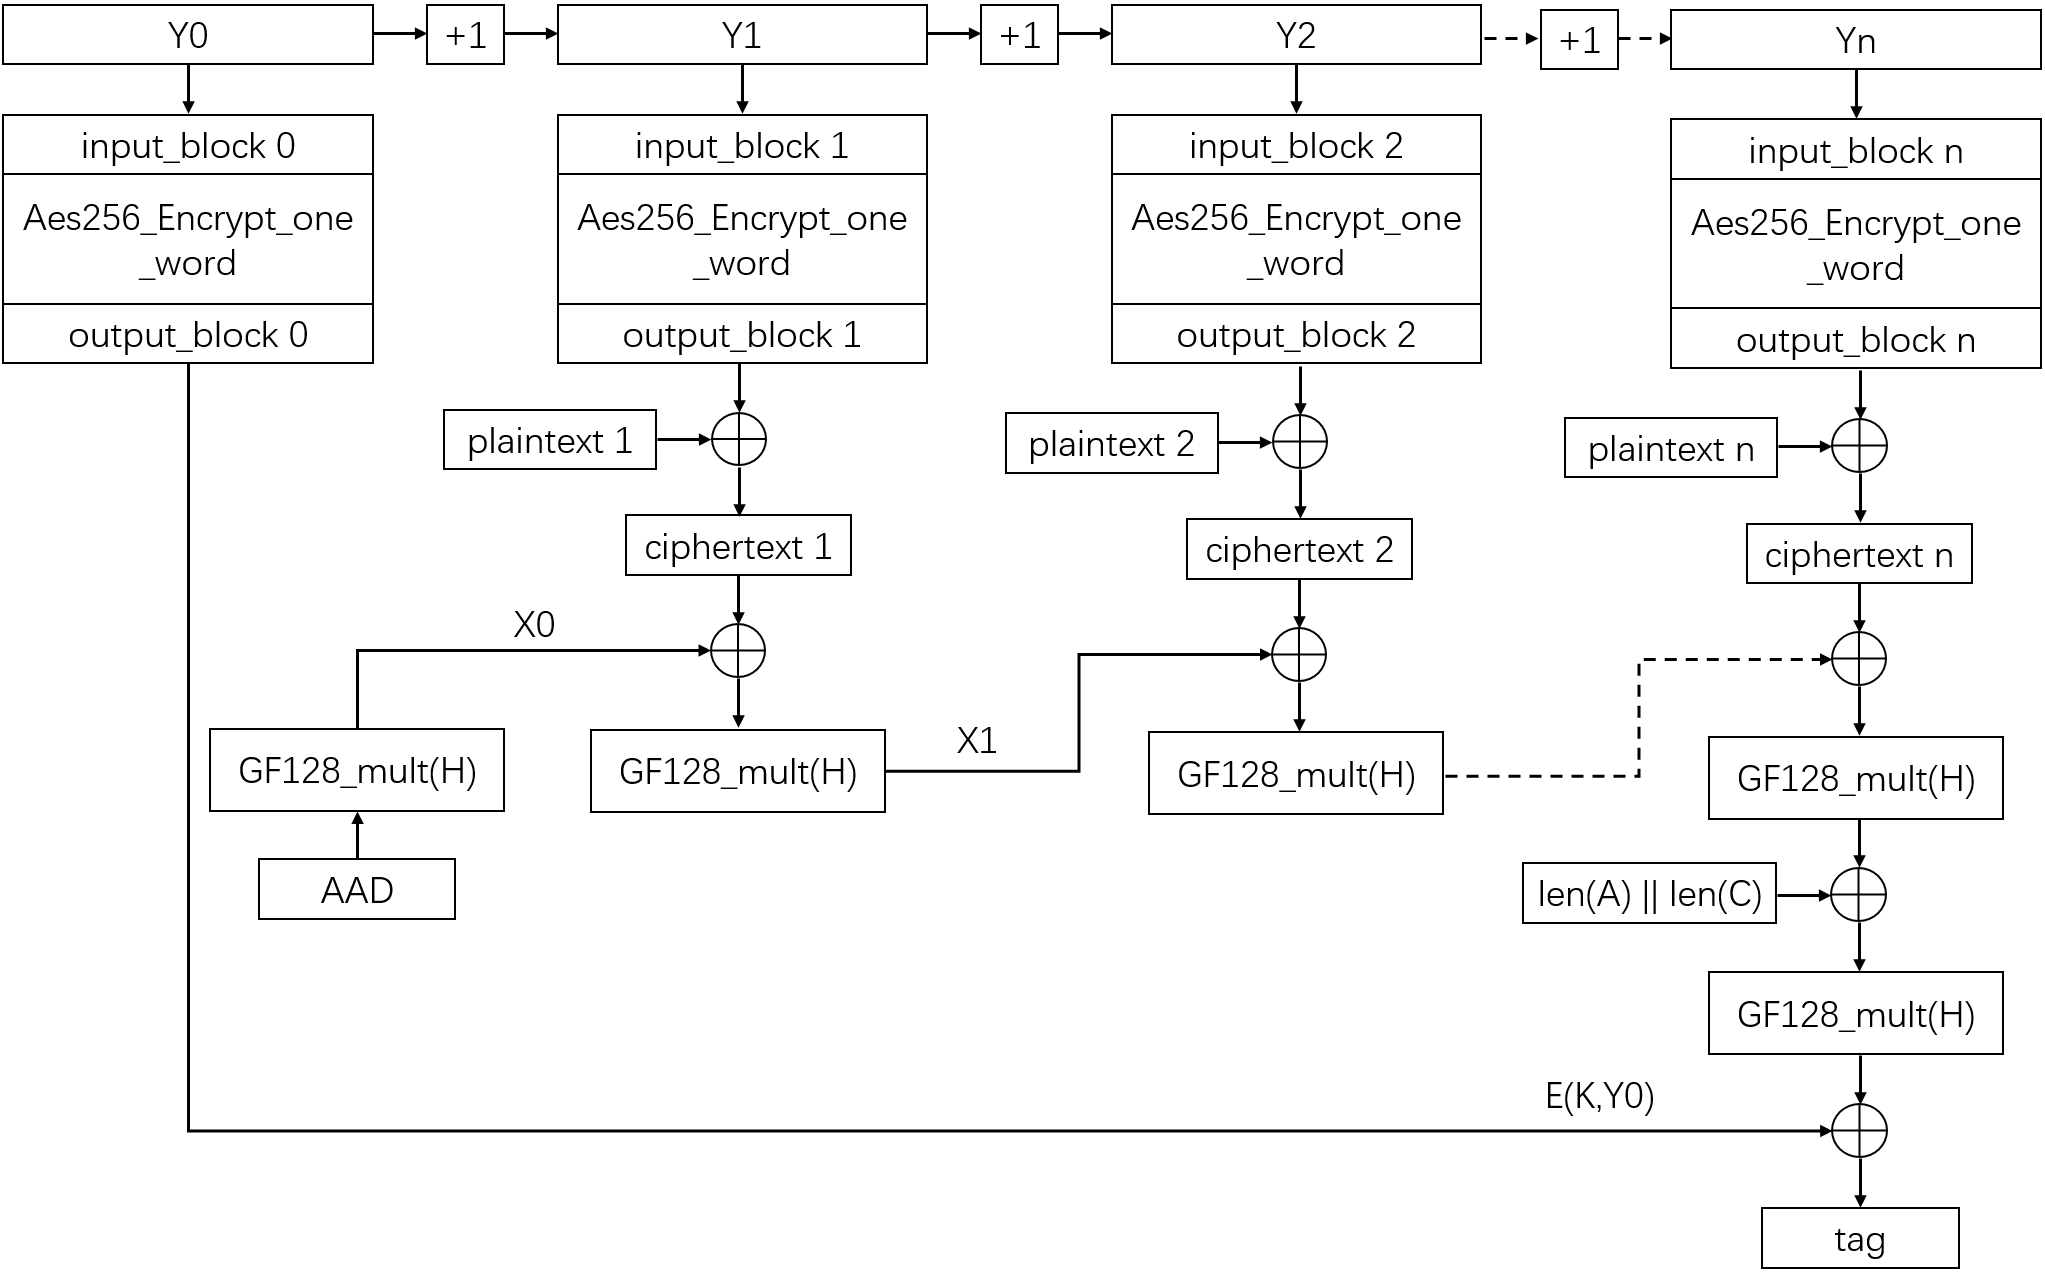
\includegraphics[width=0.78\textwidth]{images/GCM_encryption.png}
    \caption[AES-GCM Authenticated Encryption Scheme]{AES-GCM Authenticated Encryption architecture detailing the data flow and tag generation process~\cite{imageGCM}.}
    \label{fig:gcm_encryption_arch}
\end{figure}

\FloatBarrier

\paragraph{Authenticated Decryption Algorithm}
The authenticated decryption algorithm shares the vast majority of its cryptographic logic with its encryption counterpart. 
The primary operational differences reside in the initial validation checks, which verify that the bit-lengths of the $IV$, AAD, and ciphertext are supported, and that the provided tag matches the expected length $t$. 
Additionally, the transposition of the input variable $C$ (ciphertext) in place of $P$ (plaintext) represents a key difference.

Crucially, after following the standard computational flow to produce a localized tag $T'$, the algorithm executes a constant-time comparison between $T'$ and the received tag $T$. 
If the two tags match perfectly, the authentication succeeds, and the decrypted plaintext is released. 
Otherwise, the message is deemed compromised, either through malicious tampering or transmission errors. 
In this failure state, the algorithm immediately aborts and returns a $\textsc{Fail}$ error \texttt{(lines 19--20)}, strictly discarding the plaintext to prevent Chosen-Ciphertext Attacks (CCA).

\begin{algorithm}[H]
\footnotesize
\caption{GCM Authenticated Decryption}
\label{alg:gcm_ad}
\begin{algorithmic}[1]
\Procedure{GcmAuthenticatedDecrypt}{$K, IV, C, A, T, t$}
    \If{bit lengths of $IV, A$, or $C$ are unsupported \textbf{or} $\text{len}(T) \neq t$} \textbf{return} $\textsc{Fail}$ \EndIf
    \State $H \gets \textsc{Ciph}_K(0^{128})$ \Comment{Generate hash subkey $H$}
    \If{$\text{len}(IV) = 96$}
        \State $J_0 \gets IV \,\|\, 0^{31} \,\|\, 1$
    \Else
        \State $s \gets 128 \cdot \lceil \text{len}(IV)/128 \rceil - \text{len}(IV)$; \quad $J_0 \gets \textsc{Ghash}_H(IV \,\|\, 0^{s+64} \,\|\, [\text{len}(IV)]_{64})$
    \EndIf
    \State $P \gets \textsc{Gctr}_K(\text{inc}_{32}(J_0), C)$ \Comment{Decrypt ciphertext $C$}
    \State $u \gets 128 \cdot \lceil \text{len}(C)/128 \rceil - \text{len}(C)$; \quad $v \gets 128 \cdot \lceil \text{len}(A)/128 \rceil - \text{len}(A)$
    \State $S \gets \textsc{Ghash}_H(A \,\|\, 0^v \,\|\, C \,\|\, 0^u \,\|\, [\text{len}(A)]_{64} \,\|\, [\text{len}(C)]_{64})$
    \State $T' \gets \text{MSB}_t(\textsc{Gctr}_K(J_0, S))$ \Comment{Compute expected tag}
    \If{$T = T'$} \textbf{return} $P$ \Comment{Authentication succeeded}
    \Else\ \textbf{return} $\textsc{Fail}$ \Comment{Integrity check failed}
    \EndIf
\EndProcedure
\end{algorithmic}
\end{algorithm}


\subsection{Tests for the GCM Embedded C Implementation}

\paragraph{NIST Vector Tests}
To rigorously verify the cryptographic correctness of the custom C implementation, a selected suite of test vectors was utilized~\cite{vectorTests}. 
These test vectors are provided by the \textit{Cryptographic Algorithm Validation Program (CAVP)}, established directly by NIST. 

The suite contains tens of thousands of individual test cases for both the authenticated encryption and decryption processes. 
Each test evaluates the algorithm against variable-length plaintexts, ciphertexts, IVs, and AADs, utilizing diverse 256-bit master keys and their corresponding expected authentication tags. 

The execution of these tests yielded a 100\% success rate, demonstrating that the embedded implementation is mathematically sound and fully compliant with the FIPS and NIST standards.

\paragraph{Channel Noise and SEU Simulation}
Beyond formal cryptographic validation, a practical simulation was developed to replicate the effects of \textit{Additive White Gaussian Noise (AWGN)} and radiation-induced \textit{Single Event Upsets (SEUs)}, which represent critical concerns in SATCOM environments. 

It is vital to verify that the AEAD architecture correctly identifies arbitrary bit-level message alterations caused by the harsh space environment. 
To emulate a transmission error over a noisy channel, a random bit-flip was artificially injected into a valid ciphertext prior to the decryption phase. 

\begin{lightterminal}
Plaintext (429 byte): SAT-7 telemetry window 2041: the spacecraft is in nominal sun-pointing attitude and the Ka-band link remains locked with the ground station in Matera. The flight computer reports stable battery voltage, adequate thermal margins, and no corrected memory errors during the last pass. Payload data will be downlinked in two scheduled contact windows; the receiver shall request a repeat only if the authenticated packet check fails.
AAD (95 byte): SAT-7|pass=2041|ground-station=Matera|band=Ka|channel=telemetry|priority=nominal|counter=000184
Randomly flipped bit 1896 of the ciphertext.
Received Tag: 518735e4ea1697d3dcf9f0bb69ae65e4
ERROR: decryption failed as expected due to the bit flip.
\end{lightterminal}

\paragraph{Chaotic Injection overview}
With the baseline AES-256-GCM architecture fully implemented, theoretically analyzed, and functionally validated, the foundational framework of this study is established. 
The next chapter will address the physical vulnerabilities of this standard implementation by integrating a chaotic injection mechanism into the S-Box. 
Drawing inspiration from the foundational concepts proposed by Kumar et al.~\cite{KumarPaper}, the following chapter explores a cryptographic ``Machine Unlearning'' approach, deliberately adapting it to break the deterministic power leakages exploited by advanced ML-based Side-Channel Attacks in SATCOM environments.

% ====================================================================================================

% ====================================================================================================

\chapter[Chaotic Injection and Cryptographic Machine Unlearning]{Chaotic Injection and Cryptographic \\ Machine Unlearning}
In recent years, the widespread accessibility of Machine Learning (ML) has transformed it into a severe cryptographic threat. 
When utilized as a mechanism for advanced cryptanalysis, ML models, ranging from Deep Learning architectures to ensemble methods like Random Forests, 
can reduce the time required to mount successful attacks by several orders of magnitude, often rendering previously unfeasible exploits highly practical.

These data-driven techniques inherently rely on massive training datasets to identify underlying patterns. 
To achieve high classification accuracy, an ML model requires the target system's behavior to be strictly deterministic and stationary. 
In the context of secure SATCOMs, the physical implementation of the AES block cipher provides exactly this ideal environment for an attacker.

Crucially, while the AES \textsc{SubBytes} (S-Box) transformation is mathematically \textit{non-linear} to prevent algebraic attacks, its software execution typically relies on a static Look-Up Table (LUT). 
Consequently, processing a specific input byte will invariably execute the exact same memory access sequence, generating a deterministic physical leakage (e.g., power consumption). 
While this subtle leakage is nearly impossible to analyze manually, ML algorithms excel at mapping these stable physical traces back to the sensitive key bytes.

To neutralize this threat, this study builds upon the chaotic injection research proposed by Kumar et al.~\cite{KumarPaper}. 
Their work introduces a solution defined as a cryptographic \textit{Machine Unlearning} system. 
Rather than stripping data from an existing ML model, this approach injects dynamic, chaotic perturbations directly into the S-Box routine to proactively destroy the deterministic physical footprint.

\paragraph{Mathematical Modeling of the Chaotic S-Box}
According to the theoretical framework established by Kumar et al.~\cite[p. 161]{KumarPaper}, this cryptographic unlearning is governed by the chaotic evolution of a state variable $W(t)$. 
The evolution of this state across iterations is defined by the following equation:
\begin{equation}
    W(t+1) = W(t) + \alpha \cdot \Delta W - \beta \cdot |W(t)|
    \label{eq:chaotic_evolution}
\end{equation}
In this dynamic system, $\alpha$ represents the learning rate governing the chaotic perturbation, while $\beta$ acts as a crucial forgetting factor. 
The term $\beta$ physically dictates the rate at which the system ``forgets'' any previously stable structural patterns over time.

According to the original theoretical framework, the chaotic system forces the encryption algorithm to forget structured learning by continuously evolving an entire weight matrix. 
In this baseline model, each individual weight $w_{ij}$ within the matrix is iteratively updated via the following relation:
\begin{equation}
    w_{ij}^{(t+1)} = w_{ij}^{(t)} + \epsilon F_{chaos}(X_t)
    \label{eq:matrix_update}
\end{equation}
where $\epsilon$ acts as the chaos scaling factor, $X_t$ is the current chaotic variable at iteration $t$, and $F_{chaos}(X_t)$ represents a specific mathematical perturbation function. 

To effectively shield the AES algorithm, this evolving chaotic state $W(t)$ is injected into the substitution process. 
The resulting dynamic hybrid S-Box is mathematically modeled as:
\begin{equation}
    S'(x,t) = A \cdot x^{-1} \oplus C + \gamma \cdot \tanh(\delta \cdot W(t))
    \label{eq:chaotic_sbox}
\end{equation}
In this formulation, the first term $(A \cdot x^{-1} \oplus C)$ represents the standard AES affine transformation over $\mathrm{GF}(2^8)$, which ensures the necessary cryptographic diffusion and confusion. 
The second term introduces the chaotic modulation: $\gamma$ controls the absolute strength of the chaotic perturbation, and $\delta$ scales the sensitivity of the chaos. 
Finally, the hyperbolic tangent function ($\tanh$) is essential to ensure that the chaotic noise remains strictly bounded, preserving the algorithm's mathematical bijectivity and guaranteeing a correct decryption process.

\paragraph{Chaotic Influence on Key Expansion}
Furthermore, the injection of chaos is not strictly limited to the plaintext substitution phase. 
Because the AES Key Expansion algorithm internally relies on the S-Box during the \textsc{SubWord} routine to generate the 14 round keys, the dynamic chaotic state inherently propagates into the key schedule as well. 
This structural involvement implies that, in addition to the individual data bytes processed during standard encryption and decryption, the entire expanded key generation is continuously influenced by the chaotic perturbations, 
thereby significantly increasing the unpredictability of the cryptographic state.

\paragraph{Architectural Optimization: The Scalar Chaotic State}
While the theoretical framework proposed by Kumar et al.~\cite{KumarPaper} conceptualizes $W(t)$ as a multidimensional weight matrix to maximize theoretical entropy, continuously evaluating and updating an entire matrix introduces severe computational and memory overheads. 
Such complexity is inherently incompatible with the strict power budgets and memory limitations of lightweight SATCOM embedded systems.

To resolve this architectural bottleneck, this thesis introduces a critical optimization: the multidimensional matrix $W(t)$ is algorithmically collapsed into a single scalar chaotic variable. 
Crucially, this scalar state continues to evolve according to the fundamental unlearning dynamics defined in Equation~\ref{eq:chaotic_evolution}, thereby preserving the crucial role of the forgetting factor $\beta$.
As will be demonstrated through empirical testing, tracking and updating a scalar value provides sufficient non-linear entropy to successfully mask the S-Box power signature. 
Therefore, this custom implementation achieves the required cryptographic unlearning while rigorously preserving the efficiency dictated by the \texttt{tiny-aes-c}~\cite{tinyAES} baseline and space-grade microcontrollers.

Finally, in the theoretical model, the term $\Delta W$ in Equation~\ref{eq:chaotic_evolution} is broadly defined as the weight adjustment derived from the system's learning process. 
However, a symmetric block cipher like AES does not possess a traditional ML loss function or a backpropagation mechanism to calculate a literal ``learning'' gradient during the encryption phase.

To bridge this gap between ML theory and practical cryptography, this thesis explicitly redefines $\Delta W$ as the discrete differential of the chosen chaotic map. 
Specifically, for any given chaotic map generating a state sequence $X$, the adjustment is calculated as the exact difference between the updated state and the previous one ($\Delta W = X_{t+1} - X_t$). 
By doing so, the state evolution $W(t)$ is driven entirely by pure chaotic dynamics rather than simulated learning. 
This adaptation ensures deterministic reversibility, which is mandatory for decryption, while maximizing the unpredictable variation of the S-Box physical footprint.

\section{Taxonomy of the Implemented Chaotic Maps}
As detailed in~\cite[p. 7]{origineMappeCaotiche}, chaotic maps are mathematical functions characterized by an extreme sensitivity to initial conditions. 
When evaluated using specific chaos-optimal parameters, these functions generate a sequence of deterministic, yet highly unpredictable, state evolutions.

Although the cryptographic machine unlearning objective could theoretically be achieved utilizing any valid chaotic function, 
it is essential to evaluate a diverse taxonomy of maps to thoroughly analyze their behavioral properties. 
Chaotic maps differ significantly in their mathematical construction, primarily distinguished by their dimensionality (1D, 2D, 3D) and the specific algebraic or differential operations governing their state transitions.

These structural differences are critically important for secure SATCOM architectures. 
In such resource-constrained environments, highly complex multidimensional maps inherently impose a greater computational overhead and energy footprint compared to simpler algebraic variants, necessitating a rigorous comparative analysis to identify the optimal operational balance.

\subsection{Discrete Chaotic Systems}
Discrete chaotic maps are mathematical systems that evolve through discrete time steps. 
Because their state transitions rely on iterative algebraic or trigonometric evaluations, their sequences are inherently well-suited for digital computation and can be efficiently reproduced by the discrete architecture of a microcontroller.

\subsubsection{One-Dimensional Maps}

\paragraph{Logistic Map}
The Logistic map is one of the foundational examples of complex chaotic behavior arising from a simple non-linear algebraic equation. 
Utilizing a single state variable, the system reaches its maximum chaotic entropy as the control parameter $p$ approaches 4~\cite{logisticTentDefaultParameters}. 
In the embedded C implementation, this parameter has been strictly set to $p = 3.75$ to ensure robust chaotic behavior while avoiding stable limit cycles.
\begin{equation}
    X_{t+1} = p X_t (1 - X_t)
    \label{eq:logistic_map}
\end{equation}

\paragraph{Tent Map}
The Tent map is a piecewise linear function that maintains a single state variable, offering an extremely lightweight algorithmic structure. 
Its conditional logic provides strong uniform distribution properties. 
The optimal chaotic performance is achieved when the parameter $p$ is close to 2~\cite{logisticTentDefaultParameters}. 
Consequently, in the C implementation, $p$ has been fixed at $1.9998$.
\begin{equation}
    X_{t+1} = 
    \begin{cases} 
        p X_t, & \text{if } X_t < \frac{1}{2}, \\[4pt]
        p (1 - X_t), & \text{if } X_t \ge \frac{1}{2}.
    \end{cases}
    \label{eq:tent_map}
\end{equation}

\paragraph{Sine Map}
While still operating on a single variable, the Sine map introduces a higher computational burden due to the evaluation of trigonometric functions and the floating-point representation of $\pi$. 
The system exhibits strong chaotic behavior within the parameter range $0 < \mu \le 1$~\cite[p. 8]{origineMappeCaotiche}. 
For the experimental deployment, $\mu$ has been configured to $0.99$.
\begin{equation}
    X_{t+1} = \mu \sin(\pi X_t)
    \label{eq:sine_map}
\end{equation}

\paragraph{Chebyshev Map}
The Chebyshev map leverages advanced mathematical operations, utilizing both cosine and arccosine functions. 
While mathematically elegant and highly sensitive to initial conditions, it represents one of the most computationally demanding 1D maps for embedded execution. 
Optimal chaotic diffusion has been proven for integer parameters $k \ge 2$~\cite{chebyshevDefaultParameters}. 
In this implementation, the parameter has been set to $k = 4$.
\begin{equation}
    X_{t+1} = \cos(k \arccos(X_t))
    \label{eq:chebyshev_map}
\end{equation}

\subsubsection{Two-Dimensional Maps}

\paragraph{Hénon Map}
The Hénon map introduces a bidimensional state space, coupling two discrete variables to produce a highly complex strange attractor. 
The chaotic behavior is mathematically proven to be strongest under the classical parameter configuration of $a = 1.4$ and $b = 0.3$~\cite{henonDefaultParameters}, which are the exact values adopted in the C implementation.
\begin{equation}
    \begin{cases}
        X_{t+1} = 1 - a X_t^2 + Y_t \\[4pt]
        Y_{t+1} = b X_t
    \end{cases}
    \label{eq:henon_map}
\end{equation}

\paragraph{Arnold's Cat Map}
Originally conceptualized for image encryption, Arnold's Cat Map operates over a cyclic space by applying a modulo 1 operation to confine the state within a unit square. 
Interestingly, this strictly linear algebraic map achieves chaotic mixing without requiring any external control parameters, relying entirely on its structural matrix transformation.
\begin{equation}
    \begin{cases}
        X_{t+1} = (X_t + Y_t) \bmod 1 \\[4pt]
        Y_{t+1} = (X_t + 2Y_t) \bmod 1
    \end{cases}
    \label{eq:arnold_cat_map}
\end{equation}

\subsection{Continuous Chaotic Systems}
Unlike discrete maps, continuous chaotic systems are defined by ordinary differential equations (ODEs) that evolve seamlessly over continuous time. 
This conceptual framework is inherently incompatible with the discrete, clock-driven architecture of standard microcontrollers.

In order to address this architectural gap, the continuous ODEs must be discretized. In this study, each continuous map has been implemented utilizing the \textit{Fourth-Order Runge-Kutta method (RK4)}~\cite[p. 711]{KR4}. 
This numerical integration technique provides a highly accurate approximation of the system's state evolution over a discrete time step $h$ (implemented in the C codebase as the variable \texttt{dt}). 
The RK4 method calculates the next state by computing a weighted average of four incremental slopes (the $k$ variables) evaluated across the time step:

\begin{align}
    k_1 &= h f(x_n, y_n) \nonumber \\
    k_2 &= h f\!\left(x_n + \frac{h}{2},\, y_n + \frac{k_1}{2}\right) \nonumber \\
    k_3 &= h f\!\left(x_n + \frac{h}{2},\, y_n + \frac{k_2}{2}\right) \nonumber \\
    k_4 &= h f(x_n + h,\, y_n + k_3) \nonumber \\
    y_{n+1} &= y_n + \frac{k_1}{6} + \frac{k_2}{3} + \frac{k_3}{3} + \frac{k_4}{6} + \mathcal{O}(h^5)
    \label{eq:rk4}
\end{align}

In this formulation, $k_1$ represents the slope at the beginning of the interval, $k_2$ and $k_3$ approximate the slopes at the midpoint, and $k_4$ is the slope at the interval's end. 
The term $\mathcal{O}(h^5)$ denotes the local truncation error, highlighting the RK4's exceptional precision, which is crucial to prevent chaotic desynchronization between the encrypting and decrypting entities.

\subsubsection{Three-Dimensional Maps}

\paragraph{Lorenz Map}
The first three-dimensional map analyzed in this study is the Lorenz system. 
While the continuous nature of the ODEs and the RK4 integration inevitably introduce a computational overhead compared to discrete 1D maps, the Lorenz equations themselves rely solely on basic arithmetic operations (additions and multiplications), 
mitigating the performance impact on embedded CPUs. Literature dictates that the optimal strange attractor is generated with the parameters $\sigma = 10$, $\beta = 8/3$, and $\rho = 28$~\cite{lorenzDefaultParameters}, which are the exact values adopted in the C implementation.

\begin{equation}
    \begin{cases}
        \dfrac{dx}{dt} = \sigma (y - x) \\[8pt]
        \dfrac{dy}{dt} = \rho x - y - x z \\[8pt]
        \dfrac{dz}{dt} = x y - \beta z
    \end{cases}
    \label{eq:lorenz_system}
\end{equation}

\paragraph{Chen Map}
As an alternative to Lorenz, the Chen system offers a similar ease of implementation, rearranging the same fundamental arithmetic operations to produce a distinct topological attractor. 
The optimal parameter values studied for this map, which have been directly translated into the embedded C code, are $a = 35$, $b = 3$, and $c = 28$~\cite{chenDefaultParameters}.

\begin{equation}
    \begin{cases}
        \dfrac{dx}{dt} = a(y - x) \\[8pt]
        \dfrac{dy}{dt} = (c - a)x - x z + c y \\[8pt]
        \dfrac{dz}{dt} = x y - b z
    \end{cases}
    \label{eq:chen_system}
\end{equation}

\paragraph{Rössler Map}
The final three-dimensional continuous system considered in this taxonomy is the Rössler map. 
Designed to be simpler than Lorenz, it features only a single non-linear mathematical term (the $xz$ multiplication in the third equation). 
The selected parameter values guaranteeing robust chaotic performance are $a = 0.2$, $b = 0.2$, and $c = 5.7$~\cite{rosslerDefaultParameters}, strictly mirrored in the custom C deployment.

\begin{equation}
    \begin{cases}
        \dfrac{dx}{dt} = -(y + z) \\[8pt]
        \dfrac{dy}{dt} = x + a y \\[8pt]
        \dfrac{dz}{dt} = b + z(x - c)
    \end{cases}
    \label{eq:rossler_system}
\end{equation}

\section[Chaotic Initialization: Seed Derivation and Transient Elimination]{Chaotic Initialization: Seed Derivation and \\ Transient Elimination}

In order to guarantee a high degree of key sensitivity and to prevent the forced insertion of fixed, static chaotic initial conditions, 
it is mandatory to implement a secure mechanism that dynamically derives the initial chaotic state directly from secret cryptographic material, such as the Master Key and the Initialization Vector (IV).

While the simplest approach would be to utilize the secret key as a seed for standard pseudo-random number generators (PRNGs), this introduces a severe vulnerability regarding communication synchronization. 
The implementation of inherent standard library PRNGs (such as \texttt{rand()}) varies significantly across different operating systems and embedded architectures. 
Consequently, executing the same PRNG function with an identical seed on two different hardware devices could yield completely different chaotic trajectories, immediately resulting in a fatal decryption failure.

To address this architectural deterministic requirement, this study adopts a cross-platform, hash-derived seed system inspired by advanced image encryption research~\cite{KeyAsSeed}. 
To maximize the seed's sensitivity to the specific session parameters, the input is derived from the concatenation of the following binary string:
\begin{equation}
    I = K \parallel \text{len}(IV)_{64} \parallel IV
\end{equation}
The chaotic seed is then obtained by computing the SHA-256 digest of $I$, utilizing the standardized implementation provided by \texttt{OpenSSL}. 

The concatenation of the secret key $K$ and the $IV$ ensures that the resulting digest changes completely for every unique communication session, courtesy of the strict avalanche criterion inherent to the SHA-256 algorithm. 
Furthermore, integrating a 64-bit representation of the IV length ($\text{len}(IV)_{64}$) between the two primary inputs acts as a cryptographic domain separator, ensuring that inputs with varying IV lengths cannot produce accidental structural collisions.

Depending on the dimensionality of the selected chaotic map (1D, 2D, or 3D), one to three normalized floating-point values are sequentially extracted from 64-bit chunks of the resulting 256-bit digest. 
The logic governing this deterministic extraction is detailed in Algorithm~\ref{alg:extract_seed}.

\begin{algorithm}[htbp]
\caption{Normalized Chaotic Value Extraction from SHA-256 Digest}
\label{alg:extract_seed}
\begin{algorithmic}[1]
\Procedure{ExtractNormalizedValue}{$\text{hashDigest}$}
    \State $\text{valInt} \gets 0$
    \For{$i \gets 0$ \textbf{to} $7$} \Comment{Pack 8 bytes into a 64-bit unsigned integer}
        \State $\text{valInt} \gets (\text{valInt} \ll 8) \lor \text{hashDigest}[i]$
    \EndFor
    \State $\text{val} \gets \dfrac{\text{valInt}}{2^{64} - 1}$ \Comment{Normalize to range $[0, 1]$}
    \If{$\text{val} \in \{0.0, 0.5, 1.0\}$} \Comment{Avoid fixed points and degenerate orbits}
        \State $\text{val} \gets \text{val} + 10^{-6}$
    \EndIf
    \State \Return $\text{val}$
\EndProcedure
\end{algorithmic}
\end{algorithm}

As described in the pseudocode, a 64-bit unsigned integer (\texttt{valInt}) is constructed from the digest bytes (Lines 3--5) and subsequently normalized to a floating-point value in the closed interval $[0, 1]$. 
Crucially, specific boundary conditions and midpoints ($0.0$, $0.5$, and $1.0$) are explicitly filtered and slightly perturbed ($+10^{-6}$). 
This safety check is strictly required because initializing certain discrete functions (e.g., the Logistic or Tent maps) with these exact fixed points causes the mathematical system to collapse entirely, stripping it of its chaotic properties.

\paragraph{Transient Phase Elimination (Chaos Burn-in)}
A fundamental property of chaotic systems is the presence of an initial transient phase~\cite[p. 464]{logisticTentDefaultParameters}. 
When a chaotic map is initialized, its earliest iterations may exhibit residual predictability before fully converging into its strange attractor. 
To guarantee maximum non-linear entropy from the very first encrypted byte, the system must bypass this initial correlation.

In this implementation, a ``burn-in'' mechanism is introduced: upon initialization, the chaotic map is iterated multiple times silently, updating its internal state without altering the S-Box. 
For discrete maps, the system executes 500 pre-iterations to ensure deep chaotic diffusion. 
Conversely, for continuous systems evaluated via RK4 numerical integration, the pre-iterations are strictly limited to 10. 
This architectural distinction is necessary because continuous ODEs are inherently susceptible to floating-point drift; iterating them excessively without bounded constraints could lead to severe numerical instability or overflow on embedded CPUs.

\section{Chaotic Update Trade-off and Hardware Leakage}
The theoretical analysis presented by Kumar et al.~\cite{KumarPaper} entails updating the chaotic state $W(t)$ once per encryption round. 
For an AES-256 cipher processing an $N$-block plaintext, this implies evaluating the chaotic map $14 \cdot N$ times due to the 14 rounds involved in the encryption of each block.

While this frequent perturbation maximizes theoretical entropy, it is noteworthy that each chaotic update requires multiple floating-point operations. 
On resource-constrained embedded systems, floating-point arithmetic consumes significantly more energy and clock cycles compared to standard integer calculations. 
Since implementing a purely integer-based chaotic unlearning system presents severe mathematical challenges without degrading the strange attractor, 
it is critical to investigate whether a reduction in the number of chaotic updates can preserve the defensive machine unlearning mechanism while drastically cutting energy requirements. 

To this end, this study introduces and evaluates a \texttt{once-per-block} update strategy. 
By evolving the chaotic state only once every 128 bits of plaintext, the overall operations are heavily reduced, potentially decreasing the encryption/decryption time and increasing the throughput.

\paragraph{Physical Security and RAM Pre-computation}
Crucially, the chosen update frequency profoundly impacts the system's resilience to micro-architectural power leakages. 
In a standard C implementation where memory is constrained, the chaotic S-Box substitution is computed ``on the fly'' by reading the standard static LUT from memory (via an Assembly \texttt{LDR} instruction) and subsequently adding the chaotic shift (via an \texttt{ADD} instruction). 
Theoretically, an attacker with an infinitely precise oscilloscope could isolate the power peak of the deterministic read a fraction of a nanosecond before the chaotic noise is injected. 

In physical reality, this vulnerability is largely mitigated by signal convolution: the inherent capacitance of the circuit acts as a low-pass filter, physically merging the energy peaks of the two consecutive instructions into a single, unpredictable analog wave that defeats the ML classifier. 
However, a definitive software countermeasure exists to entirely eliminate this temporal window: allocating a dynamic S-Box in RAM. 
By pre-computing the entire 256-byte LUT with the chaotic shift applied \textit{before} the encryption begins, the cipher only performs standard memory reads of already-chaotic values.

The viability of this ultimate defense is strictly tied to the update frequency. Rebuilding a 256-byte LUT in RAM involves 256 integer additions; doing this under the \texttt{once-per-block} strategy is highly efficient. 
Conversely, attempting this pre-computation 14 times per block under the \texttt{once-per-round} paradigm would completely negate the performance gains achieved by collapsing the multidimensional weight matrix into a scalar.

\paragraph{Transition to Performance Analysis}
In the next chapter, following the selection and testing of the optimal weight-balancing parameters ($\alpha$, $\beta$, $\gamma$, and $\delta$), 
additional NIST statistical tests will be performed over the \texttt{once-per-block} implementation to verify that the chaotic alteration maintains the strict randomness properties required for a cryptographic cipher.
Finally, comprehensive benchmark comparison between the \texttt{once-per-round} and \texttt{once-per-block} approaches will be presented. 
This analysis will evaluate energy consumption, execution time, and throughput variations against the default standard AES implementation. 
 


% ====================================================================================================

% ====================================================================================================


\chapter[Experimental Evaluation and Performance Analysis]{Experimental Evaluation and \\ Performance Analysis}

To properly assess the viability of altering a robust and standardized cryptographic framework such as AES, 
it is mandatory to evaluate whether the proposed chaotic variations maintain the baseline security guarantees without severely jeopardizing critical operational metrics. 
In the resource-constrained context of satellite communications, physical factors such as execution time, energy footprint, and data throughput are just as vital as the cryptographic strength itself.

This chapter presents a comprehensive experimental analysis of the proposed chaotic AES architecture. 
First, it details the rigorous empirical methodology utilized to tune the chaotic control parameters ($\alpha$, $\beta$, $\gamma$, and $\delta$). 
Subsequently, the selected chaotic configuration is subjected to the NIST Statistical Test Suite to formally verify that the pseudo-randomness and structural entropy of the modified cipher remain uncompromised.
Finally, it provides a benchmark comparison evaluating the \texttt{once-per-round} and \texttt{once-per-block} update strategies against the default AES-256-GCM implementation.


\section{Chaotic Parameter Selection and Tuning Methodology}
Due to the vast topological differences and varying behaviors inherent to each chaotic map, employing a universal, fixed set of control parameters ($\alpha$ and $\beta$ in Equation~\ref{eq:chaotic_evolution}, and $\delta$ in Equation~\ref{eq:chaotic_sbox}) across all maps would inevitably lead to mathematical inconsistencies or a severe loss of cryptographic entropy.

Each parameter must be meticulously balanced to maintain the scalar state within a dynamic, chaotic equilibrium:
\begin{itemize}
    \item \textbf{Learning Rate ($\alpha$):} Disproportionately high values of $\alpha$ would completely overwhelm the forgetting factor, 
    causing the chaotic weight to diverge rapidly toward infinity (triggering \texttt{NaN} or overflow faults in embedded architectures). 
    Conversely, excessively low values would mathematically flatten the chaotic perturbation, effectively reverting the implementation to a standard, deterministic AES S-Box.
    
    \item \textbf{Forgetting Factor ($\beta$):} Acting as the systemic dampener, an excessively high $\beta$ would aggressively nullify the chaotic contributions of $\alpha$, forcing the scalar weight to rapidly collapse to zero. 
    On the other hand, a $\beta$ that is too small would leave $\alpha$ unleashed, once again leading the system to mathematical divergence.
    
    \item \textbf{Sensitivity Multiplier ($\delta$):} Extreme values for $\delta$ would force the hyperbolic tangent ($\tanh$) function into saturation, 
    clamping its output strictly to its asymptotic limits of $+1$ or $-1$. This clipping effect flattens the chaotic addend to a static $+\gamma$ or $-\gamma$. 
    Conversely, values approaching zero would severely compress the function's output, rendering the chaotic modulation negligible.
\end{itemize}

However, unlike the highly sensitive variables discussed above, the absolute \textbf{perturbation amplitude} $\gamma$ can be statically fixed for all chaotic maps without compromising the system's dynamic functionality. 
Because the ultimate output of the chaotic modulation evaluates to an 8-bit integer addition applied to the S-Box value, $\gamma$ physically dictates the maximum possible chaotic shift radius. 
By defining $\gamma = 127$ (the median value of the modulo 256 space), the system guarantees maximum bidirectional diffusion, ensuring that the chaotic alteration remains robustly active across the entire byte spectrum, avoiding boundary constraints introduced by extreme values such as 1 or 255.

Consequently, the empirical selection process investigates a strict grid of parameters, comprising 10 discrete options for $\alpha$ and 8 for $\beta$, yielding 80 unique combinations per chaotic map. 
For each $(\alpha, \beta)$ pair, the evaluation framework dynamically determines the optimal $\delta$ multiplier. This is achieved by scouting the chaotic sequence over a bounded window of 100 iterations. 
This initial sampling phase acts as a vital diagnostic tool to determine whether a specific parameter combination drives the chaotic state to non-finite extremes (\texttt{NaN}) or continuously saturates the hyperbolic tangent function. 
Ultimately, each parameter triplet is evaluated based on a cumulative score derived from the sum of its cryptographic performance metrics and a weighted stability penalty.

To optimize the substantial computational workload, the evaluation is divided into two distinct testing phases. 
The initial \textit{screening phase} executes 500 tests per configuration to quickly filter out severely underperforming pairs and construct a preliminary leaderboard. 
Subsequently, a highly restricted subset of the top-ranking pairs is subjected to a rigorous \textit{confirmation phase} comprising 2,000 iterations. 
The final optimal parameters for each map are extracted exclusively from this high-resolution confirmation dataset.

\subsection{Evaluation Metrics: Key Sensitivity and Avalanche Effect}
Two of the primary cryptographic properties dictating the performance score are the \textit{Key Sensitivity (KS)} and the \textit{Avalanche Effect (AE)}. 
These metrics are fundamentally rooted in the \textit{Strict Avalanche Criterion (SAC)}, originally defined by Webster and Tavares~\cite{SAC}. 

For a robust block cipher operating on 128-bit blocks, such as the standard AES validated by NIST~\cite{AES} and detailed by its creators Daemen and Rijmen~\cite{OriginalAesPaper}, the SAC dictates that any single-bit alteration in the input (whether in the plaintext or the key) must yield a state where every output bit changes with a probability of exactly 50\%. 
Consequently, the theoretical baseline for a pristine AES-256 implementation is an output Hamming distance of exactly 64 differing bits.

Building upon this baseline, Key Sensitivity specifically measures the difference between two ciphertexts generated from the exact same plaintext, using a key that differs by only a single flipped bit. 
The fundamental cryptographic objective is that the chaotic injection must not degrade this property, maintaining the cascading alteration of exactly 64 bits in the 128-bit ciphertext block.

Similarly, the Avalanche Effect measures the variation between two ciphertexts deriving from the exact same key, but where the input plaintext differs by a single flipped bit. 
This test maintains the identical objective of a strict 64-bit variation.

The empirical evaluation of each parameter pair relies on calculating the average absolute deviation from this perfect 64-bit target across all test iterations. 
The cumulative deviation is defined as:
\begin{equation}
    dev_{\text{sum}} = dev_{\text{ks}} + dev_{\text{ae}}
\end{equation}
where $dev_{\text{ks}}$ is the Key Sensitivity deviation and $dev_{\text{ae}}$ is the Avalanche Effect deviation. 
A smaller $dev_{\text{sum}}$ indicates a cryptographic behavior closer to the theoretical ideal.

\begin{figure}[htbp]
    \centering
    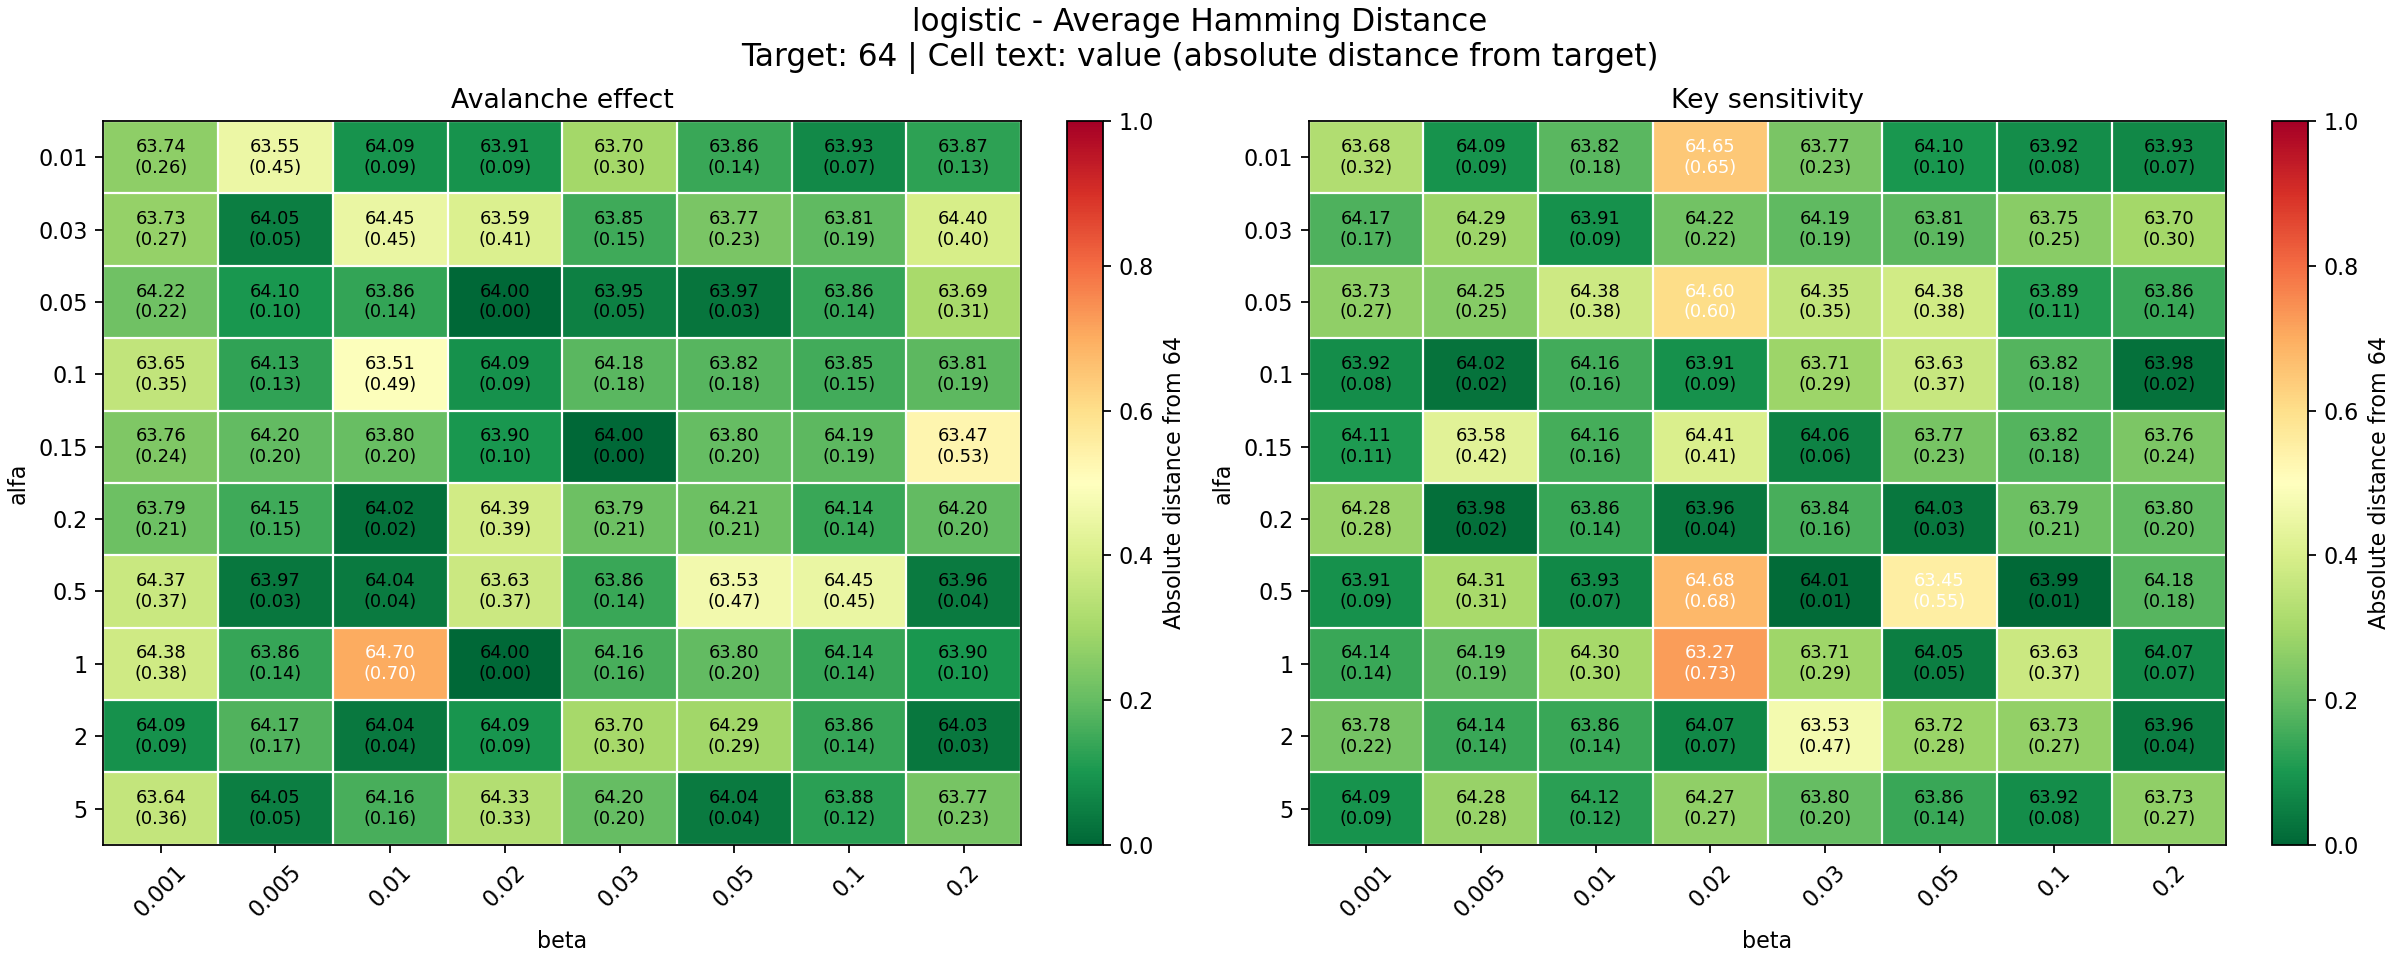
\includegraphics[width=1\textwidth]{images/logistic_hamming.png}
    \caption{Logistic map tests results on the first phase}
    \label{fig:logisticParams}
\end{figure}

\subsection{Stability Penalty System and Final Ranking}
To categorically avoid the selection of mathematically dangerous configurations that could degrade the cipher in edge cases, a penalty system was introduced. 
The penalty evaluates the system's structural integrity over the initial stability iterations, computing a weighted score based on three specific failure modes:
\begin{equation}
    P_{\text{stability}} = 100 \cdot R_{\text{saturation}} + 100 \cdot R_{\text{unstable}} + 1000 \cdot R_{\text{non-finite}}
\end{equation}
Where the penalty ratios ($R$) represent the number of failing samples over the total observed samples:
\begin{itemize}
    \item \textbf{Saturation Ratio ($R_{\text{saturation}}$):} Weighted at 100, this metric penalizes cases where the chaotic output is clamped to the asymptotic limits of the $\tanh$ function, thereby losing its dynamic behavior.
    
    \item \textbf{Instability Ratio ($R_{\text{unstable}}$):} Also weighted at 100, it reports algorithmic anomalies, such as the chaotic orbit unnaturally converging to a fixed structural limit.
    
    \item \textbf{Collapse Ratio ($R_{\text{non-finite}}$):} Heavily weighted at 1000, this is the most critical penalty. It targets combinations that cause the chaotic state to mathematically explode, resulting in \texttt{NaN} or \texttt{Infinity} values which would cause a catastrophic failure in an embedded CPU.
\end{itemize}

The final sorting metric (\texttt{total\_score}) is calculated by summing the absolute deviation ($dev_{\text{sum}}$) and the stability penalty ($P_{\text{stability}}$). 
The parameter pairs are ranked in strictly ascending order, prioritizing the lowest total score. 
In the event of a tie, the algorithm first prefers the pair with the lowest $dev_{\text{sum}}$. 
As a final tie-breaker, the framework selects the pair minimizing the maximum individual deviation, evaluated as $\max(dev_{\text{ks}}, dev_{\text{ae}})$, ensuring the highest worst-case performance guarantee for the chosen chaotic map.

\subsection{Selection Results and Parameter Assignment}
Following the rigorous Phase 2 confirmation iterations and the application of the mathematical stability penalties, the system isolated a single definitive set of parameters for each chaotic map. 
The final selected triads ($\alpha$, $\beta$, $\delta$) are detailed in Table~\ref{tab:chaotic_params_ranking}.

\begin{table}[htbp]
    \centering
    \small
    \setlength{\tabcolsep}{5.5pt}
    \begin{tabular}{lccccccc}
        \toprule
        \textbf{Map} & $\boldsymbol{\alpha}$ & $\boldsymbol{\beta}$ & $\boldsymbol{\delta}$ & $\overline{\textbf{HD}}_{\textbf{ks}}$ & $\textbf{Dev}_{\textbf{ks}}$ & $\overline{\textbf{HD}}_{\textbf{ae}}$ & $\textbf{Dev}_{\textbf{ae}}$ \\
        \midrule
        Logistic     & 0.50 & 0.010 &   0.0299 & 64.0413 & 0.0413 & 63.9720 & 0.0280 \\
        Tent         & 0.01 & 0.001 & 175.7223 & 64.0737 & 0.0737 & 64.1071 & 0.1071 \\
        Sine         & 0.03 & 0.001 &  60.3030 & 63.9724 & 0.0276 & 63.9224 & 0.0776 \\
        Chebyshev    & 0.03 & 0.001 &  28.4113 & 63.9660 & 0.0340 & 64.0588 & 0.0588 \\
        H\'enon      & 0.50 & 0.010 &   0.0216 & 64.0671 & 0.0671 & 63.9941 & 0.0059 \\
        Arnold       & 0.05 & 0.001 &  35.7719 & 63.9375 & 0.0625 & 64.0744 & 0.0744 \\
        Lorenz       & 0.03 & 0.010 &   2.1379 & 63.8746 & 0.1254 & 64.0437 & 0.0437 \\
        Chen         & 0.01 & 0.005 &  17.1727 & 64.1033 & 0.1033 & 63.9121 & 0.0879 \\
        R\"ossler    & 0.15 & 0.030 &   1.0235 & 63.9765 & 0.0235 & 63.9887 & 0.0113 \\
        \bottomrule
    \end{tabular}
    \caption{Optimal parameters ($\alpha$, $\beta$, $\delta$) and corresponding Key Sensitivity ($\text{HD}_{\text{ks}}$) and Avalanche Effect ($\text{HD}_{\text{ae}}$) Hamming Distances with their respective absolute deviations from the ideal 64-bit value.}
    \label{tab:chaotic_params_ranking}
\end{table}

As highlighted by the empirical data in Table~\ref{tab:chaotic_params_ranking}, every chaotic system, when initialized with its optimized parameter set, achieved statistically near-ideal cryptographic diffusion. 
The absolute deviations from the perfect 64-bit target strictly remained below a fraction of a single bit (maximum deviation $\approx 0.12$) across all tested architectures. 

This evidence definitively proves that integrating a scalar chaotic injection into the substitution routine does not degrade the strict bijectivity and fundamental security properties of the standardized AES cipher. 
Consequently, these specific optimized values have been hardcoded into the C implementation, acting as the default operational constants for all subsequent performance benchmarks and Side-Channel security evaluations.


\section{Randomness Properties Preservation}
Following the derivation of the optimal chaotic parameters, the subsequent validation phase entails the application of the official NIST Statistical Test Suite (SP 800-22 Rev 1a)~\cite{NISTRandomnessTestSuite}. 
This standard framework comprises 15 distinct statistical tests (effectively 16, as the Cumulative Sums test is evaluated across two modes) specifically designed to assess the randomness of pseudo-random number generators. 

In modern cryptographic literature, this suite is also rigorously employed to verify that the ciphertexts produced by symmetric encryption algorithms remain statistically indistinguishable from pure, unpredictable noise. 
Consequently, this study utilizes the NIST suite to formally prove that the chaotic modifications injected into the AES implementation preserve the pristine random properties characteristic of the unaltered baseline algorithm.

For the practical execution of the statistical analysis, this study integrates an open-source Python implementation of the NIST suite~\cite{stevenang2020randomness_testsuite}. 
To feed the analysis, exactly 1,000,000 bits (125,000 bytes) of ciphertext are generated for each map, evaluating them against the entire battery of tests.

\subsection{Evaluation Schemes and Metrics}
To interpret the results returned by each of the statistical tests, specific evaluation schemes are employed strictly adhering to the official NIST methodology~\cite{NISTRandomnessTestSuite}, 
which bases its validation upon \texttt{P-value} significance states. 

A \texttt{P-value} is a continuous variable within the interval $[0, 1]$. 
To successfully pass an individual statistical test, the returned \texttt{P-value} must be greater than or equal to the significance level $\alpha = 0.01$. 
By defining this threshold, the NIST standard explicitly acknowledges the probabilistic nature of the evaluation, accepting a 1\% mathematical probability that an inherently random sequence might be incorrectly flagged as a failure (Type I error).

Crucially, the overall validation of a cryptographic system cannot depend on a single evaluated sequence. 
Instead, an entire set of independently generated sequences must be analyzed to produce a statistically significant distribution capable of absorbing the 1\% error threshold. 
For the purpose of this study, the evaluation metric is established over a sequence count of 100 iterations for each chaotic map.

To prevent the application of an overly rigid ``one-out, all-out'' policy, where a single sequence failure would inexplicably compromise the entire cipher,
the assessment relies on the NIST proportion margin formula:
\begin{equation}
    \text{Margin} = 3 \cdot \sqrt{\frac{\text{Target}_{\text{prop}} \cdot (1 - \text{Target}_{\text{prop}})}{\text{Sequence}_{\text{count}}}}
\end{equation}
where $\text{Target}_{\text{prop}} = 1 - \alpha = 0.99$ and $\text{Sequence}_{\text{count}}$ is statically set to $100$. Evaluating the equation yields the absolute acceptance boundaries:
\begin{align*}
    \text{Lower Bound} &= 0.99 - 0.029849 \approx 0.9601 \\
    \text{Upper Bound} &= 0.99 + 0.029849 \approx 1.0198 \quad (\text{capped at } 1.0)
\end{align*}
Therefore, an individual NIST test is considered globally successful for a specific chaotic map only if at least 96\% of the 100 generated sequences yield a \texttt{P-value} $\ge 0.01$.

\paragraph{P-value Uniformity Analysis (Chi-Squared Test)}
Beyond achieving the minimum passing proportion, official NIST guidelines mandate that an optimal cryptosystem must produce a statistically uniform distribution of \texttt{P-values} across all tested sequences. 

To formally verify this uniformity, a $\chi^2$ (Chi-Squared) goodness-of-fit test is executed over the results. 
The 100 obtained \texttt{P-values} are partitioned into 10 equally spaced sub-intervals between 0 and 1. 
The empirical frequency of values falling into each bucket is then statistically compared against the ideal expected distribution ($E_i = \frac{\text{Sequence}_{\text{count}}}{10}$). 
Ultimately, an incomplete gamma function evaluates the $\chi^2$ statistic to calculate a final $P\text{-value}_{\text{uniformity}}$. 
The uniformity test is strictly considered successful only if this resultant value is greater than or equal to the secondary threshold of $\alpha_{\text{uniformity}} = 0.0001$.

\subsection{Statistical Results and Randomness Validation}
Following the execution of the complete NIST Statistical Test Suite, consisting of 100 iterations for each map, the empirical results confirm the robust cryptographic integrity of the chaotic architectures. 
To provide a comprehensive overview of the cipher's performance across the entire testing spectrum, Figure~\ref{fig:NIST_heatmap} presents a heatmap detailing the overall success trends.

\begin{figure}[htbp]
    \centering
    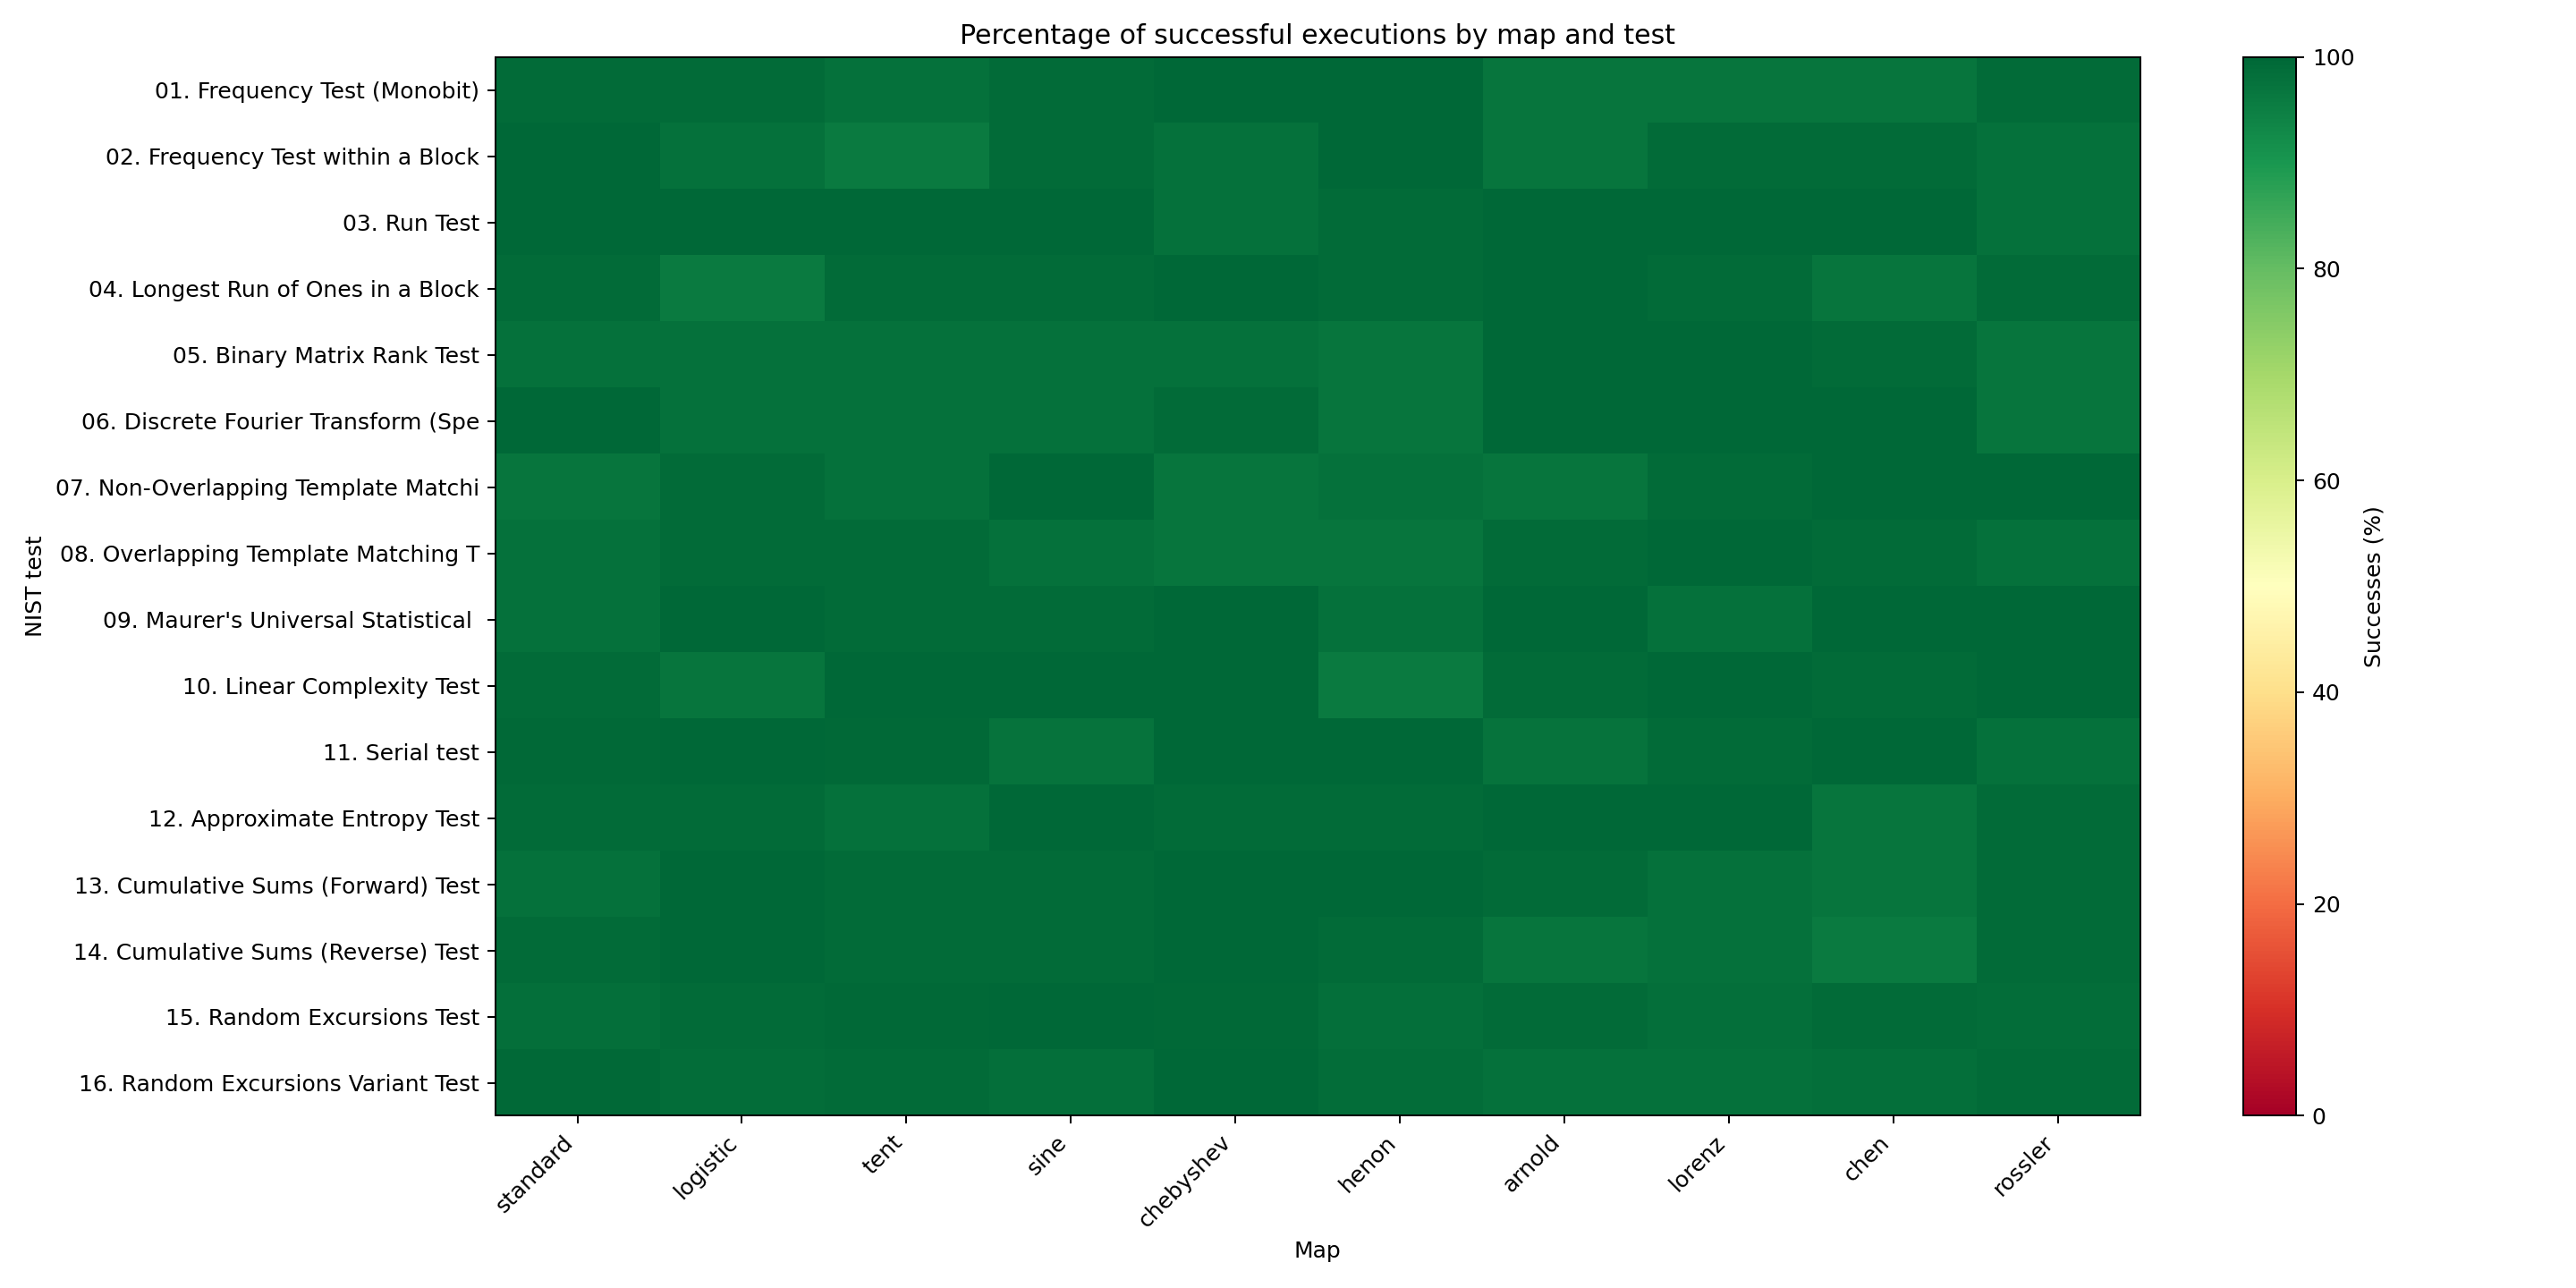
\includegraphics[width=1.1\textwidth]{images/success_rate_heatmap.png}
    \caption{Heatmap illustrating the percentage of successful sequences for each NIST statistical test across the baseline AES and the chaotic map variants.}
    \label{fig:NIST_heatmap}
\end{figure}

As highlighted by the average success rate comparison in Figure~\ref{fig:NIST_results}, the chaotic systems maintain exceptionally high randomness properties. 
Notably, the Chebyshev map stands out, achieving an average success rate of 99.44\%, slightly surpassing the 98.97\% baseline of the standard AES. 
Conversely, the remaining chaotic maps exhibit marginally lower scores compared to the default cipher, with the Arnold Cat map recording the lowest average at 98.43\%. 
However, it is crucial to emphasize that all implementations drastically exceed the mathematically required lower bound of 96.01\%, solidifying the overall chaotic alteration as a definitive success.

\begin{figure}[H]
    \centering
    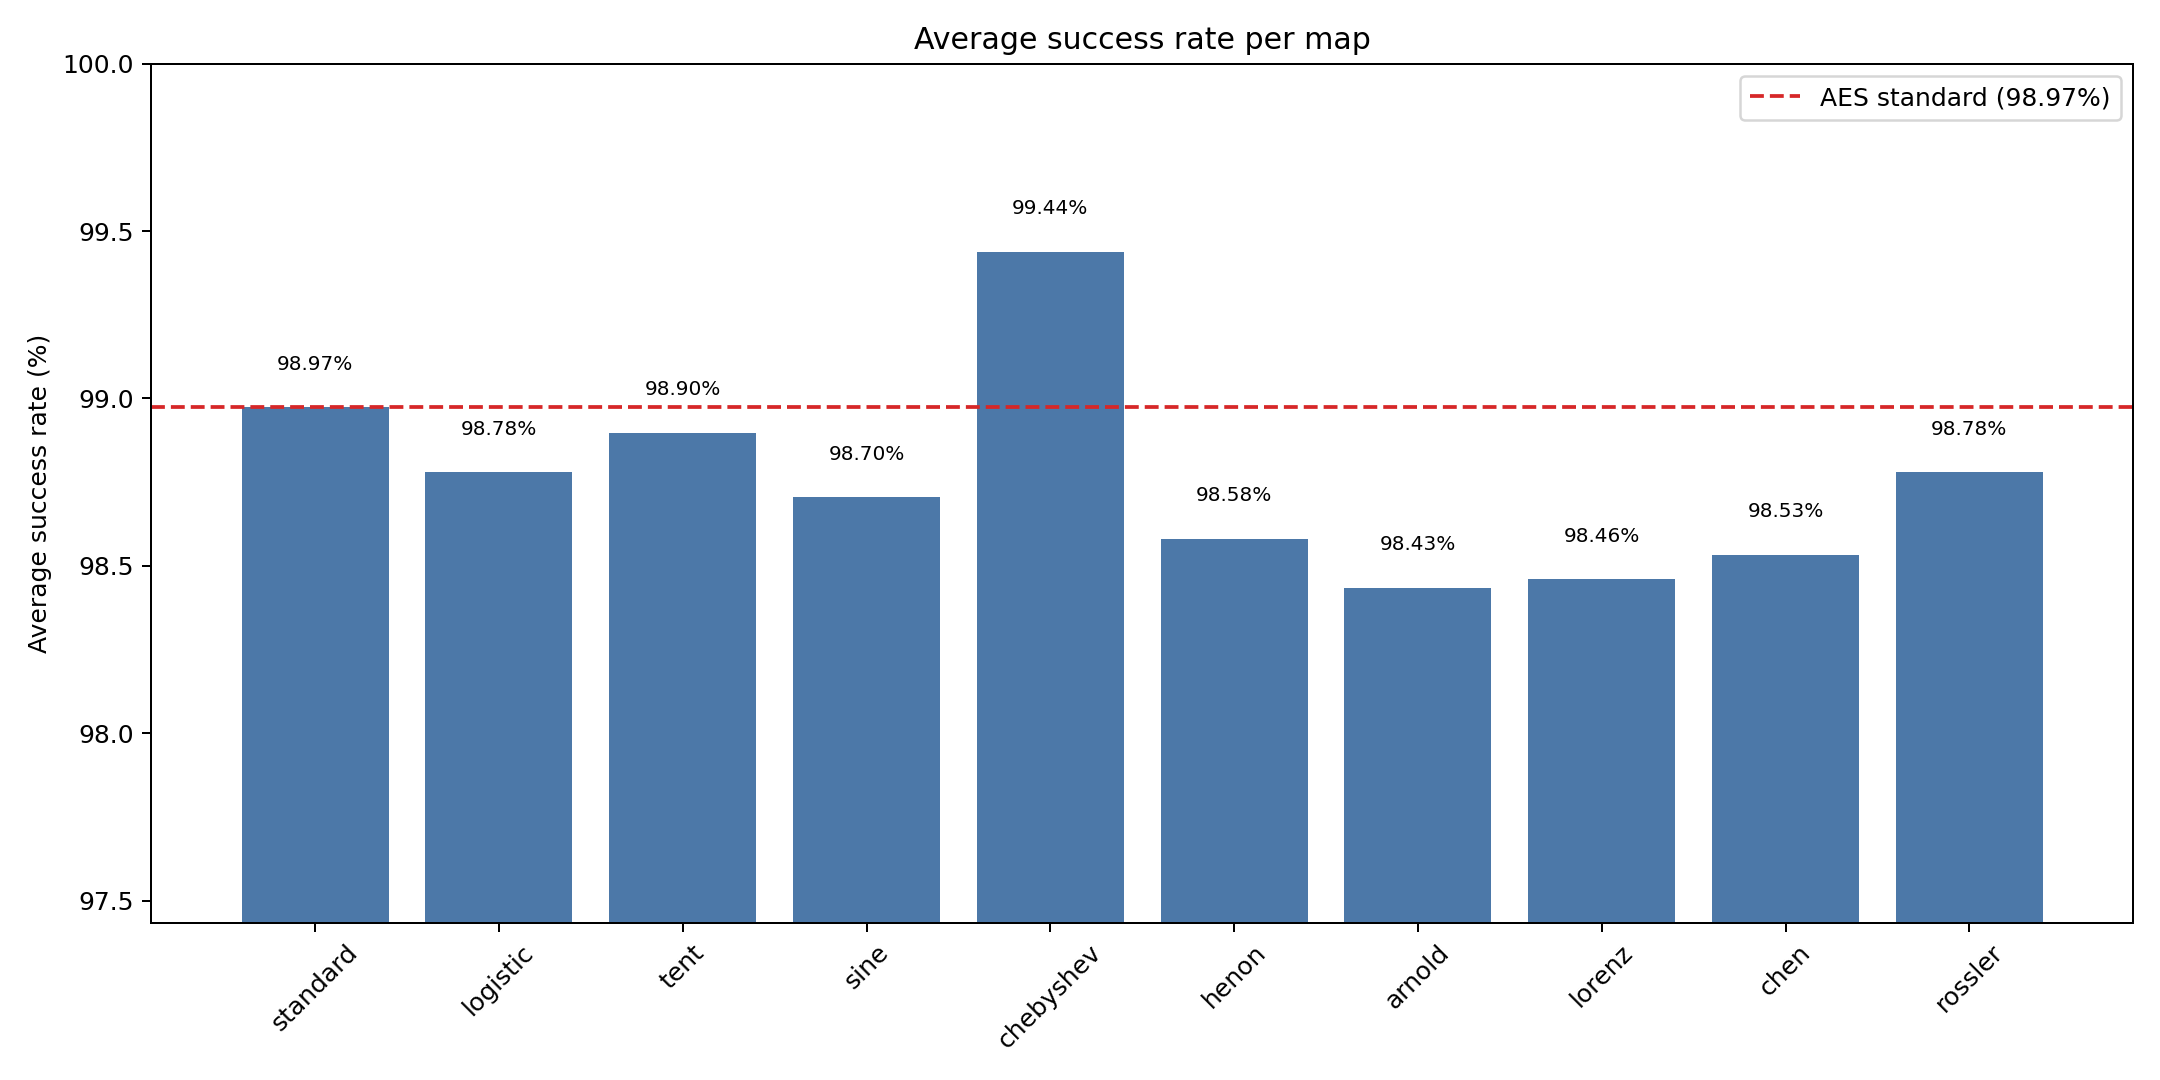
\includegraphics[width=0.9\textwidth]{images/average_success_rate.png}
    \caption{Average NIST success rate comparison between the standard AES implementation and the chaotic variants.}
    \label{fig:NIST_results}
\end{figure}

Continuing with the P-value uniformity analysis, Figure~\ref{fig:NIST_p-val} illustrates a highly satisfactory distribution for each chaotic map. 
While minor local frequency variations are visually observable, such as a slightly more fluctuating distribution in the Chen and Hénon systems, alongside a noticeable initial frequency spike in the Lorenz system, these variations remain well within statistical tolerances. 
The dedicated $\chi^2$ uniformity evaluation confirmed a 100\% pass rate across all implementations, formally validating that the P-values are sufficiently and evenly distributed.

Finally, the vertical red dashed line in Figure~\ref{fig:NIST_p-val} represents the $\alpha = 0.01$ rejection threshold. 
The histograms clearly demonstrate that only a mathematically expected, minor subset of tests fell below this limit for each chaotic system, identically mirroring the behavior of the standard AES. 
This provides a textbook empirical observation of the Type I error (false positive) rate formally acknowledged by the NIST standard.

\begin{figure}[htbp]
    \centering
    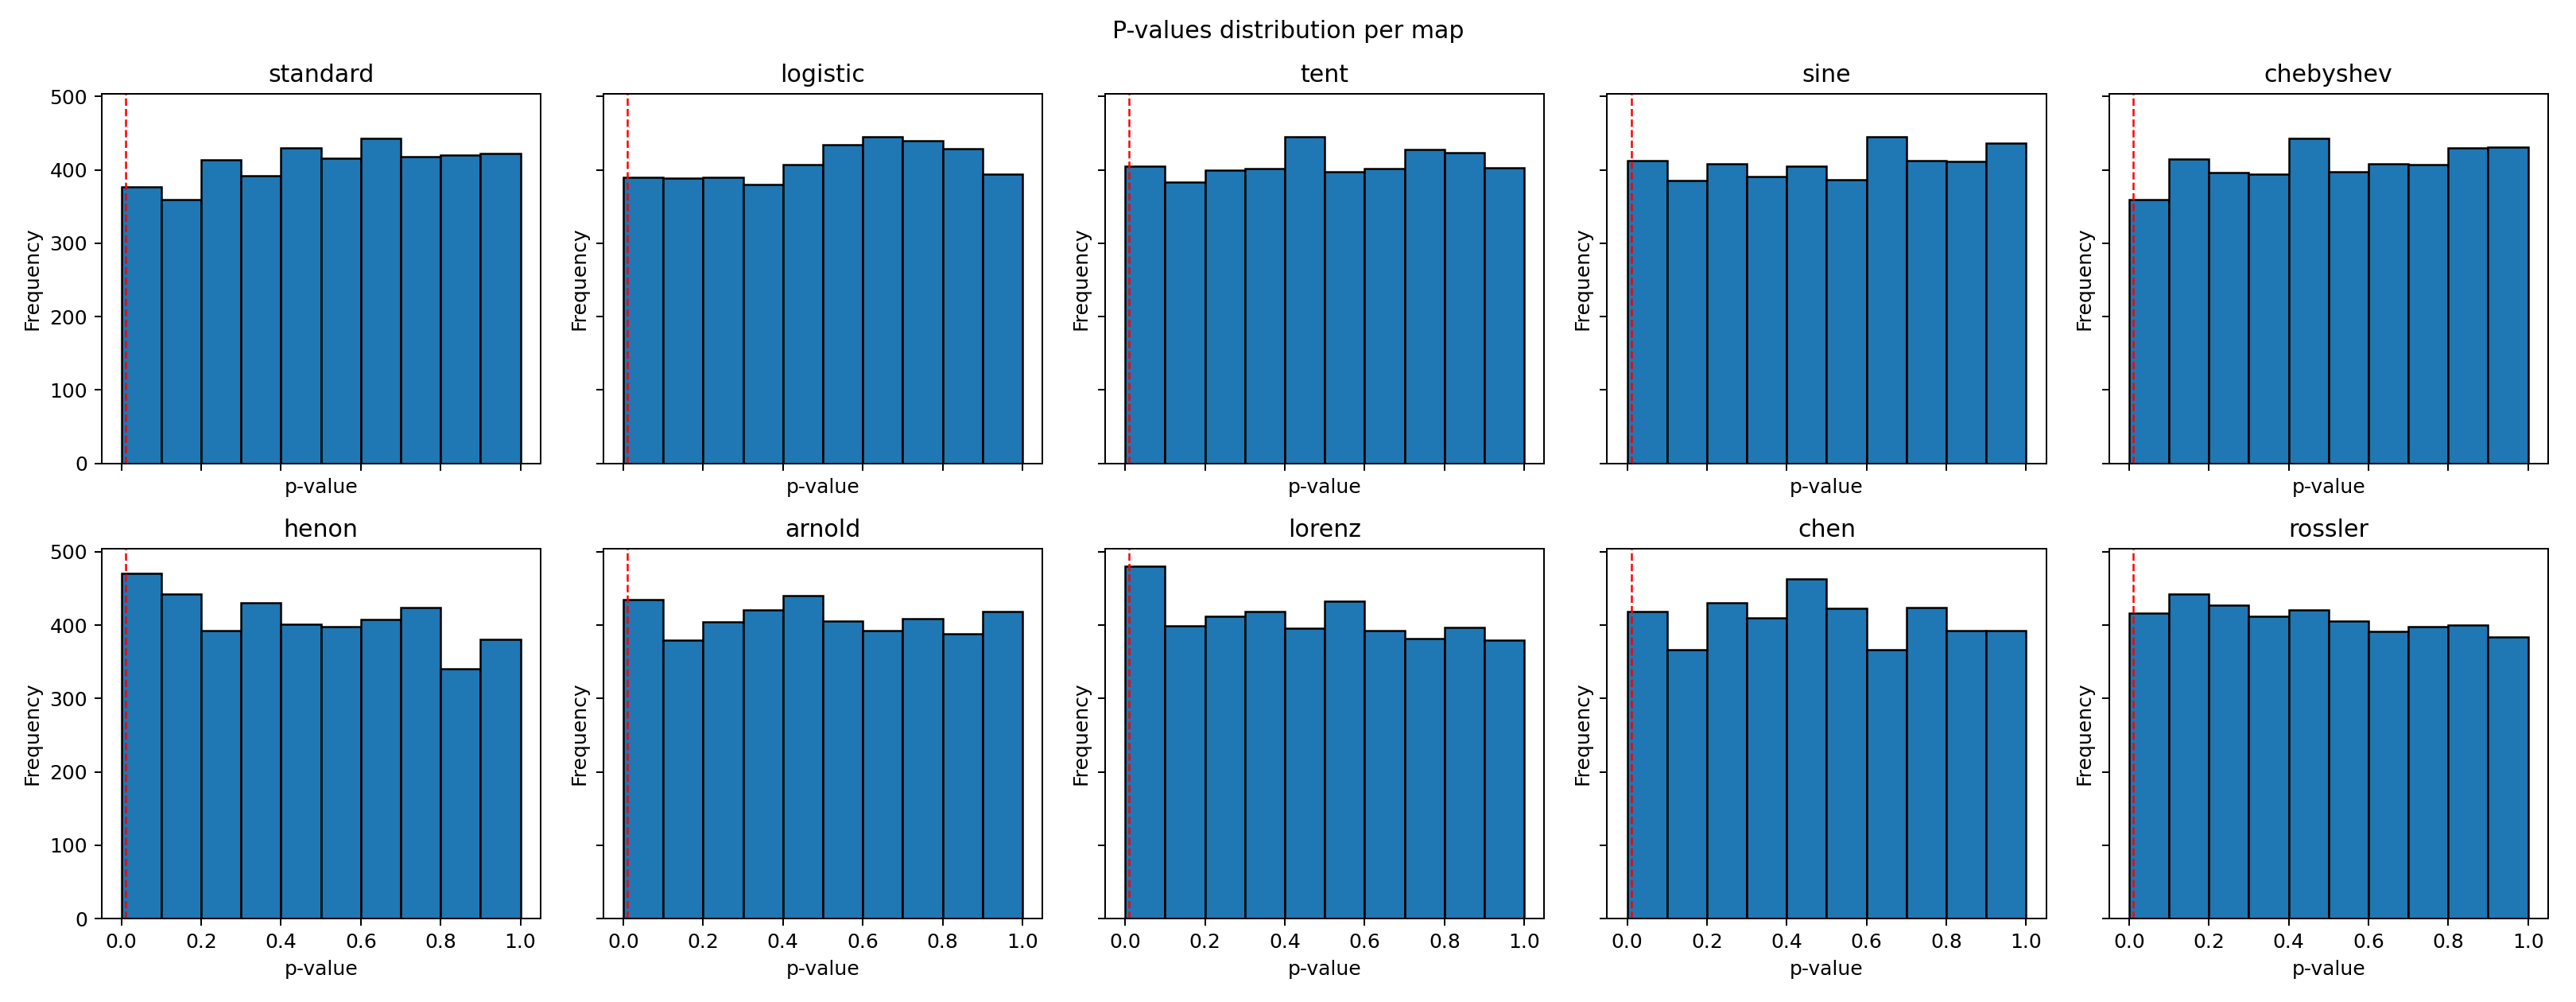
\includegraphics[width=1\textwidth]{images/p_value_distributions.png}
    \caption{Frequency distributions of P-values for each cryptographic configuration, visually confirming the required statistical uniformity.}
    \label{fig:NIST_p-val}
\end{figure}

\section{Benchmark and SWaP analysis}
Before evaluating the physical performance metrics of the embedded implementation, a brief theoretical premise regarding the cipher's mathematical cryptanalysis resistance is required. 
In the foundational study by Kumar et al.~\cite{KumarPaper}, the authors benchmarked chaotic S-Boxes against linear and differential cryptanalysis using the Logistic and Hénon maps as their primary case studies. 

As reported in their theoretical analysis, dynamically perturbing the S-Box introduces a marginal mathematical trade-off: individual chaotic maps cause a slight fluctuation in the \textit{Non-Linearity (NL)} score (dipping from the standard 112 to approximately 108-110) and a minor increase in \textit{Differential Uniformity (DU)} (from the baseline 4.0 to 5.0-6.0). 
In cryptographic engineering, this represents a well-documented and acceptable compromise: a minimal reduction of theoretical algebraic bounds in exchange for a massive increase in micro-architectural side-channel resilience. 

Because the scalar optimization proposed in this thesis applies the exact same bounded mathematical perturbation (via the $\gamma \cdot \tanh$ limiter) across all evaluated maps, these marginal DU and NL fluctuations are inherently inherited. 
Furthermore, the near-perfect Avalanche Effect and strict NIST randomness scores obtained in the previous sections provide robust empirical confirmation that the cipher's structural integrity remains highly secure. 

Consequently, rather than replicating the theoretical algebraic cryptanalysis already validated by the reference literature, the focal point of this evaluation shifts entirely to the physical and architectural viability of the cipher. 
The primary objective of the following benchmarks is to quantitatively analyze the computational trade-offs, specifically execution time, data throughput, and relative energy consumption, between the baseline AES-256-GCM, the theoretical \texttt{once-per-round} chaotic update, 
and the highly optimized \texttt{once-per-block} strategy introduced in this study.

Such performance analysis is essential for delicate contexts such as SATCOM, which are subject to strict \texttt{SWaP} (Size, Weight, and Power) constraints due to the adverse environments in which they operate.

The empirical measurements for this study were executed on a university computing cluster, utilizing an AMD EPYC 7301 16-Core Processor (x86\_64). 
The node features a dual-socket architecture (32 physical cores total), of which 8 cores were strictly allocated for the concurrent measurements running on Ubuntu 24.04.2 LTS. 

The objective of these benchmarks is not to record the absolute maximum speed achievable on enterprise hardware, but rather to extract the relative performance delta (i.e. the overhead)
between the baseline AES implementation and the chaotic injected variants.

For both the \texttt{once-per-round} and \texttt{once-per-block} chaos-update implementations, 
the measurements are based on 1,000 iterations over a fixed-size payload of 5~MB.

\subsection{Once-per-Round Update Benchmarks}
As detailed in Table~\ref{tab:table_opr}, the \texttt{once-per-round} chaotic update strategy introduces an expected, quantifiable increase in the total execution time for both the encryption and decryption phases, with a consequent reduction in data throughput. 
The magnitude of this overhead scales directly with the mathematical complexity of the chosen chaotic map.

\begin{table}[htbp]
    \centering
    \footnotesize
    \setlength{\tabcolsep}{6pt}
    \resizebox{\textwidth}{!}{%
    \begin{tabular}{llcccccc}
        \toprule
        \textbf{Map} & \textbf{Phase} & \textbf{Total Time (s)} & \textbf{Avg. Time (s)} & \textbf{Std. Dev. (s)} & \textbf{Throughput (MB/s)} & \textbf{Time Overhead} & \textbf{Throughput Overhead} \\
        \midrule
        AES-GCM standard         & Encryption & 1680.54 & 1.68 & 0.01 & 2.98 &   0.00\% &   0.00\% \\
        AES-GCM standard         & Decryption & 1659.08 & 1.66 & 0.02 & 3.01 &   0.00\% &   0.00\% \\ \midrule
        AES-GCM Logistic Map     & Encryption & 1754.95 & 1.75 & 0.01 & 2.85 &  +4.43\% &  -4.24\% \\
        AES-GCM Logistic Map     & Decryption & 1742.39 & 1.74 & 0.01 & 2.87 &  +5.02\% &  -4.78\% \\ \midrule
        AES-GCM Tent Map         & Encryption & 1770.57 & 1.77 & 0.01 & 2.82 &  +5.36\% &  -5.08\% \\
        AES-GCM Tent Map         & Decryption & 1755.87 & 1.76 & 0.02 & 2.85 &  +5.83\% &  -5.51\% \\ \midrule
        AES-GCM Sine Map         & Encryption & 1866.97 & 1.87 & 0.01 & 2.68 & +11.09\% &  -9.99\% \\
        AES-GCM Sine Map         & Decryption & 1883.58 & 1.88 & 0.01 & 2.65 & +13.53\% & -11.92\% \\ \midrule
        AES-GCM Chebyshev Map    & Encryption & 2023.80 & 2.02 & 0.01 & 2.47 & +20.43\% & -16.96\% \\
        AES-GCM Chebyshev Map    & Decryption & 2042.37 & 2.04 & 0.00 & 2.45 & +23.10\% & -18.77\% \\ \midrule
        AES-GCM H\'enon Map      & Encryption & 1754.79 & 1.75 & 0.01 & 2.85 &  +4.42\% &  -4.23\% \\
        AES-GCM H\'enon Map      & Decryption & 1771.92 & 1.77 & 0.00 & 2.82 &  +6.80\% &  -6.37\% \\ \midrule
        AES-GCM Arnold Cat Map   & Encryption & 1822.31 & 1.82 & 0.01 & 2.74 &  +8.44\% &  -7.78\% \\
        AES-GCM Arnold Cat Map   & Decryption & 1810.85 & 1.81 & 0.01 & 2.76 &  +9.15\% &  -8.38\% \\ \midrule
        AES-GCM Lorenz Map       & Encryption & 2078.60 & 2.08 & 0.02 & 2.41 & +23.69\% & -19.15\% \\
        AES-GCM Lorenz Map       & Decryption & 2101.50 & 2.10 & 0.00 & 2.38 & +26.67\% & -21.05\% \\ \midrule
        AES-GCM Chen Map         & Encryption & 2081.55 & 2.08 & 0.01 & 2.40 & +23.86\% & -19.26\% \\
        AES-GCM Chen Map         & Decryption & 2067.99 & 2.07 & 0.02 & 2.42 & +24.65\% & -19.77\% \\ \midrule
        AES-GCM R\"ossler Map    & Encryption & 2049.63 & 2.05 & 0.01 & 2.44 & +21.96\% & -18.01\% \\
        AES-GCM R\"ossler Map    & Decryption & 2059.12 & 2.06 & 0.00 & 2.43 & +24.11\% & -19.43\% \\
        \bottomrule
    \end{tabular}%
    }
    \caption{Execution time, throughput, and relative performance overhead across standard AES-256-GCM and chaotic map configurations during encryption and decryption in Once-per-round mode (1000 iterations, 5.0 MB payload).}
    \label{tab:table_opr}
\end{table}

Visually supported by Figure~\ref{fig:opr_time}, the empirical data reveals clear performance tiers based on the architectural dimensionality of the maps. 
The simpler one-dimensional systems (Logistic and Tent) prove highly efficient, maintaining a stable time overhead of only $\approx 4.5\%$ to $5.5\%$. 
The two-dimensional discrete maps (Hénon and Arnold Cat) exhibit a similar lightweight profile, with Hénon actually matching the Logistic map's performance ($+4.42\%$). 

Conversely, the Sine and Chebyshev equations introduce steeper penalties (up to $+23\%$), largely due to the heavy reliance on the host CPU's Floating-Point Unit (FPU) to compute complex trigonometric functions dynamically. 
Finally, as mathematically expected, the three-dimensional continuous ODE maps (Lorenz, Chen, Rössler) demand the highest execution overhead (up to $+26.67\%$), severely degrading the system's throughput.

\begin{figure}[htbp]
    \centering
    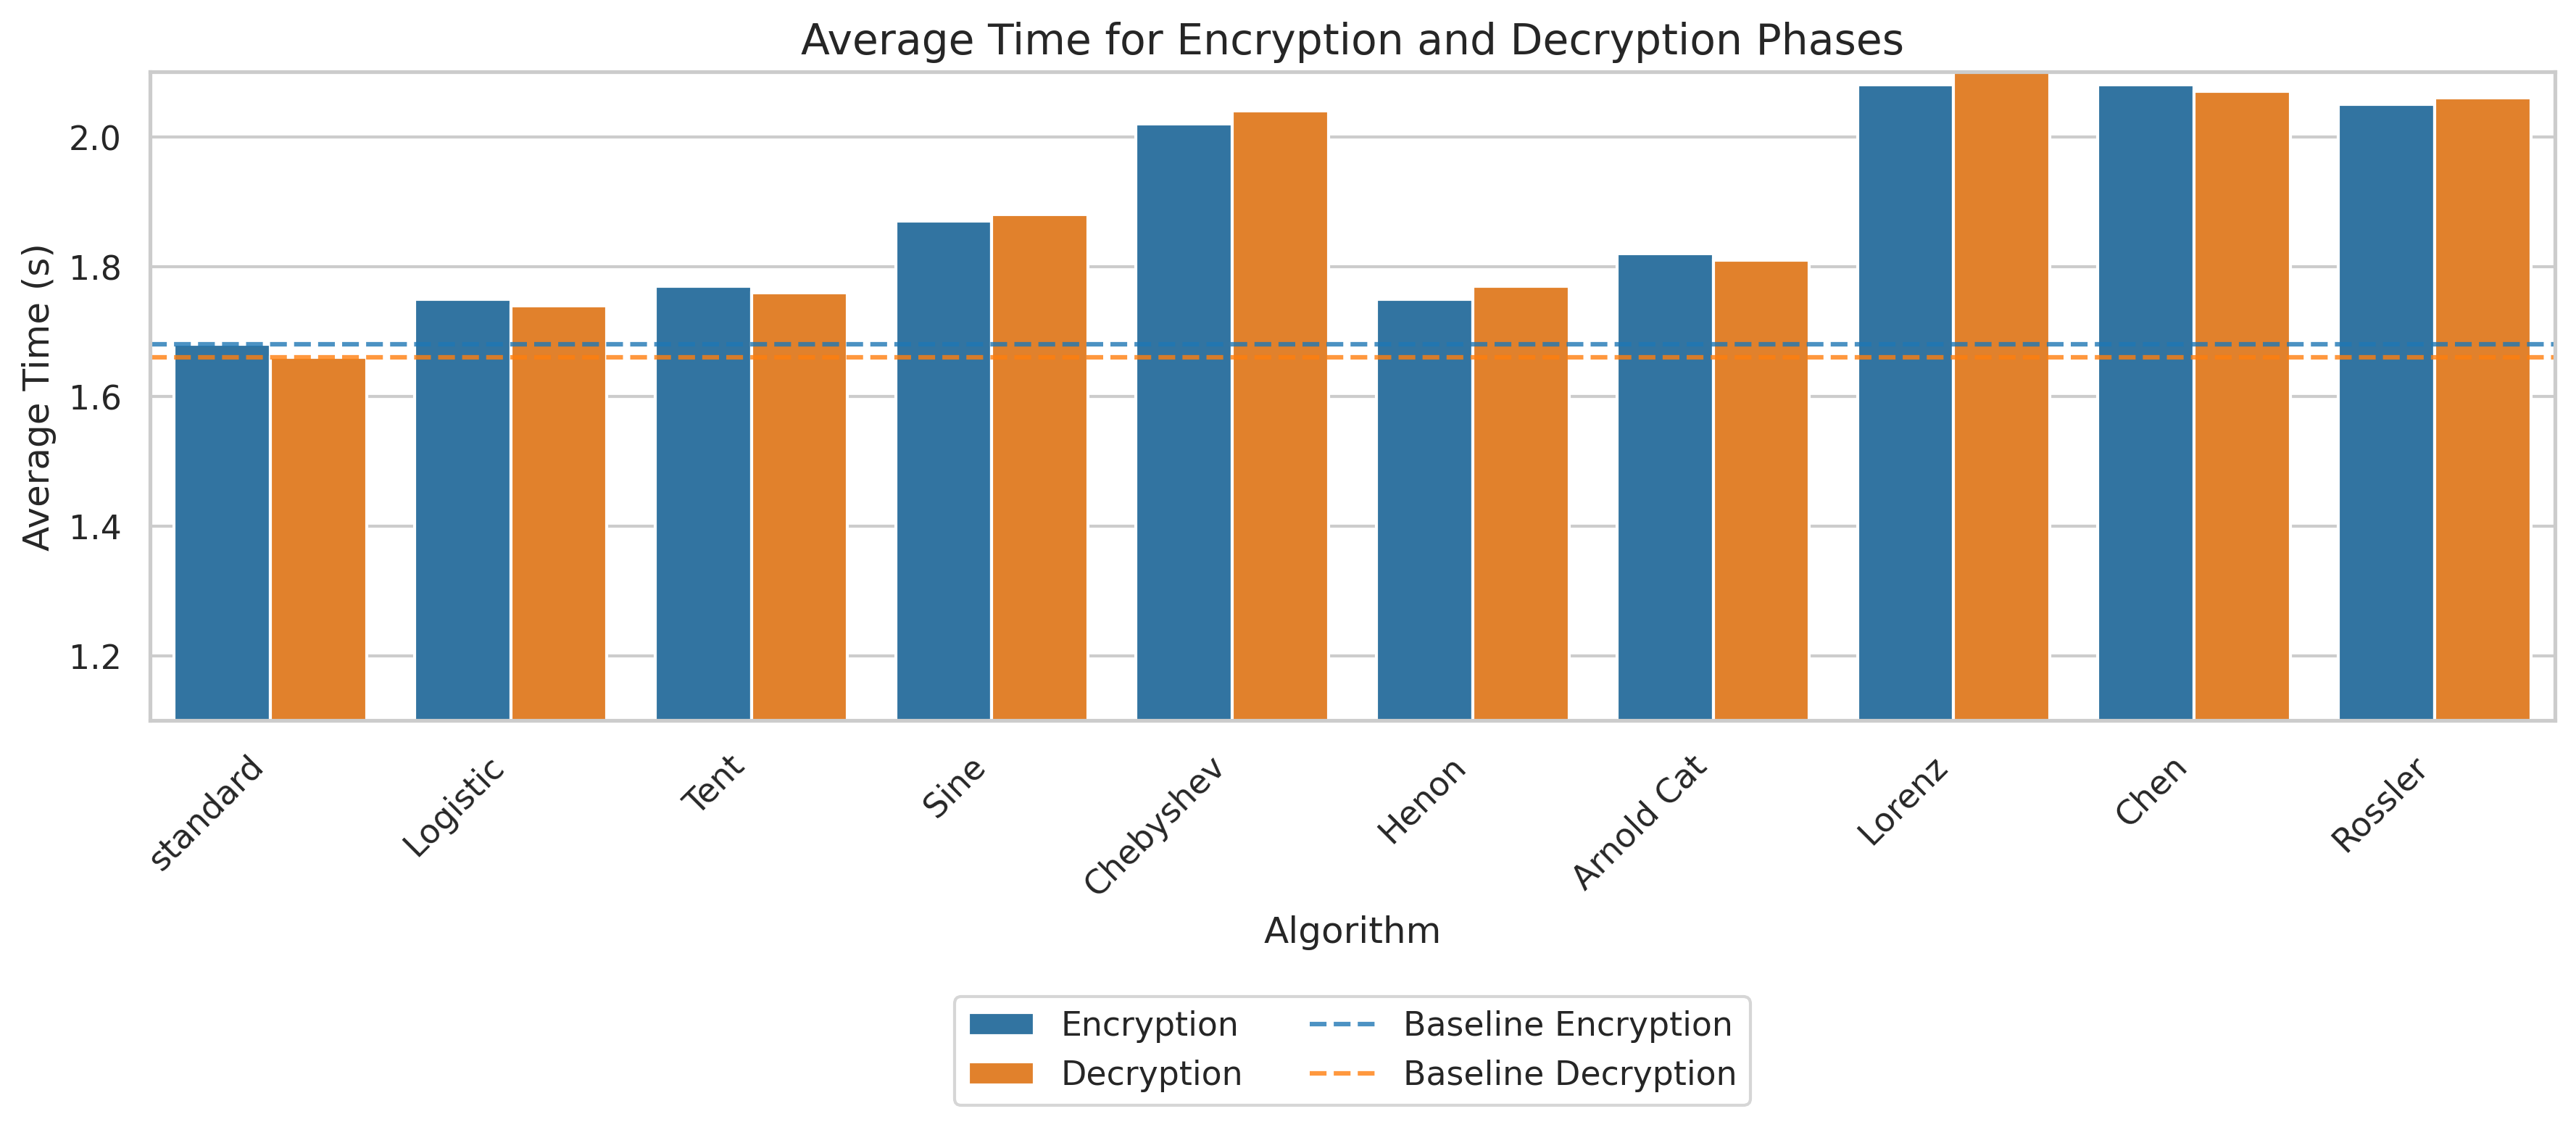
\includegraphics[width=0.9\textwidth]{images/Time_opr.png}
    \caption{Average execution time comparison for the \texttt{once-per-round} chaotic injection architecture against the standard AES baseline.}
    \label{fig:opr_time}
\end{figure}

\paragraph{Execution Time as an Energy Proxy}
Due to the restricted execution privileges on the shared cluster architecture, direct hardware telemetry (such as reading the CPU's RAPL registers to extract the exact Joule dissipation) was unavailable. 
However, in embedded engineering, execution time serves as a highly reliable linear proxy for energy consumption. 

Assuming that the active power draw ($P_{\text{active}}$) of the processor remains relatively constant while the single thread maximizes the core utilization to execute the cipher, 
the total energy consumed ($E = P_{\text{active}} \times t$) becomes directly proportional to the total execution time. 
Consequently, the time overhead percentages recorded in Table~\ref{tab:table_opr} translate strictly into energetic overheads. 
Implementing the \texttt{once-per-round} Rössler map, for example, would drain the satellite's battery $\approx 24\%$ faster than the standard AES algorithm. 
This significant energy penalty highlights the critical necessity of introducing the optimized \texttt{once-per-block} updating strategy.

\paragraph{Memory Footprint and SWaP Viability}
To complete the architectural profiling of the \texttt{once-per-\\round} implementation, it is imperative to analyze its memory footprint, a critical metric for devices subjected to strict SWaP constraints. 
Figure~\ref{fig:memory_footprint} illustrates the combined Stack and Heap memory usage for each configuration during execution.

\begin{figure}[htbp]
    \centering
    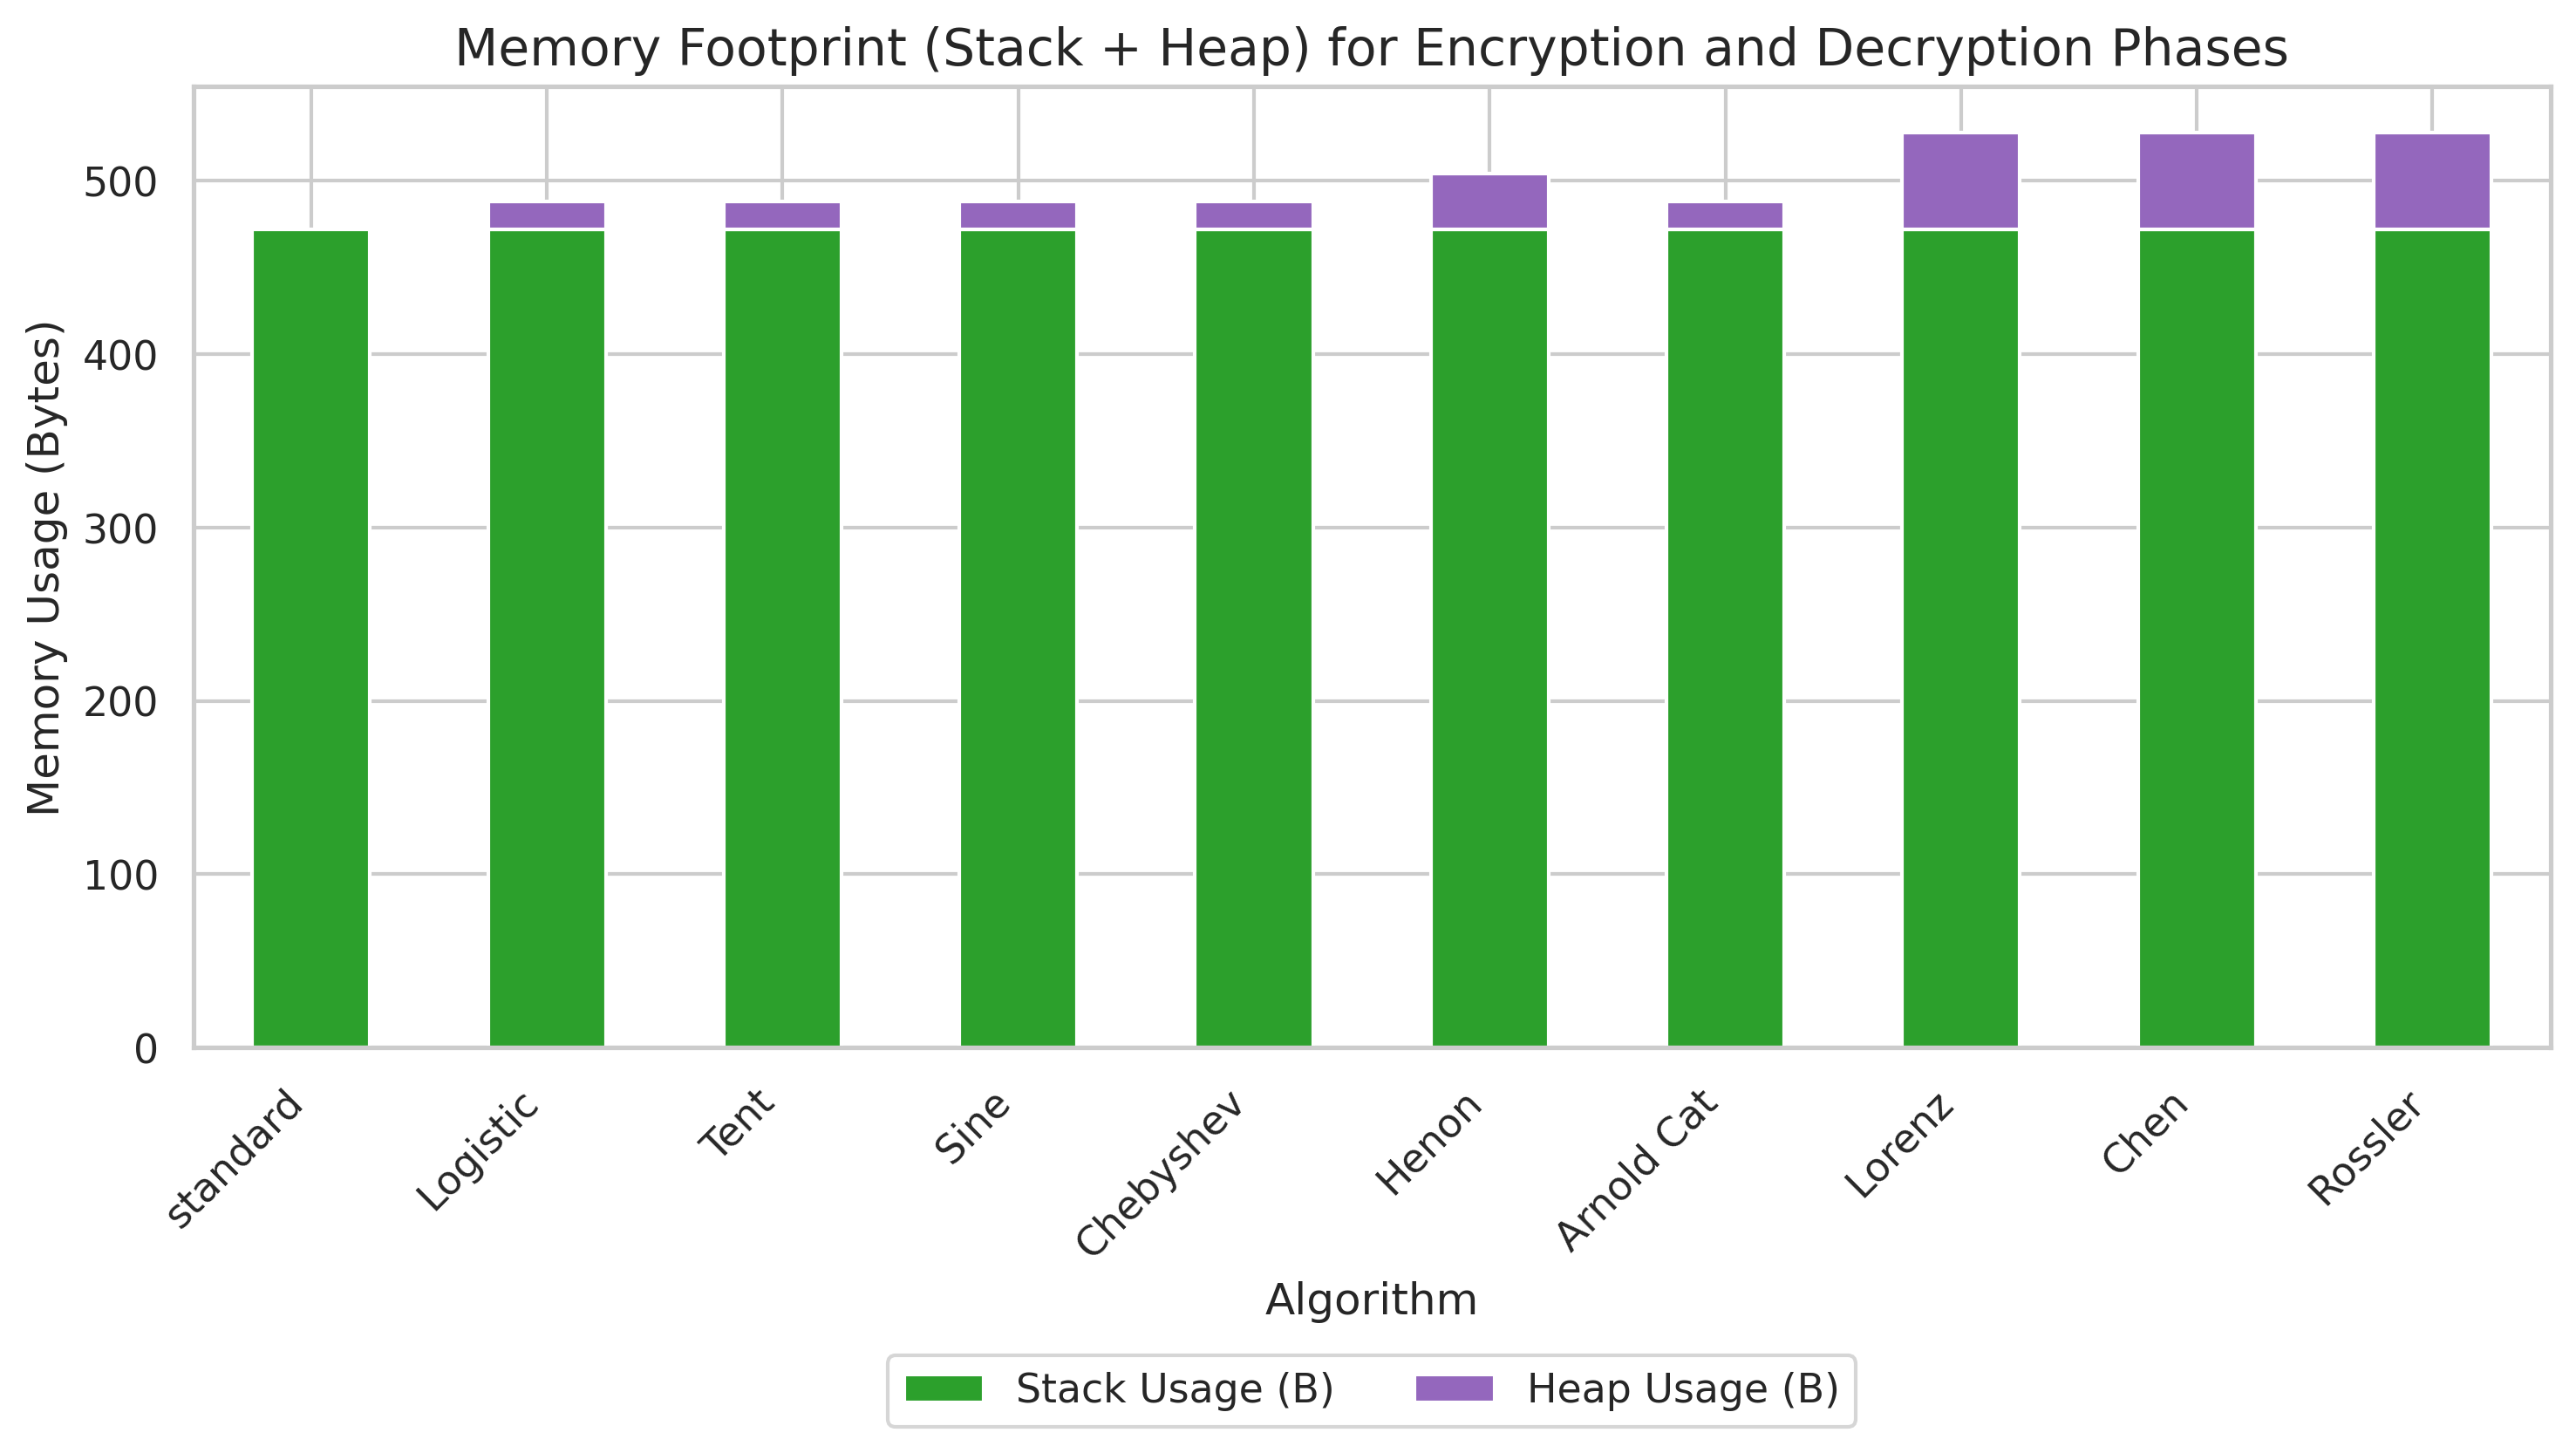
\includegraphics[width=\textwidth]{images/Memory_Footprint.png}
    \caption{Memory footprint analysis detailing Stack and Heap usage across the standard AES and chaotic configurations.}
    \label{fig:memory_footprint}
\end{figure}

The empirical measurements reveal a highly efficient memory utilization. 
The baseline AES implementation operates almost entirely within the Stack ($\approx 472$ Bytes). The introduction of the chaotic maps introduces a deterministic, mathematically proportional memory overhead allocated in the Heap. 
Specifically, one-dimensional maps (e.g., Logistic, Tent) require a mere 16 additional bytes to store their state parameters. 
This requirement logically scales to 32 bytes for the two-dimensional Hénon map, and peaks at exactly 56 extra bytes for the complex three-dimensional continuous systems (Lorenz, Chen, Rössler), which must continuously track multiple spatial coordinates.

It is important to contextualize that this dynamic Heap allocation is primarily an artifact of the modular testing environment, designed to swap chaotic parameters at runtime. 
In a production-grade firmware deployed on a satellite, these parameters would be statically compiled into the Stack or flash memory. 
Regardless of the allocation strategy, a maximum memory overhead of 56 Bytes is absolutely negligible even for the most constrained embedded microcontrollers, confirming that the chaotic injection satisfies the ``Size'' requirement of the aerospace SWaP paradigm flawlessly.

\subsection{Once-per-Block Update Benchmarks}
Finally, the exact same empirical benchmark suite was executed against the newly proposed \texttt{once-per-block} chaotic update strategy. 
The execution times and throughput measurements are detailed in Table~\ref{tab:table_opb}.

\begin{table}[htbp]
    \centering
    \footnotesize
    \setlength{\tabcolsep}{4.5pt}
    \resizebox{\textwidth}{!}{%
    \begin{tabular}{llcccccc}
        \toprule
        \textbf{Map} & \textbf{Phase} & \textbf{Total Time (s)} & \textbf{Avg. Time (s)} & \textbf{Std. Dev. (s)} & \textbf{Throughput (MB/s)} & \textbf{Time Overhead} & \textbf{Throughput Overhead} \\
        \midrule
        AES-GCM standard         & Encryption & 1656.78 & 1.66 & 0.01 & 3.02 &   0.00\% &   0.00\% \\
        AES-GCM standard         & Decryption & 1652.02 & 1.65 & 0.01 & 3.03 &   0.00\% &   0.00\% \\ \midrule
        AES-GCM Logistic Map     & Encryption & 1666.82 & 1.67 & 0.01 & 3.00 &  +0.61\% &  -0.60\% \\
        AES-GCM Logistic Map     & Decryption & 1675.54 & 1.68 & 0.01 & 2.98 &  +1.42\% &  -1.40\% \\ \midrule
        AES-GCM Tent Map         & Encryption & 1665.86 & 1.67 & 0.02 & 3.00 &  +0.55\% &  -0.54\% \\
        AES-GCM Tent Map         & Decryption & 1680.35 & 1.68 & 0.01 & 2.98 &  +1.71\% &  -1.69\% \\ \midrule
        AES-GCM Sine Map         & Encryption & 1686.06 & 1.69 & 0.00 & 2.97 &  +1.77\% &  -1.74\% \\
        AES-GCM Sine Map         & Decryption & 1685.73 & 1.69 & 0.01 & 2.97 &  +2.04\% &  -2.00\% \\ \midrule
        AES-GCM Chebyshev Map    & Encryption & 1691.12 & 1.69 & 0.02 & 2.96 &  +2.07\% &  -2.03\% \\
        AES-GCM Chebyshev Map    & Decryption & 1701.57 & 1.70 & 0.00 & 2.94 &  +3.00\% &  -2.91\% \\ \midrule
        AES-GCM H\'enon Map      & Encryption & 1674.95 & 1.67 & 0.00 & 2.99 &  +1.10\% &  -1.08\% \\
        AES-GCM H\'enon Map      & Decryption & 1670.29 & 1.67 & 0.03 & 2.99 &  +1.11\% &  -1.09\% \\ \midrule
        AES-GCM Arnold Cat Map   & Encryption & 1681.14 & 1.68 & 0.00 & 2.97 &  +1.47\% &  -1.45\% \\
        AES-GCM Arnold Cat Map   & Decryption & 1686.57 & 1.69 & 0.02 & 2.96 &  +2.09\% &  -2.05\% \\ \midrule
        AES-GCM Lorenz Map       & Encryption & 1703.94 & 1.70 & 0.01 & 2.93 &  +2.85\% &  -2.77\% \\
        AES-GCM Lorenz Map       & Decryption & 1718.94 & 1.72 & 0.01 & 2.91 &  +4.05\% &  -3.89\% \\ \midrule
        AES-GCM Chen Map         & Encryption & 1664.71 & 1.66 & 0.06 & 3.00 &  +0.48\% &  -0.48\% \\
        AES-GCM Chen Map         & Decryption & 1702.31 & 1.70 & 0.01 & 2.94 &  +3.04\% &  -2.95\% \\ \midrule
        AES-GCM R\"ossler Map    & Encryption & 1681.62 & 1.68 & 0.05 & 2.97 &  +1.50\% &  -1.48\% \\
        AES-GCM R\"ossler Map    & Decryption & 1704.87 & 1.70 & 0.00 & 2.93 &  +3.20\% &  -3.10\% \\
        \bottomrule
    \end{tabular}%
    }
    \caption{Execution time, throughput, and relative performance overhead across standard AES-256-GCM and chaotic map configurations during encryption and decryption in the \texttt{once-per-block} mode (1000 iterations, 5.0 MB payload).}
    \label{tab:table_opb}
\end{table}

By structurally reducing the frequency of chaotic state updates from 14 times per block (14 rounds in AES-256) down to a single instance, the entire set of implementations registers a drastic reduction in computational overhead. 
The one-dimensional baseline maps (Logistic and Tent) achieve near-zero performance degradation, peaking at a negligible $+0.61\%$ encryption time overhead. 
More importantly, the mathematically prohibitive trigonometric maps (Sine and Chebyshev) managed to heavily compress their maximum time augmentation down to $\approx 2\% - 3\%$, a radical improvement compared to the $+23\%$ penalty suffered in the previous configuration. 
Even the highly complex three-dimensional continuous ODEs (Lorenz, Chen, Rössler) effectively neutralized their CPU demand, falling within a maximum $+4\%$ time overhead boundary.

Figure~\ref{fig:opb_time} provides a visual representation of this performance optimization. 
By maintaining the same vertical axis limits as Figure~\ref{fig:opr_time}, the sheer scale of the computational gain becomes immediately apparent, with the chaotic implementations now performing almost indistinguishably from the AES baseline.

\begin{figure}[htbp]
    \centering
    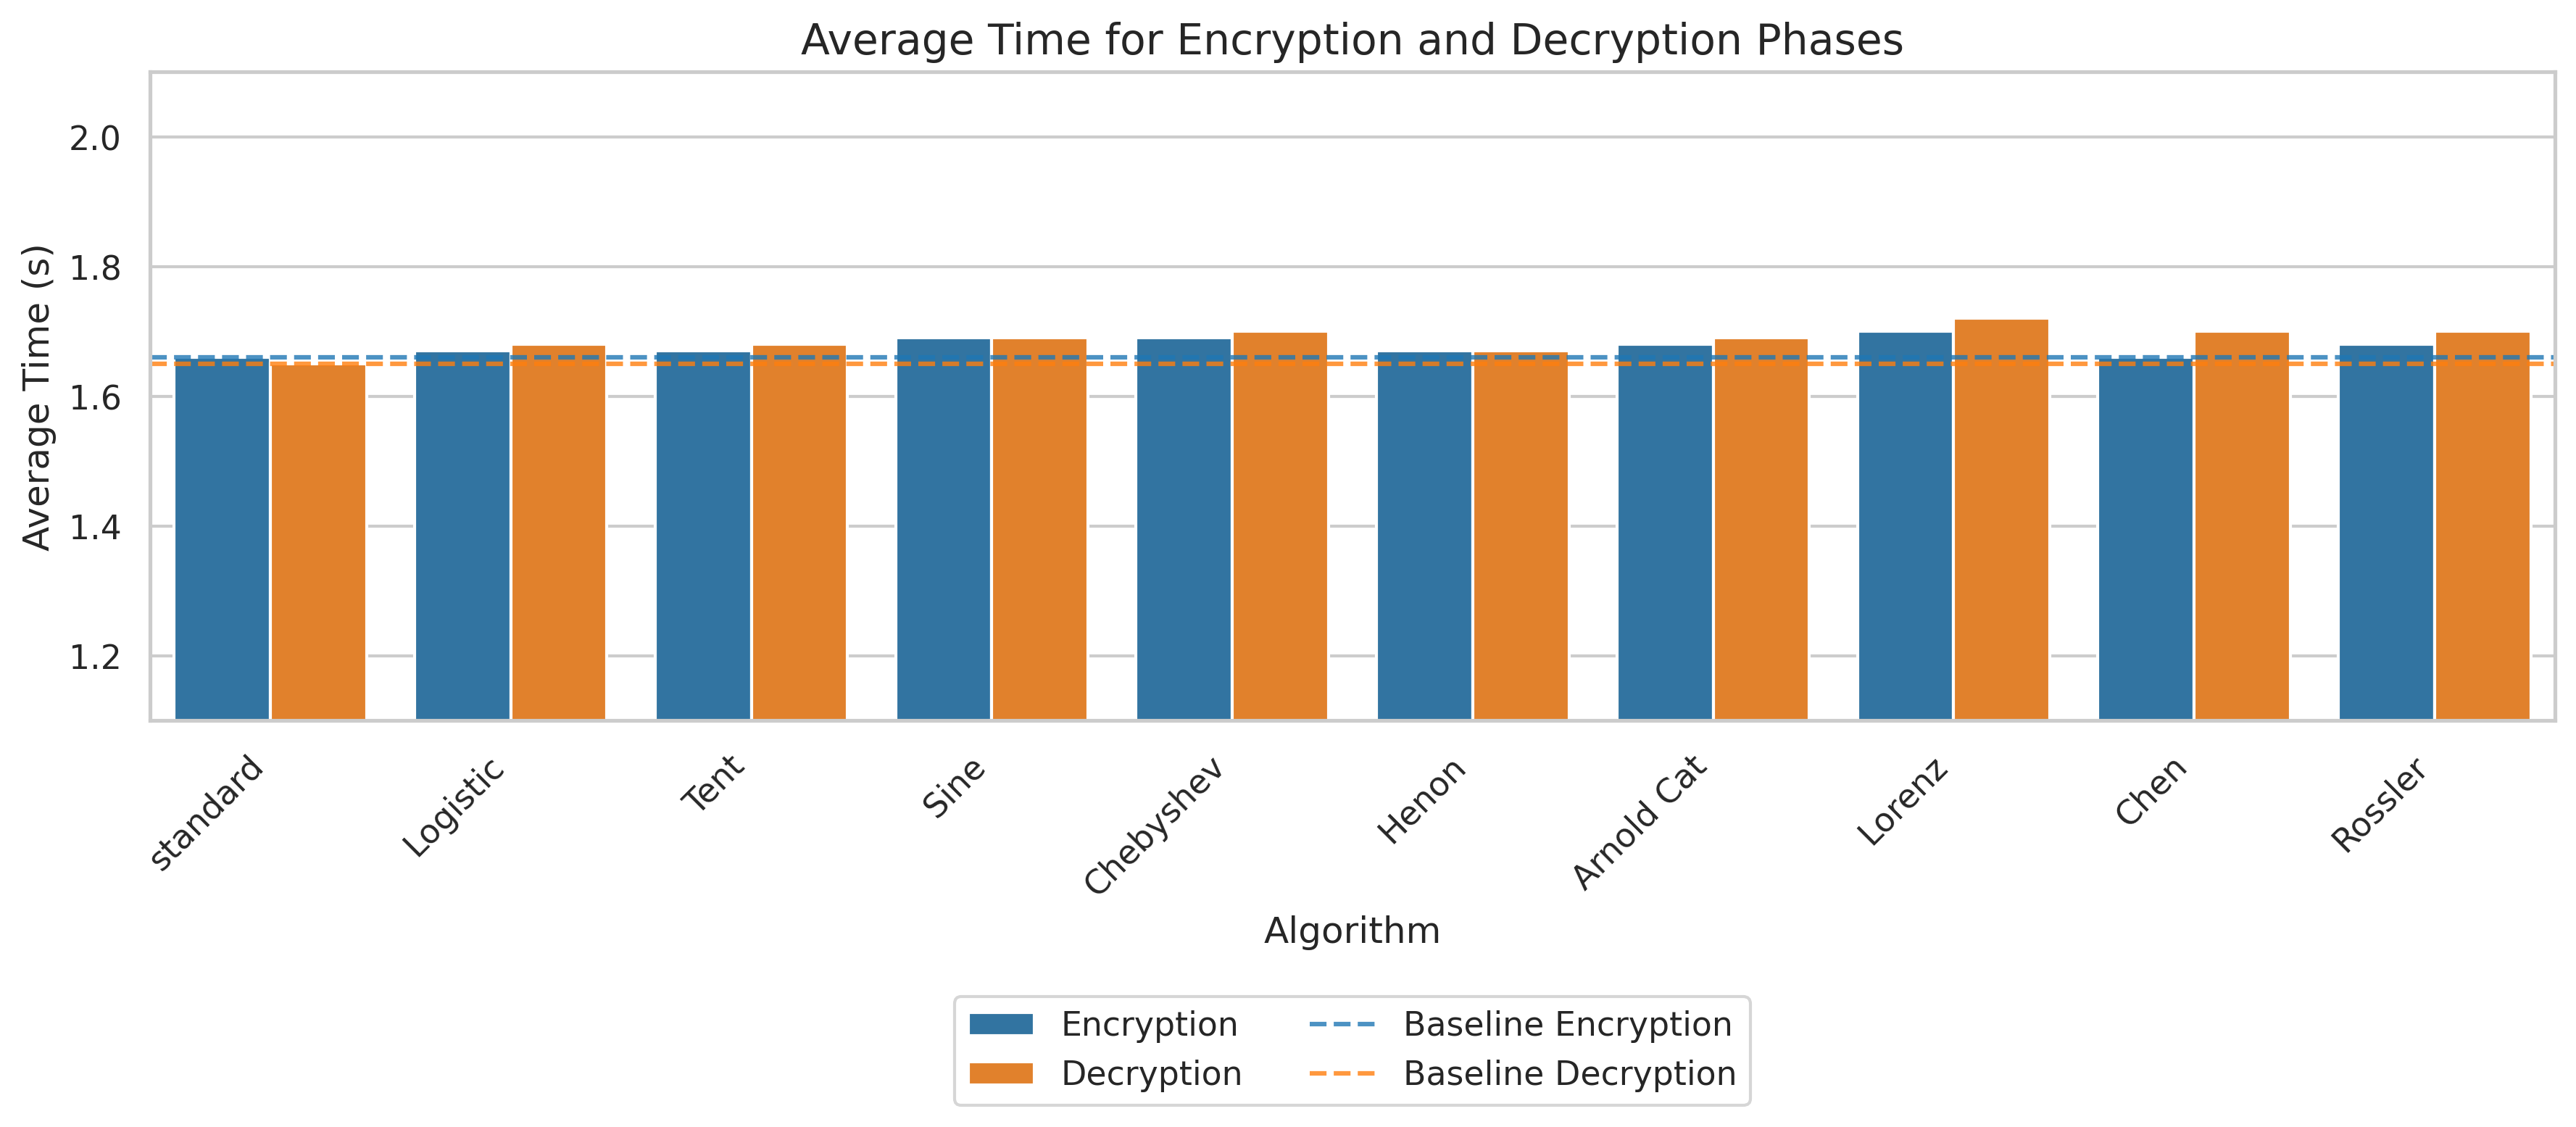
\includegraphics[width=0.9\textwidth]{images/Time_opb.png}
    \caption{Average execution time comparison for the \texttt{once-per-block} chaotic injection architecture against the standard AES baseline.}
    \label{fig:opb_time}
\end{figure}

\paragraph{Energy and Memory Optimization Strategy}
Applying the same constant-power proxy assumptions established in the previous section, the energetic savings yielded by this architectural adjustment are substantial. 
For instance, the Rössler map, which previously exhibited a simulated $\approx 24\%$ energy penalty, now limits the satellite's battery drain to a highly sustainable $\approx 3.2\%$ overhead. 

Crucially, this temporal and energetic optimization is achieved without imposing any supplementary memory footprint. 
In the embedded C codebase, transitioning between the two strategies requires exclusively repositioning the \textsc{updateChaos()} function call outside the block's main \texttt{for} loop, as illustrated in Listing~\ref{lst:chaosUpdate}.

\begin{clisting}[label={lst:chaosUpdate}]{Chaos update architectural repositioning}
static void Cipher(struct AES_CHAOS_ctx* ctx, state_t* state, const uint8_t* RoundKey) {
  // Strategy: Once-per-block chaos update
  updateChaos(ctx);

  uint8_t round = 0;
  AddRoundKey(0, state, RoundKey);

  for (round = 1; ; ++round)
  {
    // Strategy: Once-per-round chaos update
    // updateChaos(ctx);
    
    SubBytes(ctx, state);
    // ...
  }
  AddRoundKey(Nr, state, RoundKey);
}
\end{clisting}

Because this modification merely relocates the called function within the \textsc{Cipher()} frame, the maximum Stack size remains perfectly invariant. 
Consequently, the dynamic Heap allocation also mirrors the exact lightweight parameters analyzed in Figure~\ref{fig:memory_footprint}. 
This definitively proves that the \texttt{once-per-block} chaotic update strategy mathematically immunizes the cipher without violating the size, weight, or power (SWaP) constraints of SATCOM devices.

\paragraph{Transitioning to Empirical Side-Channel Cryptanalysis}
Having successfully parameterized the chaotic systems, validated their strict cryptographic randomness, and proven the high performance architectural viability of the \texttt{once-per-block} implementation, 
the foundational setup of this research is complete. 

The subsequent chapter will transition from defensive optimization to offensive cryptanalysis. 
A highly specialized Machine Learning model will be used to execute a catastrophic key recovery attack against the S-Box power leakage. 
This exact model will then be deployed against both the standard AES and the optimized chaotic variant, 
empirically demonstrating the real-world physical resilience provided by the chaotic scalar perturbation.


% ====================================================================================================

% ====================================================================================================


\chapter[ML-based side-channel attack simulation]{ML-based side-channel attack \\ simulation}

As the ultimate pragmatic validation of the proposed Machine Unlearning architecture, this chapter introduces a dedicated Machine Learning-based Side-Channel Attack (SCA) 
aiming for complete cryptographic key recovery. 

The threat model specifically targets the micro-architectural vulnerability introduced by the static Look-Up Table (LUT) execution of the AES-256-GCM S-Box. 
By detailing a custom Divide-and-Conquer cryptanalysis technique, this chapter first demonstrates the devastating effectiveness of the profiling attack against the standard deterministic cipher. 
Subsequently, the exact same offensive methodology is deployed against the chaotic-injected variant, empirically proving that the scalar perturbation is sufficient to completely neutralize the threat and immunize the simulated SATCOM infrastructure.

\section{Threat Model and Physical Leakage}
The architectural focus of the chaotic injection proposed by Kumar et al.~\cite{KumarPaper} is specifically tailored to counter side-channel threats targeting microcontrollers that rely on a Look-Up Table (LUT) to execute the AES \textsc{SubBytes} transformation. 
In these standard software implementations, every byte substitution requires the CPU to execute a deterministic read operation from the memory module holding the S-Box array.

The fundamental vulnerability of this architecture lies in the physical properties of the underlying hardware. 
In standard \texttt{Complementary Metal-Oxide-Semiconductor (CMOS)} technology, logic transitions, specifically charging capacitance of a data bus wire from a logic \texttt{0} to a logic \texttt{1}, require a measurable draw of electrical current. 
Consequently, as extensively formalized by Mangard et al. in their foundational side-channel analysis~\cite{HW_PROPOZIONALE_CONSUMO}, the power consumed during a memory transfer is directly proportional to the \textit{Hamming Weight (HW)} of the data word being moved. 
By observing the power trace of the LUT memory access, an attacker can directly infer the Hamming Weight of the substituted byte.

Conversely, modern high-end processors mitigate this vulnerability by utilizing dedicated cryptographic hardware extensions (such as AES-NI). 
These modules calculate the Galois Field $\mathrm{GF}(2^8)$ arithmetic dynamically in hardware logic gates within a few clock cycles, entirely bypassing the memory bus and nullifying the LUT leakage. 
However, integrating dedicated cryptographic silicon increases die area, design complexity, and manufacturing costs, especially for radiation-hardened space-grade processors.
While power constraints are generally not an issue for terrestrial Ground Stations, this overhead is strictly prohibitive for the space segment (satellites) and lightweight end-user devices. 
Constrained nodes such as handheld satellite phones, remote VSAT (Very Small Aperture Terminal) ground sensors, and IoT satellite transceivers simply cannot sustain the power requirements of dynamic hardware calculation, 
rendering the software LUT implementation a strictly necessary architectural compromise.

This rigid hardware constraint leaves the SATCOM infrastructure critically exposed to physical cryptanalysis. 
As briefly introduced in Chapter 2, an attacker can harvest this power leakage through multiple vectors. 
In modern \textit{Satellite-as-a-Service (SataaS)} architectures, inadequate logical isolation might allow malicious co-resident software to sample the shared hardware's power fluctuations. 
On a higher operational level, highly sophisticated adversaries could leverage supply-chain attacks to embed hardware trojans into the satellite's components prior to launch, establishing a covert physical monitoring channel. 
Most commonly, however, the most vulnerable attack surfaces are the remote, unattended end-user terminals (e.g., environmental IoT sensors or compromised satellite phones), which can be physically captured and probed with an oscilloscope to completely extract the network's cryptographic keys.

To rigorously simulate this threat model, this study adopts a standardized side-channel proof-of-concept methodology. 
Instead of relying on analog traces captured by a physical oscilloscope, this simulation utilizes the Hamming Weight of the S-Box output byte as a deterministic proxy for the power consumption. 
As validated by foundational Machine Learning cryptanalysis frameworks such as the ASCAD database by Prouff et al.~\cite{HW_proof-of-concept}, targeting the mathematically pure HW provides an ideal baseline to evaluate the absolute classification capabilities of the ML model.

\section{Attack Choices and Theoretical Comparison}
The cryptanalysis methodology proposed in this thesis emerges as a direct consequence of a critical analysis of the threat model exposed by Kumar et al.~\cite{KumarPaper}. 
In their foundational research, the authors employed machine learning techniques to analyze physical leakages, specifically the power consumption derived from the S-Box substitution, to perform a classification attack. 
Their primary objective was to analyze simulated, intercepted ciphertexts to infer high-level intelligence, such as classifying the specific type of message being transmitted (e.g., distinguishing between telemetry data and mission-critical payloads).

However, this thesis deliberately diverges from the methodology pursued in the reference paper due to a severe cryptographic limitation inherent in their simulated environment. 
In order to successfully perform a classification attack directly on ciphertexts, the ML model requires that identical plaintext blocks encrypted during different communication sessions produce the exact same ciphertext output, allowing the algorithm to recognize static structural patterns. 
This deterministic behavior is only achievable by utilizing deprecated and deeply insecure modes of operation, such as the Electronic Codebook (ECB). 

Deploying an ECB-like architecture is completely unrealistic for a critical and highly regulated environment such as SATCOM, 
effectively confining such an attack model to a purely theoretical exercise. 
Therefore, this study chooses to strictly adhere to current aerospace communication standards by employing the AES-256-GCM architecture. 
Operating within this robust, non-deterministic framework, this thesis simulates a significantly more devastating threat vector: complete cryptographic key recovery.

Ultimately, while the operational goals differ radically from the reference literature, successfully executing this advanced key recovery attack against the baseline AES-256-GCM will serve as the perfect benchmark. 
It will conclusively demonstrate that the proposed chaotic-injected implementation is capable of blinding the ML classifier, preventing it from exploiting physical leakages to extract any usable information.

\section{The Machine Learning-Assisted Attack}
The proposed cryptanalysis is a three-phase procedure that leverages the physical energy leakage of the S-Box to achieve a complete cryptographic key recovery. 
To render this theoretical micro-architectural vulnerability practically exploitable against the AES-256-GCM architecture, a Machine Learning classifier is employed as the core analytical engine.

\subsection{Profiling Phase and Data Collection}
Executing an ML-based Side-Channel Attack fundamentally requires a robust profiling phase, during which the classifier is trained on a substantial dataset to learn the hidden correlations between the physical leakages and the internal cryptographic states. 
In this threat model, aligning with standard profiling attack methodologies, the attacker is assumed to possess a ``clone device'' identical to the target satellite hardware. 
This allows the attacker to freely encrypt known data, monitor the hardware, and perfectly label the resulting leakages.

The profiling dataset generated for this study consists of 15000 distinct communication traces. 
As illustrated in Table~\ref{tab:training_data_sample}, each entry perfectly mirrors the information an attacker could intercept during a real SATCOM transmission: 
the public Initialization Vector (IV) and the corresponding sequence of physical leakages captured at the output of the S-Box substitution (represented by the Hamming Weight, HW). 
In a real-world physical attack, these discrete HW integers would simply be substituted by the analog voltage measurements extracted from an oscilloscope.

\begin{table}[htbp]
    \centering
    \footnotesize
    \setlength{\tabcolsep}{3.5pt}
    \resizebox{\textwidth}{!}{%
    \begin{tabular}{lcccccccccccc}
        \toprule
        \textbf{IV} & $\textbf{HW}_{\textbf{0}}$ & $\boldsymbol{\dots}$ & $\textbf{HW}_{\textbf{14}}$ & $\textbf{HW}_{\textbf{15}}$ & $\boldsymbol{\dots}$ & $\textbf{HW}_{\textbf{31}}$ & $\textbf{Target}_{\textbf{0}}$ & $\boldsymbol{\dots}$ & $\textbf{Target}_{\textbf{14}}$ & $\textbf{Target}_{\textbf{15}}$ & $\boldsymbol{\dots}$ & $\textbf{Target}_{\textbf{31}}$ \\
        \midrule
        {\scriptsize\texttt{8003709c39fc04246a7cea47}} & 5 & $\dots$ & 2 & 4 & $\dots$ & 4 & 188 & $\dots$ & 160 & 114 & $\dots$ & 226 \\
        {\scriptsize\texttt{7960e910e31d36bb3155aead}} & 2 & $\dots$ & 2 & 4 & $\dots$ & 4 &  12 & $\dots$ & 160 & 114 & $\dots$ & 139 \\
        {\scriptsize\texttt{62394bd9749faeb04fd48a1e}} & 4 & $\dots$ & 2 & 4 & $\dots$ & 7 & 184 & $\dots$ & 160 & 114 & $\dots$ & 127 \\
        $\vdots$ & $\vdots$ & $\ddots$ & $\vdots$ & $\vdots$ & $\ddots$ & $\vdots$ & $\vdots$ & $\ddots$ & $\vdots$ & $\vdots$ & $\ddots$ & $\vdots$ \\
        \bottomrule
    \end{tabular}%
    }
    \caption{Sample entries from the clone device's training dataset, displaying the public Initialization Vector (IV), sequential Hamming Weight features ($\text{HW}_0 \dots \text{HW}_{31}$), and the definitive target ciphertext byte values ($\text{Target}_0 \dots \text{Target}_{31}$).}
    \label{tab:training_data_sample}
\end{table}

To enable supervised learning, the profiling set also contains the definitive internal target values (\texttt{Target}) corresponding to each captured Hamming Weight. 
By mapping the intercepted IVs and HWs to these known targets, the ML algorithm can continually evaluate its classification accuracy, 
iteratively adjusting its internal decision pathways to minimize the error rate and build a highly accurate leakage profile.

Finally, during the active exploitation phase, the trained ML classifier is fed a structurally identical dataset harvested directly from the victim device. 
Crucially, this operational dataset is completely lacking of the internal target labels. 
Instead, the model must autonomously predict these unknown cryptographic variables by correlating the intercepted public IVs and the physical power leakages against its established profiling parameters.

\subsection{The Selected ML Architecture: Random Forest}
To execute the cryptanalysis phase, this study implements a \texttt{Random Forest} classifier~\cite{RandomForest}, deployed within the Python simulation environment via the \textsc{scikit-learn} library~\cite{scikit-learn}. 
As part of the ensemble learning family, the Random Forest algorithm is exceptionally suited for analyzing discrete, tabular datasets characterized by non-linear relationships, which perfectly describes the correlation between S-Box byte substitutions and hardware leakage. 

While Deep Neural Networks (DNNs) are heavily featured in modern side-channel literature, they were deliberately discarded for this specific threat model. 
Neural Networks require larger profiling datasets to converge accurately and demand significantly heavier computational resources. 
Given the restricted 15000-trace training set available in this simulation, a Random Forest guarantees superior classification accuracy with a fraction of the computational overhead, drastically outperforming a DNN under strict data availability constraints.

Architecturally, a Random Forest operates by constructing a multitude of independent binary decision trees during the training phase. 
When an input vector (the features) is fed into the system, each individual tree processes the data through a hierarchical sequence of logical conditions (nodes). 
Depending on whether the input satisfies these conditions, it traverses different branches until it reaches a terminal node (leaf), which represents that single tree's prediction.
The robustness of the Random Forest relies on three fundamental mechanisms:
\begin{itemize}
    \item \textbf{Bagging (Bootstrap Aggregating):} Instead of training every tree on the exact same dataset, each tree is fed a slightly different, randomly sampled subset of the original profiling data. 
    This forces individual trees to specialize in different mathematical patterns.

    \item \textbf{Feature Randomness:} Similarly, at every internal node split, the algorithm only considers a random subset of the available features (the HW values) rather than the entire array. 
    This structural variance ensures that the trees do not correlate with one another, preventing them from collectively anchoring onto a single dominant feature.

    \item \textbf{Ensemble Voting:} During the active attack phase, every tree in the forest independently outputs a prediction. 
    The final classification is determined by aggregating these individual decisions into a collective vote. 
    In the deployed Python simulation, the \textsc{predict()} function returns the absolute majority vote, 
    while the \textsc{predict\_proba()} method calculates the statistical probability distribution across all 256 possible byte values. 
    This probability vector is critical for the subsequent statistical aggregation.
\end{itemize}

To train the classifier, the model is fed a bidimensional matrix of \texttt{features} (the hardware leakages, structured with traces as rows and byte positions as columns), 
rigidly mapped against their corresponding \texttt{labels} (the known target internal states). 
The model is then compiled using the \textsc{fit} function, strictly adhering to the following hyperparameter configuration to maximize accuracy while preventing structural memorization:
\begin{itemize}
    \item \texttt{n\_estimators = 100}: The forest comprises exactly 100 independent decision trees, selected as the optimal equilibrium between computational speed and statistical accuracy.
    
    \item \texttt{max\_depth = 8}: The maximum hierarchical depth of any tree is capped at 8 layers. This structurally prevents the algorithm from endlessly branching to memorize the training data (\textit{overfitting}), forcing the model to learn generalized, robust physical leakage correlations.
    
    \item \texttt{min\_samples\_split = 20} and \texttt{min\_samples\_leaf = 10}: As secondary anti-overfitting mechanisms, an internal node requires at least 20 samples to authorize a further split, and any resulting terminal leaf must encompass a minimum of 10 samples. 
    This prevents the creation of hyperspecific, irrelevant branches driven by analog noise.

    \item \texttt{random\_state}: A fixed procedural seed is initialized to guarantee the absolute reproducibility of the simulated attack.
\end{itemize}

\begin{figure}[htbp]
    \centering
    \resizebox{\textwidth}{!}{%
    \begin{tikzpicture}[
        >=latex,
        node/.style={
            rectangle,
            rounded corners=3pt,
            draw=blue!50!black,
            line width=0.75pt,
            fill=blue!4,
            align=center,
            inner sep=6pt,
            minimum width=4.0cm,
            font=\scriptsize
        },
        leaf/.style={
            rectangle,
            rounded corners=3pt,
            draw=teal!60!black,
            line width=0.75pt,
            fill=teal!6,
            align=center,
            inner sep=4pt,
            text width=2.85cm,
            font=\scriptsize
        },
        branch/.style={
            fill=white,
            inner sep=2pt,
            font=\scriptsize\bfseries
        },
        edge/.style={
            draw=black!70,
            ->,
            line width=0.75pt
        }
    ]
        % --- ROOT NODE ---
        \node[node, fill=blue!8, line width=0.9pt] (root) at (0, 0) {
            \textbf{Root Node ($N = 5000$)}\\[2pt]
            $2000\;\mathtt{0x12} \;\mid\; 1500\;\mathtt{0x4A} \;\mid\; 1500\;\mathtt{0xFF}$\\[3pt]
            \textbf{Best Split:} $\text{HW}_0 \le 4.5$
        };

        % --- LEVEL 1 NODES ---
        \node[node] (left) at (-3.8, -2.5) {
            \textbf{Internal Node ($N = 2200$)}\\[2pt]
            $1900\;\mathtt{0x12} \;\mid\; 300\;\mathtt{0x4A} \;\mid\; 0\;\mathtt{0xFF}$\\[3pt]
            \textbf{Best Split:} $\text{HW}_0 \le 2.5$
        };

        \node[node] (right) at (3.8, -2.5) {
            \textbf{Internal Node ($N = 2800$)}\\[2pt]
            $100\;\mathtt{0x12} \;\mid\; 1200\;\mathtt{0x4A} \;\mid\; 1500\;\mathtt{0xFF}$\\[3pt]
            \textbf{Best Split:} $\text{HW}_0 \le 6.5$
        };

        % --- LEVEL 2 (LEAVES) ---
        \node[leaf] (leaf1) at (-5.7, -5.3) {
            \textbf{Leaf 1 ($N = 1800$)}\\[2pt]
            $1800\;\mathtt{0x12}$\\[2pt]
            \textit{\color{teal!60!black}($\mathtt{0x12}: 100\%$)}
        };

        \node[leaf] (leaf2) at (-1.9, -5.3) {
            \textbf{Leaf 2 ($N = 400$)}\\[2pt]
            $100\;\mathtt{0x12} \;\mid\; 300\;\mathtt{0x4A}$\\[2pt]
            \textit{\color{black!70}($\mathtt{0x12}: 25\%,\;\mathtt{0x4A}: 75\%$)}
        };

        \node[leaf] (leaf3) at (1.9, -5.3) {
            \textbf{Leaf 3 ($N = 1250$)}\\[2pt]
            $50\;\mathtt{0x12} \;\mid\; 1100\;\mathtt{0x4A}$\\
            $100\;\mathtt{0xFF}$\\[2pt]
            \textit{\color{black!70}($\mathtt{0x12}: 4\%,\;\mathtt{0x4A}: 88\%,$}\\
            \textit{\color{black!70}$\mathtt{0xFF}: 8\%$)}
        };

        \node[leaf] (leaf4) at (5.7, -5.3) {
            \textbf{Leaf 4 ($N = 1550$)}\\[2pt]
            $50\;\mathtt{0x12} \;\mid\; 100\;\mathtt{0x4A}$\\
            $1400\;\mathtt{0xFF}$\\[2pt]
            \textit{\color{teal!60!black}($\mathtt{0x12}: 3\%,\;\mathtt{0x4A}: 7\%,$}\\
            \textit{\color{teal!60!black}$\mathtt{0xFF}: 90\%$)}
        };

        % --- EDGES ---
        \draw[edge] (root) -- (left) node[branch, text=teal!60!black, pos=0.45, left=3pt] {True};
        \draw[edge] (root) -- (right) node[branch, text=red!65!black, pos=0.45, right=3pt] {False};

        \draw[edge] (left) -- (leaf1) node[branch, text=teal!60!black, pos=0.45, left=2pt] {True};
        \draw[edge] (left) -- (leaf2) node[branch, text=red!65!black, pos=0.45, right=2pt] {False};

        \draw[edge] (right) -- (leaf3) node[branch, text=teal!60!black, pos=0.45, left=2pt] {True};
        \draw[edge] (right) -- (leaf4) node[branch, text=red!65!black, pos=0.45, right=2pt] {False};

    \end{tikzpicture}%
    }
    \caption{Decision tree training (profiling) process over $N = 5000$ labeled traces. 
    At each internal node, the algorithm selects the Hamming Weight threshold ($\text{HW}_0 \le \tau$), partitioning the dataset into progressively purer leaf nodes.}
    \label{fig:rf_tree_training}
\end{figure}

\paragraph{Maximum Likelihood Estimation (MLE)}
In a real-world physical cryptanalysis scenario, relying on the classification of a single intercepted communication is highly prone to errors. 
The analog noise inherent in the hardware measurements could easily mask the true target value, causing the classifier to output an incorrect majority vote. 

To surgically bypass this physical limitation, the attack implements a Maximum Likelihood Estimation (MLE) algorithm. 
Instead of analyzing a single message, the attacker intercepts a batch of $N$ communications encrypted under the exact same unknown key. 
For every intercepted trace, the Random Forest utilizes the \textsc{predict\_proba()} function to generate a probability distribution array across all 256 possible byte candidates. 

The MLE algorithm then aggregates these discrete arrays, summing the logarithmic probabilities of each candidate across all $N$ traces. 
The candidate byte that accumulates the highest overall statistical probability is definitively selected as the correct key fraction. 
To ensure mathematical stability during the logarithmic summation, specifically to prevent undefined $\log(0)$ errors if the model assigns a flat $0\%$ probability to a candidate in a specific trace, 
an epsilon smoothing technique is applied, injecting a minimal $10^{-9}$ variation into the probability arrays.


\subsection{Attack Strategy and GCM Constraints}
The initial cryptanalysis strategy leveraged the dataset's variance to train the ML classifier to directly predict the byte values exiting the first S-Box substitution. 
Because this substitution occurs at the very beginning of the AES algorithm, the output of the $i$-th S-Box is defined as:

\begin{equation}
    S_{out}[i] = \textsc{SubBytes}(J_0[i] \oplus K_{P1}[i])
\end{equation}

where $J_0$ is the initial input block and $K_{P1}$ is the first half of the AES-256 master key. 
If the Random Forest successfully predicts $S_{out}[i]$, the attacker can exploit the public state of the algorithm to mathematically reverse the operation. 
Utilizing the \textsc{InvSubBytes}() function and the involutory property of the XOR operation ($A = B \oplus C \implies B = A \oplus C$), the secret key byte can be trivially recovered using the known public input block:

\begin{equation}
    K_{P1}[i] = J_0[i] \oplus \textsc{InvSubBytes}(S_{out}[i])
\end{equation}

However, two major structural challenges impede this straightforward key-recovery flow. 
First, AES-256 utilizes a 32-byte master key. This means the initial \textsc{AddRoundKey()} operation only consumes the first 16 bytes ($K_{P1} = K[0:15]$). 
The second half of the master key ($K_{P2} = K[16:31]$) is only injected during the subsequent first main round. 
While this could theoretically be addressed by extending the ML attack to predict the outputs of the second round's \textsc{SubBytes}() operation and algebraically rolling back the state, the second issue presents a strict mathematical roadblock.

Following SATCOM standards and the official NIST SP 800-38D specifications~\cite{GCM} for the GCM mode of operation, 
the preferred Initialization Vector (IV) length is exactly 12 bytes. 
To form the required 16-byte initial counter block ($J_0$) that enters the AES cipher, a fixed 32-bit counter is appended to the IV, 
resulting in the structural concatenation: $J_0 = \mathit{IV} \parallel \mathtt{0x00000002}$. 

While this deterministic padding is mathematically rigorous for standard encryption, it compromises the ML profiling phase. 
Because the last four input bytes are artificially forced to be constant ($\mathtt{0x00, 0x00, 0x00, 0x02}$) across every single communication, and the target key $K_{P1}$ remains fixed, the resulting S-Box outputs for byte indexes 12 through 15 never change (as previously observable in the static columns of Table~\ref{tab:training_data_sample}). 

Machine Learning classifiers inherently rely on data variance to establish correlations and recognize physical leakage patterns. 
The absolute staticity of these four bytes starves the Random Forest of any informational entropy, rendering it impossible to profile and predict the last four bytes of $K_{P1}$. 
Consequently, without recovering the complete 16-byte $K_{P1}$, computing the internal cipher state forwards to attack the second round ($K_{P2}$) is impossible, mandating the adoption of a more advanced algebraic Divide-and-Conquer strategy.

\paragraph{Phase 1: Recovery of the First 12 Key Bytes}
After training the Random Forest on the profiling dataset, the active attack phase is initiated by feeding the model a highly constrained operational dataset, 
typically containing only a hundred intercepted IVs and their corresponding physical power traces. 
Through the implementation of the Maximum Likelihood Estimation (MLE) algorithm, the model processes each intercepted communication to generate a 256-element probability vector for each of the first 12 bytes. 
Each index in this vector represents the statistical probability that the S-Box output corresponds to that specific byte value (e.g., $\mathbf{P}(S_{out}[i]) = [p_0, p_1, \dots, p_{255}]$).

For each of the first 12 bytes of $K_{P1}$, the candidate value with the highest aggregated probability is selected as the definitive prediction. 
This yields the following partially recovered state for the first S-Box output:
\begin{equation}
\text{Prediction\_S1}_{\text{out}} = \begin{bmatrix}
    P_0 & P_4 & P_8 & X_{12} \\
    P_1 & P_5 & P_9 & X_{13} \\
    P_2 & P_6 & P_{10} & X_{14} \\
    P_3 & P_7 & P_{11} & X_{15}
\end{bmatrix}
\end{equation}
where $P_i$ represents the $i$-th predicted byte, and $X_i$ denotes the four unpredictable bytes severely masked by the fixed $\mathtt{0x00000002}$ suffix.

Despite the missing column, the recovery of the first 12 key bytes remains entirely feasible. 
Because both the \textsc{SubBytes}() and \textsc{AddRoundKey()} operations process the state matrix strictly byte-by-byte, 
the spatial independence of the 16 bytes is rigorously preserved. 
Since the initial input block is completely known ($J_0 = \mathit{IV} \parallel \mathtt{0x00000002}$), the first section of the key is trivially retrieved through a direct algebraic derivation. 
Using the symbol $*$ to represent the unpredictable values, the extraction is mathematically formalized as follows (\textsc{InvSubBytes} $\equiv S^{-1}$):

\begin{equation}
\setlength{\arraycolsep}{3.5pt}
\begin{gathered}
    \text{Retrieved\_}K_{P1}[0:11] = J_0 \oplus \textsc{InvSubBytes}(\text{Prediction\_S1}_{\text{out}}) = \\[6pt]
    = \begin{bmatrix}
        J_0[0] & J_0[4] & J_0[8] & J_0[12] \\
        J_0[1] & J_0[5] & J_0[9] & J_0[13] \\
        J_0[2] & J_0[6] & J_0[10] & J_0[14] \\
        J_0[3] & J_0[7] & J_0[11] & J_0[15]
    \end{bmatrix}
    \oplus
    \textsc{InvSubBytes}
    \begin{bmatrix}
        P_0 & P_4 & P_8 & X_{12} \\
        P_1 & P_5 & P_9 & X_{13} \\
        P_2 & P_6 & P_{10} & X_{14} \\
        P_3 & P_7 & P_{11} & X_{15}
    \end{bmatrix} = \\[6pt]
    = \begin{bmatrix}
        J_0[0] \oplus S^{-1}(P_0) & J_0[4] \oplus S^{-1}(P_4) & J_0[8] \oplus S^{-1}(P_8) & * \\
        J_0[1] \oplus S^{-1}(P_1) & J_0[5] \oplus S^{-1}(P_5) & J_0[9] \oplus S^{-1}(P_9) & * \\
        J_0[2] \oplus S^{-1}(P_2) & J_0[6] \oplus S^{-1}(P_6) & J_0[10] \oplus S^{-1}(P_{10}) & * \\
        J_0[3] \oplus S^{-1}(P_3) & J_0[7] \oplus S^{-1}(P_7) & J_0[11] \oplus S^{-1}(P_{11}) & *
    \end{bmatrix}
    = \begin{bmatrix}
        K^R_0 & K^R_4 & K^R_8 & * \\
        K^R_1 & K^R_5 & K^R_9 & * \\
        K^R_2 & K^R_6 & K^R_{10} & * \\
        K^R_3 & K^R_7 & K^R_{11} & *
    \end{bmatrix}
\end{gathered}
\end{equation}

\newpage

\paragraph{Phase 2: Divide-and-Conquer Strategy}
Now that the first 12 bytes of $K_{P1}$ have been successfully retrieved, the cryptanalysis transitions to its second phase: 
recovering the remaining 20 bytes of the AES-256 state (comprising the 4 missing bytes of $K_{P1}$ and the entire 16-byte $K_{P2}$ round key).

However, the incomplete state of $K_{P1}$ presents a critical algebraic roadblock for the direct recovery of $K_{P2}$. 
This complication is structurally induced by the \textsc{ShiftRows()} and \textsc{MixColumns()} diffusion layers. 
During the first round, the \textsc{ShiftRows()} operation scatters the four unknown bytes from the state's last column, distributing exactly one unknown byte into each of the four columns. 
Subsequently, the \textsc{MixColumns()} routine processes these columns vertically, causing each single unknown byte of $K_{P1}$ to algebraically diffuse and ``infect'' an entire 4-byte column of the Round 1 output state ($State^{(1)}_{out}$).

Because the input to the second round is now heavily entangled with the unknown variables of $K_{P1}$, it becomes impossible to perfectly compute $State^{(1)}_{out}$. 
Consequently, even if a second Random Forest model perfectly predicts the S-Box outputs of the second round:
\begin{equation}
\text{Prediction\_S2}_{\text{out}} = \begin{bmatrix}
    Q_0 & Q_4 & Q_8 & Q_{12} \\
    Q_1 & Q_5 & Q_9 & Q_{13} \\
    Q_2 & Q_6 & Q_{10} & Q_{14} \\
    Q_3 & Q_7 & Q_{11} & Q_{15}
\end{bmatrix}
\end{equation}
the attacker can no longer use the simple matrix involution:
\begin{equation}
\text{Retrieved\_}K_{P2} = State^{(1)}_{out} \oplus \textsc{InvSubBytes}(\text{Prediction\_S2}_{\text{out}})
\end{equation}
to trivially retrieve the second half of the key, as $State^{(1)}_{out}$ is no longer a known public variable.

Nonetheless, the strict mathematical diffusion generated by the \textsc{ShiftRows()} and \textsc{MixColumns()} routines can be reverse-engineered to the attacker's advantage, 
strategically reducing the search space to make a localized brute-force attack highly feasible. 

This phase leverages the precise spatial permutation of the \textsc{ShiftRows()} operation. 
As established in the standard AES architecture, this function shifts the four unknown variables ($X_i$) of $K_{P1}$ diagonally, 
placing exactly one unknown variable into each of the four columns:
\[
\text{S1}_{\text{out}} = \begin{bmatrix}
    B_0 & B_4 & B_8 & X_{12} \\
    B_1 & B_5 & B_9 & X_{13} \\
    B_2 & B_6 & B_{10} & X_{14} \\
    B_3 & B_7 & B_{11} & X_{15}
\end{bmatrix}
\xrightarrow{\quad \textsc{ShiftRows} \quad}
Shift_{\text{out}} = \begin{bmatrix}
    B_0 & B_4 & B_8 & X_{12} \\
    B_5 & B_9 & X_{13} & B_1 \\
    B_{10} & X_{14} & B_2 & B_6 \\
    X_{15} & B_3 & B_7 & B_{11}
\end{bmatrix}
\]
This spatial distribution synergizes perfectly with the subsequent \textsc{MixColumns()} routine. 
Because \textsc{MixColumns()} operates strictly on a column-by-column basis in $\mathrm{GF}(2^8)$, 
where each output byte is algebraically influenced only by the four input bytes of its own column, the diffusion of the unknowns is rigidly isolated. 
After \textsc{MixColumns()}, each column of the state depends exclusively on a \textit{single} unknown variable: $X_{15}$ for Column 0, $X_{14}$ for Column 1, $X_{13}$ for Column 2, and $X_{12}$ for Column 3. 

Thanks to the byte-by-byte nature of the subsequent \textsc{AddRoundKey()} and \textsc{SubBytes()} operations, 
this separation allows the attacker to execute a Divide-and-Conquer strategy. 
Instead of attacking the state as a whole, the attacker can iteratively evaluate all 256 possible values for a single unknown variable per column, generating isolated partial key guesses.

For instance, to generate the hypothesis set for the first column (Column 0), the attack iterates a hypothetical guess $i \in [0, 255]$ for the unknown variable $X_{15}$. 
This guess is combined with the three known public bytes ($B_0, B_5, B_{10}$) and processed through the \textsc{MixColumns()} matrix multiplication:
\[
Shift_{\text{out}}[0] = \begin{bmatrix}
    B_0 \\
    B_5 \\
    B_{10} \\
    i
\end{bmatrix}
\xrightarrow{\quad \textsc{MixColumns} \quad}
Mix_{\text{out}}[0] = \begin{bmatrix}
    M_0 \\
    M_1 \\
    M_2 \\
    M_3
\end{bmatrix}
\]

Simultaneously, the first column of the second Random Forest prediction ($\text{Prediction\_S2}_{\text{out}}$) 
is passed backwards through the \textsc{InvSubBytes()} function to obtain the theoretical output of the second \textsc{AddRoundKey()} layer:
\begin{equation}
    \textsc{AddRoundKey}_{\text{out}}[0] = S^{-1}\!\left(\text{Prediction\_S2}_{\text{out}}[0]\right)
    = \begin{bmatrix}
        S^{-1}(Q_0) \\
        S^{-1}(Q_1) \\
        S^{-1}(Q_2) \\
        S^{-1}(Q_3)
    \end{bmatrix}
    = \begin{bmatrix}
        A_0 \\
        A_1 \\
        A_2 \\
        A_3
    \end{bmatrix}
\end{equation}

By exploiting the involutory XOR property, a partial key prediction for $K_{P2}$, dependent on the specific guess $i$, is mathematically derived:
\begin{equation}
    K_{P2}[0:3]^{i} = \textsc{AddRoundKey}_{\text{out}}[0] \oplus Mix_{\text{out}}[0] 
    = \begin{bmatrix}
        K^{i}_{16} \\
        K^{i}_{17} \\
        K^{i}_{18} \\
        K^{i}_{19}
    \end{bmatrix}
\end{equation}
This partial $K_{P2}$ vector is cached and mapped to its corresponding guess $i$. 
This process is repeated 256 times for Column 0, and subsequently repeated for the remaining three columns, resulting in four independent sets of 256 partial hypotheses.

\paragraph{Final Phase: Reduced Brute-Force and HW Optimization}
Ultimately, the Divide-and-Conquer phase yields a structured combinatorial space. 
The final attack stage consists of aggregating one hypothesis from each of the four column sets to construct a full 32-byte candidate key:
\[
Key_{\text{candidate}} = K_{P1}[0:11] \parallel (X_{12}^h, X_{13}^l, X_{14}^j, X_{15}^i) \parallel (K_{P2}^{h}, K_{P2}^{l}, K_{P2}^{j}, K_{P2}^{i})
\]
Leveraging the Galois/Counter Mode (GCM), the attack validates the correct candidate by utilizing it to decrypt an eavesdropped ciphertext. 
If the locally computed GMAC tag matches the intercepted authentication tag, the key is confirmed as mathematically correct.

Through this methodology, the theoretical AES-256 search space is catastrophically reduced from an impossible $2^{256}$ down to $256^4 = 2^{32}$, 
rendering the brute-force phase computationally trivial. 

Furthermore, a significant micro-architectural optimization can be deployed to drastically reduce this space even further. 
While the static nature of the $J_0$ padding prevents the Random Forest from predicting the exact byte values of $X_{12}\dots X_{15}$, 
a physical side-channel trace still perfectly leaks the \textit{Hamming Weight} (HW) of those constant bytes. 
By knowing exactly how many active bits ('1's) are present in the target byte, the attacker can preemptively filter the 256 iterations. 

For instance, if the intercepted analog leakage indicates $\text{HW} = 1$, combinatorial mathematics dictates that only $\binom{8}{1} = 8$ bytes possess this property. 
Even in the statistical worst-case scenario where the leakage indicates $\text{HW} = 4$, the number of viable candidates drops to exactly:
\[
    \binom{8}{4} = \frac{8!}{4!(8-4)!} = 70 \text{ candidates.}
\]
By dynamically filtering the Divide-and-Conquer loops based on the physical HW leakage, the maximum theoretical search space plummets from $2^{32}$ down to an absolute worst-case of $70^4 = 24010000$ iterations. 
This final optimization guarantees a complete AES-256 key recovery in mere seconds on any standard personal computer, completely breaking the cipher's confidentiality.

\section{Empirical Attack Results}
\paragraph{Baseline Vulnerability: Standard AES-256-GCM}
To establish a baseline, the ML-assisted cryptanalysis was first executed against the standard, unprotected AES-256-GCM implementation utilizing the known target key: \\
\texttt{0f1080c9231bfcd6209f100ea59cf6722581ed9cca2d3dd7a3453c1e7f84ed8e}.

The Random Forest model seamlessly recovered the first 12 bytes of $K_{P1}$ with extreme precision. 
As illustrated in Figure~\ref{fig:std_attack}, the MLE algorithm perfectly isolated the correct byte value from the 256 candidates. 
The statistical confidence of the model is evident in the logarithmic score disparity: 
the correct value accumulated a score exceeding 1500, while all incorrect candidates remained suppressed below 500. 

\begin{figure}[H]
    \centering
    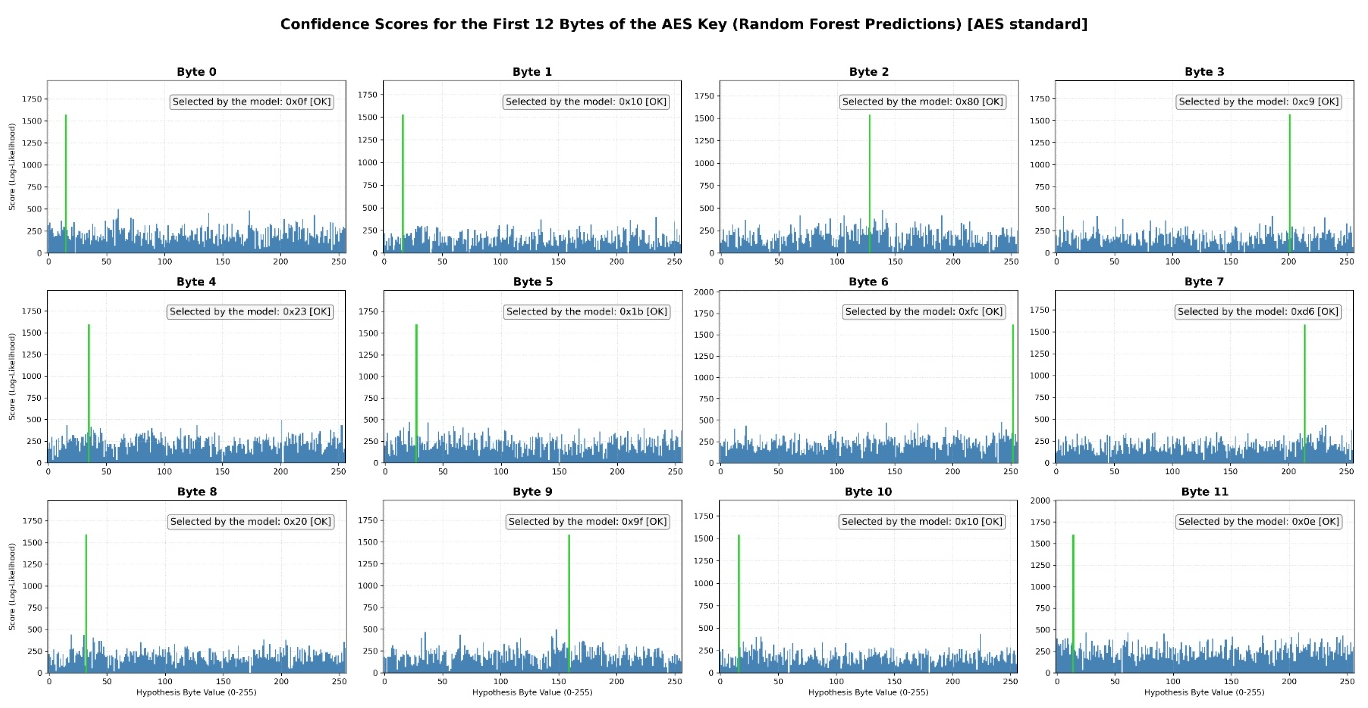
\includegraphics[width=0.75\textwidth]{images/standard_attack_res.png}
    \caption{MLE probability scores for the Random Forest prediction of the first 12 key bytes on the standard AES-256-GCM architecture. The green bar represents the confidence score achieved by the model for the predicted byte value.}
    \label{fig:std_attack}
\end{figure}

Following the successful Phase 1 extraction, the Divide-and-Conquer algorithm successfully profiled the Hamming Weights of the missing variables, 
generating the hypotheses files. The brute-force phase immediately followed, confirming a complete and catastrophic key recovery in less than half of the worst-case search space.

\begin{lightterminal}
--- Phase 1: First 12 Bytes Extraction ---
Byte 0 under analysis...  -> Found: 0f
[...]
Byte 11 under analysis... -> Found: 0e
[*] Found K1 portion: 0f1080c9231bfcd6209f100e (MATCH)

--- Phase 2: Divide-and-Conquer & Brute Force ---
[*] Generating hypotheses for columns 0-3 based on HW leakage...
[*] Hypotheses saved. Starting brute-force search...
[!!!] MASTER KEY FOUND [!!!]
Key: 0f1080c9231bfcd6209f100ea59cf6722581ed9cca2d3dd7a3453c1e7f84ed8e
Progress: 544096 / 1229312 keys tested
\end{lightterminal}

\paragraph{Chaotic Resilience: Once-per-Block Implementation}
Conversely, the exact same attack methodology, utilizing the identical key, IV set, and profiling parameters, 
was deployed against the AES variant protected by the \texttt{once-per-block} Logistic Map injection.

The Phase 1 extraction failed entirely. As shown in Figure~\ref{fig:lgt_attack}, 
the chaotic perturbation effectively masked the physical leakage, severely flattening the MLE probability distributions. 
The model managed to correctly identify only two bytes out of twelve. Given the flattened score distributions ($\approx 400$ for all candidates), these two matches represent mere statistical variance (a $1/256$ baseline probability) rather than genuine model convergence. 

\begin{figure}[htbp]
    \centering
    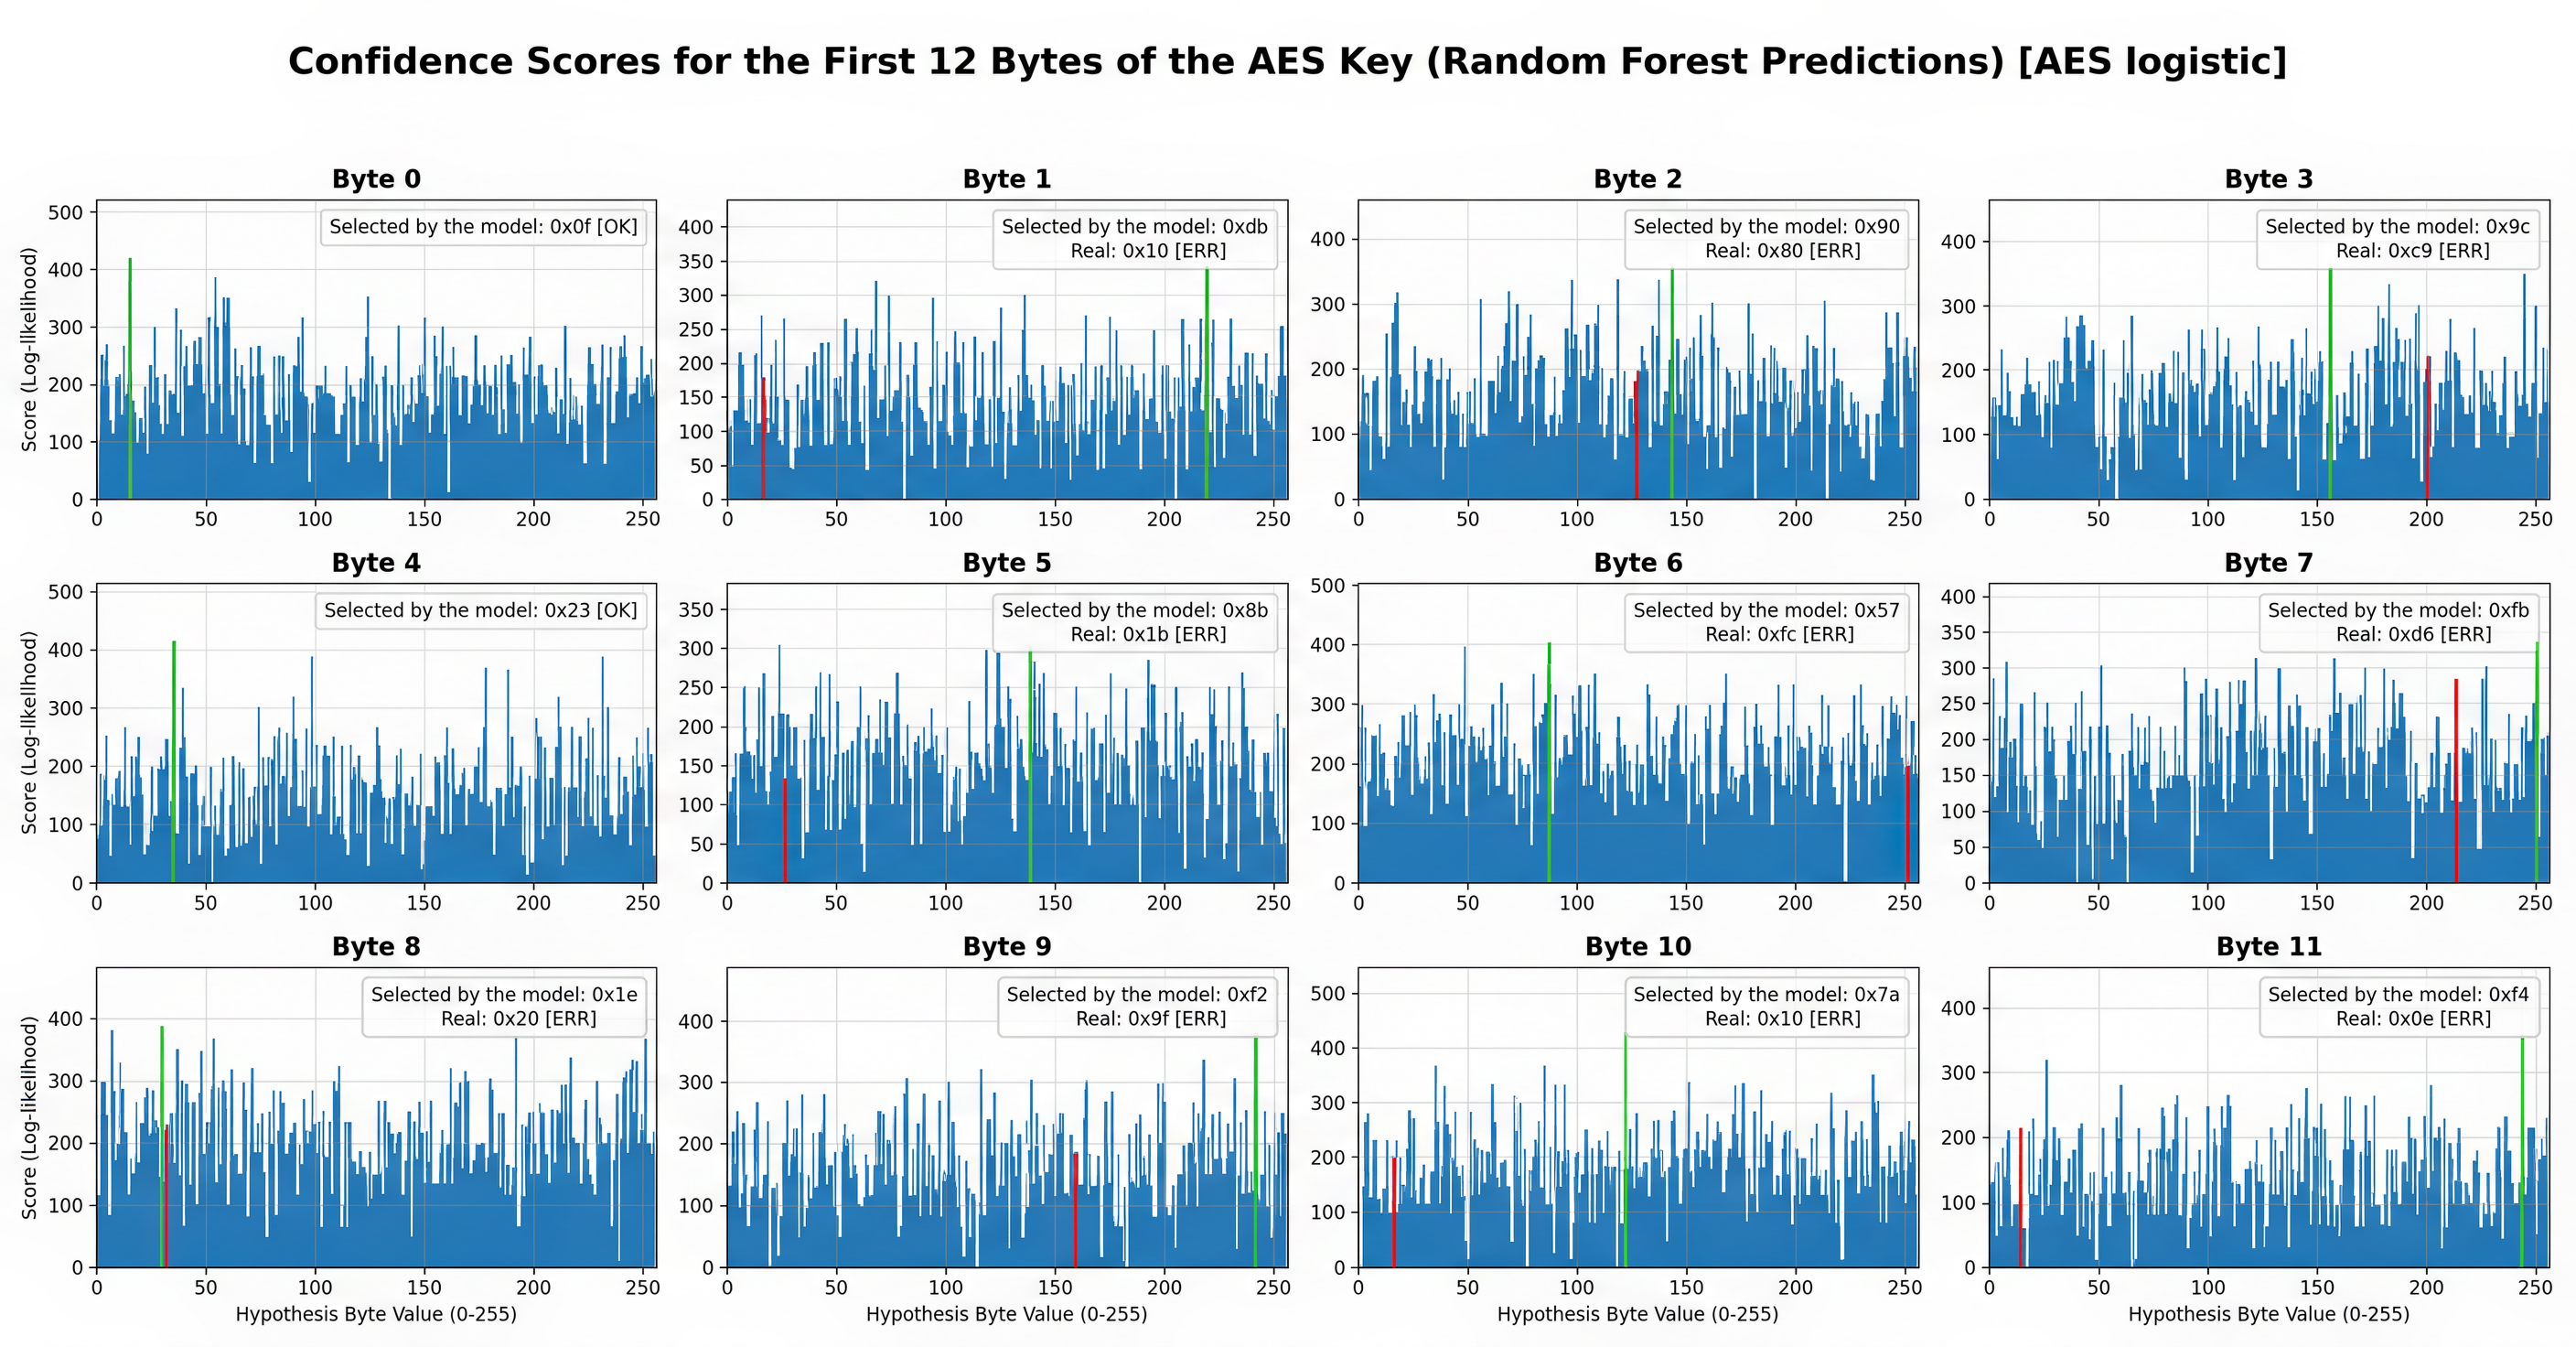
\includegraphics[width=0.75\textwidth]{images/logistic_attack_res.png}
    \caption{Flattened MLE probability scores on chaotic-injected AES using the \texttt{once-per-block} Logistic Map. As in Figure~\ref{fig:std_attack}, the green bar shows the predicted value's confidence score, while the red bar highlights the actual key byte's score upon misprediction.}
    \label{fig:lgt_attack}
\end{figure}

Because the Divide-and-Conquer algorithm strictly requires the absolute certainty of all first 12 bytes of $K_{P1}$ to correctly simulate the \textsc{MixColumns} algebraic diffusion, 
providing it with an incorrect $K_{P1}$ fragment mathematically breaks the hypothesis generation. 
Consequently, the ensuing brute-force search iterates over an entirely flawed state, resulting in a definitive failure to recover the key.

\begin{lightterminal}
--- Phase 1: First 12 Bytes Extraction ---
Byte 0 under analysis...  -> Found: 0f
Byte 1 under analysis...  -> Found: db (WRONG)
[...]
Byte 11 under analysis... -> Found: f4 (WRONG)
[*] Found K1 portion: 0fdb909c238b57fb1ef27af4
--- Phase 2: Divide-and-Conquer & Brute Force ---
[*] Generating hypotheses for columns 0-3 based on HW leakage...
[*] Hypotheses saved. Starting brute-force search...
No key found after testing 19208000 keys.
\end{lightterminal}

\paragraph{Average Success Rate across Chaotic Maps}
To formalize the ML classification resilience across the different dynamical systems, an automated iterative benchmark consisting of 1,000 independent attack executions was conducted for each map. 
This extensive sampling nullifies the impact of isolated, statistically lucky guesses, yielding the true average prediction accuracy for the initial 12 bytes.

\begin{table}[htbp]
    \centering
    \begin{tabular}{lc}
        \toprule
        \textbf{Chaotic Map} & \textbf{Average Success Rate (\%)} \\
        \midrule
        Standard (Unprotected) & 100.00 \\
        \midrule
        Logistic               &   0.91 \\
        Tent                   &   0.32 \\
        Sine                   &   0.30 \\
        Chebyshev              &   0.31 \\
        H\'enon                  &  25.14 \\
        Arnold                 &   0.28 \\
        Lorenz                 &  17.32 \\
        Chen                   &   0.00 \\
        R\"ossler                &   0.24 \\
        \bottomrule
    \end{tabular}
    \caption{Average key recovery success rate (\%) across the baseline (unprotected) implementation and the evaluated chaotic maps.}
    \label{tab:success_rates}
\end{table}

The empirical data reported in Table~\ref{tab:success_rates} demonstrates that the chaotic injection effectively neutralizes the profiling attack. 
Maps such as Chen completely sever the correlation, yielding a $0.00\%$ success rate. 

While the discrete H\'enon map exhibited the highest relative vulnerability with a $25.14\%$ success rate, this figure is highly misleading from a cryptographic perspective. 
A $25\%$ accuracy on a 12-byte target equates to correctly predicting only 3 bytes on average. This leaves 9 bytes completely unknown in $K_{P1}$ alone, introducing an immediate internal search space of $256^9 \approx 4.7 \times 10^{21}$ combinations before the Phase 2 algorithm can even begin. 
Therefore, even the weakest evaluated chaotic map successfully renders the side-channel key recovery computationally impossible, proving the absolute defensive viability of the \texttt{once-per-block} architecture.


\chapter{Conclusions}
As demonstrated through the empirical and analytical evaluations conducted in this thesis, 
the chaotic S-Box injection mechanism proposed by Kumar et al.~\cite{KumarPaper} provides robust software-level resilience against Machine Learning-assisted Side-Channel Attacks targeting the AES \textsc{SubBytes} routine. 
Crucially, this study proves that such cryptographic immunity is fully preserved even when collapsing the full chaotic state matrix into a single scalar perturbation weight, effectively neutralizing attacks that rely on the deterministic physical leakage of standard Look-Up Tables (LUTs).

The computational benchmarks performed under the baseline \texttt{once-per-round} update strategy highlighted a clear trade-off between mathematical complexity and performance. 
Lightweight one-dimensional discrete maps (such as Logistic and Tent) and two-dimensional maps (H\'enon and Arnold Cat) achieved strong side-channel resistance while maintaining a moderate time, throughput, and energy overhead, making them viable for resource-constrained environments. 
Conversely, trigonometric maps and three-dimensional continuous ODE systems (Lorenz, Chen, R\"ossler) imposed excessive computational penalties (exceeding $+20\%$ overhead), rendering them unsuitable for strict aerospace SWaP (Size, Weight, and Power) budgets under this update frequency.

To resolve this bottleneck, this thesis introduced and validated the \texttt{once-per-block} update optimization. 
The empirical results proved that updating the chaotic state once per 128-bit block flattens the temporal and energetic overhead across all evaluated systems, bringing lightweight maps down to a negligible $\approx 0.5\% - 1.5\%$ penalty and complex 3D systems below $4\%$,
while keeping the memory footprint completely invariant (at most 56 extra bytes).
Most importantly, the offensive cryptanalysis confirmed that this architectural optimization does not compromise security: 
while the Random Forest and Divide-and-Conquer attack achieved a $100\%$ key recovery rate on standard AES-256-GCM, it failed catastrophically against the \texttt{once-per-block} chaotic variants, 
rendering complete key extraction computationally infeasible.

Finally, due to its purely software-defined nature, this chaotic AES-256-GCM architecture offers a major operational advantage for the SATCOM domain. 
It can be deployed via Over-the-Air (OTA) firmware updates onto legacy spacecraft and existing embedded end-user terminals without requiring any physical hardware modifications, 
providing an immediate, cost-effective defense layer against modern side-channel threats.

\section{Future Work}
While this study establishes a solid proof-of-concept for lightweight chaotic masking in SATCOM, several research avenues remain open to transition this architecture toward flight-ready deployment:

\begin{itemize}
    \item \textbf{Physical Hardware and Oscilloscope Validation:} Moving beyond simulated Hamming Weight (HW) leakage models, future work should deploy the C codebase onto physical embedded targets to capture real analog power consumption and Electromagnetic traces via an oscilloscope. 
    This would validate the cipher's resilience against real-world signal-to-noise ratios and hardware-specific leakage effects.

    \item \textbf{Rad-Hard FPGA and Assembly Optimization:} Implementing the proposed chaotic cipher on radiation-hardened (rad-hard) FPGAs typically utilized in space segments would enable precise, 
    hardware-level timing and Joule dissipation measurements. In parallel, rewriting the core chaotic routines using a hybrid C-Assembly approach, inspired by the OpenSSL cryptographic library, could push software execution efficiency even closer to native hardware speeds.

    \item \textbf{Fixed-Point Arithmetic Migration:} To eliminate reliance on Floating-Point Units (FPUs) on low-power microcontrollers, and as a prerequisite for efficient FPGA synthesis, 
    future iterations should translate the chaotic map equations from floating-point (\texttt{double}) to fixed-point integer arithmetic. 
    This would guarantee cross-platform bit-level determinism and reduce energy consumption, while requiring careful analysis to mitigate \textit{dynamical degradation} and preserve cryptographic entropy.
    
    \item \textbf{Deep Learning-Based Cryptanalysis:} Finally, the \texttt{once-per-block} architecture should be stress-tested against more aggressive profiling adversaries utilizing Deep Learning models (such as Convolutional Neural Networks or Multi-Layer Perceptrons) trained on substantially larger datasets ($>100,000$ traces).
\end{itemize}


% New page for the bibliography
\newpage
\printbibliography[heading=bibintoc, title={Bibliography}]

\cleardoublepage
\chapter*{Ringraziamenti}
\thispagestyle{empty}

Per iniziare, ringrazio chi ha reso possibile il conseguimento di questo percorso senza mai pretendere nulla in cambio:
i miei genitori, che in ogni momento mi hanno sempre supportato nel corso della mia crescita fino ad arrivare qui.

Ringrazio anche mio fratello e mia sorella, i quali con la loro presenza hanno contribuito a rendermi la persona che sono oggi.

Doveroso è anche il ringraziamento al professor Casalicchio per avermi seguito con costanza e disponibilità
durante il periodo di tirocinio e nella stesura di questa tesi.

In ultimo, ringrazio il miglior gruppo di amici che potessi mai desiderare di trovare, che mi hanno accompagnato in questi anni di studio
non solo rendendoli estremamente più leggeri, ma probabilmente anche i tre migliori anni della mia vita, colmando le mie
giornate di divertimento e spenzieratezza.

Tra questi, un grazie speciale va a colei che da due anni è quotidianamente al mio fianco.


\end{document}